\section{Measurement Techniques}
Visible light has frequencies in the THz range which is well beyond the capabilites of modern electronics to directly measure so a number of clever strategies have been developed to measure the spectral quality of laser systems.
The performance of \gls*{ps} and \gls{pdh} frequency stabilisation has been characterised using a number of methods which are detailed here.
Spectral linewidth is the principle metric by which stabilisation techniques are compared and it can be considered over a range of timescales with different implications.
Short timescales measurements, less than a second, indicate the narrowness of the frequency spectrum and are useful when considering frequency dependent interactions, such as those with atoms or optical cavities.
Long timescale measurements, minutes to hours, are useful to determine the stability of the laser and its succeptability to frequency drift and the robustness of the locking scheme.

\subsection{Heterodyne Methods}

Heterodyning is a technique, invented by Canadian Reginald Feessenden in 1901, which mixes two frequencies to produce a new frequency~\cite{cooper_physics_2001}.
The technique can be used to examine the spectral properties of lasers as the newly produced frequencies can be tailored such that they are easily measurable by photodetectors and spectrum analysers.

Laser frequency spectrum measurements using heterodyne technique are simple to implement with the correct equipment.
The two laser beams are combined such that they copropagate, requiring some mirrors and a beamsplitter/combiner, and then focussed onto a high-bandwidth photodetector, where the bandwidth is dependent on the desired resolution.
The signal from the detector can then be fed into an equally high bandwidth spectrum analyser which will display the frequency spectrum of the intensity of the light on the detector.

\subsubsection{Basic Theory}
In the electrical signals context heterodyning involves the `mixing' or multiplying of two signals (e.g. two sine waves) to produce two different signals with frequencies equal to the difference and sum of the original frequencies:
\begin{equation}
\sin(\theta_1)\sin(\theta_2) = \frac{1}{2} \cos(\theta_1-\theta_2) - \frac{1}{2} \cos(\theta_1+\theta_2).
\end{equation}

In the optical context this is achieved due to the interference term accrued when squaring the electric field in order to calculate the intensity detected by the photodetector. The intensity of an electric field is given by:
\begin{equation}
I(t) = \frac{c\epsilon_0}{2}|E|^2.
\end{equation}

For two copropagating lasers with electric fields $E_{1, 2}$ and angular frequencies $\omega_{1, 2}$ we can write
\begin{equation}
E_{i}(t) = \sin(\omega_{i}t).
\end{equation}
The electric field at the detector, $E_T$, is given by the sum of $E_{1}$ and $E_{2}$, and thus the intensity is given by,
\begin{align}
I(t) &= |E_1(t) + E_2(t)|^2\nonumber\\
&= |E_1(t)|^2 + E_1(t)E_2^*(t) + |E_2(t)|^2.
\end{align}
The interference term, $E_1(t)E_2(t)$, allows for the spectral measurements with optical signals as
\begin{align}
E_1(t)E_2(t) &= \sin(\omega_1 t) \sin(\omega_2 t) \notag \\
&= \frac{1}{2} (\cos([\omega_1-\omega_2]t) - \cos([\omega_1+\omega_2]t)), \label{equation:hetero}
\end{align}
and if $\omega_{1,2}$ are appropriately selected then the first term in Equation~\ref{equation:hetero} is measurable.
The difference in frequency ideally should be fairly small, less than a few GHz, which can often be induced on lasers with the same frequency by \glspl{aom} or \glspl{eom}.

The equations presented above provide an obviously na\"ive approach as the frequency spread of the lasers is non-zero but gives a sufficient demonstration of the basis of the heterodyne method.
The spectral profile of the heterodyne signal is formed by the convolution of the spectral profiles of the component lasers, thus strategies are required in order to resolve the lineshape of a single laser.



\subsubsection{Frequency Reference}
One method of resolving the lineshape of a single laser is to use a second laser known to have a frequency lineshape much narrower than the laser of interest so that the convolved lineshape is the same as the lineshape of the laser of interest.
This method has some limitations in its application as it is only useful for resolving the lineshape of lasers with relatively wide specral width.
This method is shown in Figure~\ref{figure:heterodyne_reference}.

\begin{figure}
    %\centering
    \begin{subfigure}{0.49\linewidth}
    %\centering
    \includegraphics{part1/Figs/HeterodyneReferenceLaser.pdf}
    \end{subfigure}
    \begin{subfigure}{0.49\linewidth}
    %\centering
    %% Creator: Matplotlib, PGF backend
%%
%% To include the figure in your LaTeX document, write
%%   \input{<filename>.pgf}
%%
%% Make sure the required packages are loaded in your preamble
%%   \usepackage{pgf}
%%
%% Figures using additional raster images can only be included by \input if
%% they are in the same directory as the main LaTeX file. For loading figures
%% from other directories you can use the `import` package
%%   \usepackage{import}
%% and then include the figures with
%%   \import{<path to file>}{<filename>.pgf}
%%
%% Matplotlib used the following preamble
%%
\begingroup%
\makeatletter%
\begin{pgfpicture}%
\pgfpathrectangle{\pgfpointorigin}{\pgfqpoint{2.855000in}{1.427500in}}%
\pgfusepath{use as bounding box, clip}%
\begin{pgfscope}%
\pgfsetbuttcap%
\pgfsetmiterjoin%
\definecolor{currentfill}{rgb}{1.000000,1.000000,1.000000}%
\pgfsetfillcolor{currentfill}%
\pgfsetlinewidth{0.000000pt}%
\definecolor{currentstroke}{rgb}{1.000000,1.000000,1.000000}%
\pgfsetstrokecolor{currentstroke}%
\pgfsetdash{}{0pt}%
\pgfpathmoveto{\pgfqpoint{0.000000in}{0.000000in}}%
\pgfpathlineto{\pgfqpoint{2.855000in}{0.000000in}}%
\pgfpathlineto{\pgfqpoint{2.855000in}{1.427500in}}%
\pgfpathlineto{\pgfqpoint{0.000000in}{1.427500in}}%
\pgfpathclose%
\pgfusepath{fill}%
\end{pgfscope}%
\begin{pgfscope}%
\pgfsetbuttcap%
\pgfsetmiterjoin%
\definecolor{currentfill}{rgb}{1.000000,1.000000,1.000000}%
\pgfsetfillcolor{currentfill}%
\pgfsetlinewidth{0.000000pt}%
\definecolor{currentstroke}{rgb}{0.000000,0.000000,0.000000}%
\pgfsetstrokecolor{currentstroke}%
\pgfsetstrokeopacity{0.000000}%
\pgfsetdash{}{0pt}%
\pgfpathmoveto{\pgfqpoint{0.342732in}{0.521851in}}%
\pgfpathlineto{\pgfqpoint{1.130154in}{0.521851in}}%
\pgfpathlineto{\pgfqpoint{1.130154in}{1.277500in}}%
\pgfpathlineto{\pgfqpoint{0.342732in}{1.277500in}}%
\pgfpathclose%
\pgfusepath{fill}%
\end{pgfscope}%
\begin{pgfscope}%
\pgfpathrectangle{\pgfqpoint{0.342732in}{0.521851in}}{\pgfqpoint{0.787423in}{0.755649in}} %
\pgfusepath{clip}%
\pgfsetrectcap%
\pgfsetroundjoin%
\pgfsetlinewidth{1.003750pt}%
\definecolor{currentstroke}{rgb}{0.600000,0.000000,0.000000}%
\pgfsetstrokecolor{currentstroke}%
\pgfsetdash{}{0pt}%
\pgfpathmoveto{\pgfqpoint{0.342732in}{0.521851in}}%
\pgfpathlineto{\pgfqpoint{0.564219in}{0.522921in}}%
\pgfpathlineto{\pgfqpoint{0.580771in}{0.525286in}}%
\pgfpathlineto{\pgfqpoint{0.592595in}{0.529207in}}%
\pgfpathlineto{\pgfqpoint{0.602053in}{0.534806in}}%
\pgfpathlineto{\pgfqpoint{0.609935in}{0.542011in}}%
\pgfpathlineto{\pgfqpoint{0.617817in}{0.552396in}}%
\pgfpathlineto{\pgfqpoint{0.625699in}{0.566909in}}%
\pgfpathlineto{\pgfqpoint{0.633582in}{0.586567in}}%
\pgfpathlineto{\pgfqpoint{0.641464in}{0.612351in}}%
\pgfpathlineto{\pgfqpoint{0.650134in}{0.648745in}}%
\pgfpathlineto{\pgfqpoint{0.659593in}{0.698686in}}%
\pgfpathlineto{\pgfqpoint{0.670628in}{0.769933in}}%
\pgfpathlineto{\pgfqpoint{0.685604in}{0.883056in}}%
\pgfpathlineto{\pgfqpoint{0.707673in}{1.048886in}}%
\pgfpathlineto{\pgfqpoint{0.717132in}{1.103032in}}%
\pgfpathlineto{\pgfqpoint{0.724226in}{1.131667in}}%
\pgfpathlineto{\pgfqpoint{0.729743in}{1.145509in}}%
\pgfpathlineto{\pgfqpoint{0.733684in}{1.150529in}}%
\pgfpathlineto{\pgfqpoint{0.736837in}{1.151538in}}%
\pgfpathlineto{\pgfqpoint{0.739990in}{1.149857in}}%
\pgfpathlineto{\pgfqpoint{0.743143in}{1.145509in}}%
\pgfpathlineto{\pgfqpoint{0.747084in}{1.136411in}}%
\pgfpathlineto{\pgfqpoint{0.752601in}{1.117178in}}%
\pgfpathlineto{\pgfqpoint{0.759695in}{1.082441in}}%
\pgfpathlineto{\pgfqpoint{0.768366in}{1.027639in}}%
\pgfpathlineto{\pgfqpoint{0.781765in}{0.926710in}}%
\pgfpathlineto{\pgfqpoint{0.805412in}{0.748268in}}%
\pgfpathlineto{\pgfqpoint{0.817235in}{0.676571in}}%
\pgfpathlineto{\pgfqpoint{0.827481in}{0.627804in}}%
\pgfpathlineto{\pgfqpoint{0.836940in}{0.593618in}}%
\pgfpathlineto{\pgfqpoint{0.845610in}{0.570397in}}%
\pgfpathlineto{\pgfqpoint{0.854281in}{0.553645in}}%
\pgfpathlineto{\pgfqpoint{0.862163in}{0.542891in}}%
\pgfpathlineto{\pgfqpoint{0.870833in}{0.534806in}}%
\pgfpathlineto{\pgfqpoint{0.880292in}{0.529207in}}%
\pgfpathlineto{\pgfqpoint{0.891327in}{0.525472in}}%
\pgfpathlineto{\pgfqpoint{0.905514in}{0.523199in}}%
\pgfpathlineto{\pgfqpoint{0.928372in}{0.522080in}}%
\pgfpathlineto{\pgfqpoint{1.000888in}{0.521852in}}%
\pgfpathlineto{\pgfqpoint{1.130154in}{0.521851in}}%
\pgfpathlineto{\pgfqpoint{1.130154in}{0.521851in}}%
\pgfusepath{stroke}%
\end{pgfscope}%
\begin{pgfscope}%
\pgfsetrectcap%
\pgfsetmiterjoin%
\pgfsetlinewidth{1.003750pt}%
\definecolor{currentstroke}{rgb}{0.000000,0.000000,0.000000}%
\pgfsetstrokecolor{currentstroke}%
\pgfsetdash{}{0pt}%
\pgfpathmoveto{\pgfqpoint{0.342732in}{1.277500in}}%
\pgfpathlineto{\pgfqpoint{1.130154in}{1.277500in}}%
\pgfusepath{stroke}%
\end{pgfscope}%
\begin{pgfscope}%
\pgfsetrectcap%
\pgfsetmiterjoin%
\pgfsetlinewidth{1.003750pt}%
\definecolor{currentstroke}{rgb}{0.000000,0.000000,0.000000}%
\pgfsetstrokecolor{currentstroke}%
\pgfsetdash{}{0pt}%
\pgfpathmoveto{\pgfqpoint{0.342732in}{0.521851in}}%
\pgfpathlineto{\pgfqpoint{0.342732in}{1.277500in}}%
\pgfusepath{stroke}%
\end{pgfscope}%
\begin{pgfscope}%
\pgfsetrectcap%
\pgfsetmiterjoin%
\pgfsetlinewidth{1.003750pt}%
\definecolor{currentstroke}{rgb}{0.000000,0.000000,0.000000}%
\pgfsetstrokecolor{currentstroke}%
\pgfsetdash{}{0pt}%
\pgfpathmoveto{\pgfqpoint{1.130154in}{0.521851in}}%
\pgfpathlineto{\pgfqpoint{1.130154in}{1.277500in}}%
\pgfusepath{stroke}%
\end{pgfscope}%
\begin{pgfscope}%
\pgfsetrectcap%
\pgfsetmiterjoin%
\pgfsetlinewidth{1.003750pt}%
\definecolor{currentstroke}{rgb}{0.000000,0.000000,0.000000}%
\pgfsetstrokecolor{currentstroke}%
\pgfsetdash{}{0pt}%
\pgfpathmoveto{\pgfqpoint{0.342732in}{0.521851in}}%
\pgfpathlineto{\pgfqpoint{1.130154in}{0.521851in}}%
\pgfusepath{stroke}%
\end{pgfscope}%
\begin{pgfscope}%
\pgfsetbuttcap%
\pgfsetroundjoin%
\definecolor{currentfill}{rgb}{0.000000,0.000000,0.000000}%
\pgfsetfillcolor{currentfill}%
\pgfsetlinewidth{0.501875pt}%
\definecolor{currentstroke}{rgb}{0.000000,0.000000,0.000000}%
\pgfsetstrokecolor{currentstroke}%
\pgfsetdash{}{0pt}%
\pgfsys@defobject{currentmarker}{\pgfqpoint{0.000000in}{0.000000in}}{\pgfqpoint{0.000000in}{0.055556in}}{%
\pgfpathmoveto{\pgfqpoint{0.000000in}{0.000000in}}%
\pgfpathlineto{\pgfqpoint{0.000000in}{0.055556in}}%
\pgfusepath{stroke,fill}%
}%
\begin{pgfscope}%
\pgfsys@transformshift{0.736443in}{0.521851in}%
\pgfsys@useobject{currentmarker}{}%
\end{pgfscope}%
\end{pgfscope}%
\begin{pgfscope}%
\pgfsetbuttcap%
\pgfsetroundjoin%
\definecolor{currentfill}{rgb}{0.000000,0.000000,0.000000}%
\pgfsetfillcolor{currentfill}%
\pgfsetlinewidth{0.501875pt}%
\definecolor{currentstroke}{rgb}{0.000000,0.000000,0.000000}%
\pgfsetstrokecolor{currentstroke}%
\pgfsetdash{}{0pt}%
\pgfsys@defobject{currentmarker}{\pgfqpoint{0.000000in}{-0.055556in}}{\pgfqpoint{0.000000in}{0.000000in}}{%
\pgfpathmoveto{\pgfqpoint{0.000000in}{0.000000in}}%
\pgfpathlineto{\pgfqpoint{0.000000in}{-0.055556in}}%
\pgfusepath{stroke,fill}%
}%
\begin{pgfscope}%
\pgfsys@transformshift{0.736443in}{1.277500in}%
\pgfsys@useobject{currentmarker}{}%
\end{pgfscope}%
\end{pgfscope}%
\begin{pgfscope}%
\pgftext[x=0.736443in,y=0.466296in,,top]{\fontsize{10.000000}{12.000000}\selectfont \(\displaystyle \omega_1\)}%
\end{pgfscope}%
\begin{pgfscope}%
\pgftext[x=0.273287in,y=0.899676in,,bottom,rotate=90.000000]{\fontsize{10.000000}{12.000000}\selectfont Amplitude}%
\end{pgfscope}%
\begin{pgfscope}%
\pgfsetbuttcap%
\pgfsetmiterjoin%
\definecolor{currentfill}{rgb}{1.000000,1.000000,1.000000}%
\pgfsetfillcolor{currentfill}%
\pgfsetlinewidth{0.000000pt}%
\definecolor{currentstroke}{rgb}{0.000000,0.000000,0.000000}%
\pgfsetstrokecolor{currentstroke}%
\pgfsetstrokeopacity{0.000000}%
\pgfsetdash{}{0pt}%
\pgfpathmoveto{\pgfqpoint{1.130154in}{0.521851in}}%
\pgfpathlineto{\pgfqpoint{1.917577in}{0.521851in}}%
\pgfpathlineto{\pgfqpoint{1.917577in}{1.277500in}}%
\pgfpathlineto{\pgfqpoint{1.130154in}{1.277500in}}%
\pgfpathclose%
\pgfusepath{fill}%
\end{pgfscope}%
\begin{pgfscope}%
\pgfpathrectangle{\pgfqpoint{1.130154in}{0.521851in}}{\pgfqpoint{0.787423in}{0.755649in}} %
\pgfusepath{clip}%
\pgfsetrectcap%
\pgfsetroundjoin%
\pgfsetlinewidth{1.003750pt}%
\definecolor{currentstroke}{rgb}{0.043137,0.325490,0.580392}%
\pgfsetstrokecolor{currentstroke}%
\pgfsetdash{}{0pt}%
\pgfpathmoveto{\pgfqpoint{1.130154in}{0.521851in}}%
\pgfpathlineto{\pgfqpoint{1.491943in}{0.522730in}}%
\pgfpathlineto{\pgfqpoint{1.495096in}{0.524872in}}%
\pgfpathlineto{\pgfqpoint{1.497461in}{0.528861in}}%
\pgfpathlineto{\pgfqpoint{1.499825in}{0.536983in}}%
\pgfpathlineto{\pgfqpoint{1.502190in}{0.552244in}}%
\pgfpathlineto{\pgfqpoint{1.505343in}{0.590695in}}%
\pgfpathlineto{\pgfqpoint{1.508496in}{0.659020in}}%
\pgfpathlineto{\pgfqpoint{1.513225in}{0.825173in}}%
\pgfpathlineto{\pgfqpoint{1.521107in}{1.121388in}}%
\pgfpathlineto{\pgfqpoint{1.523472in}{1.150928in}}%
\pgfpathlineto{\pgfqpoint{1.524260in}{1.150928in}}%
\pgfpathlineto{\pgfqpoint{1.525836in}{1.135980in}}%
\pgfpathlineto{\pgfqpoint{1.528201in}{1.079658in}}%
\pgfpathlineto{\pgfqpoint{1.532930in}{0.892478in}}%
\pgfpathlineto{\pgfqpoint{1.539236in}{0.659020in}}%
\pgfpathlineto{\pgfqpoint{1.543177in}{0.578646in}}%
\pgfpathlineto{\pgfqpoint{1.547118in}{0.541097in}}%
\pgfpathlineto{\pgfqpoint{1.550271in}{0.528861in}}%
\pgfpathlineto{\pgfqpoint{1.553424in}{0.524097in}}%
\pgfpathlineto{\pgfqpoint{1.557365in}{0.522303in}}%
\pgfpathlineto{\pgfqpoint{1.566035in}{0.521858in}}%
\pgfpathlineto{\pgfqpoint{1.917577in}{0.521851in}}%
\pgfpathlineto{\pgfqpoint{1.917577in}{0.521851in}}%
\pgfusepath{stroke}%
\end{pgfscope}%
\begin{pgfscope}%
\pgfsetrectcap%
\pgfsetmiterjoin%
\pgfsetlinewidth{1.003750pt}%
\definecolor{currentstroke}{rgb}{0.000000,0.000000,0.000000}%
\pgfsetstrokecolor{currentstroke}%
\pgfsetdash{}{0pt}%
\pgfpathmoveto{\pgfqpoint{1.130154in}{1.277500in}}%
\pgfpathlineto{\pgfqpoint{1.917577in}{1.277500in}}%
\pgfusepath{stroke}%
\end{pgfscope}%
\begin{pgfscope}%
\pgfsetrectcap%
\pgfsetmiterjoin%
\pgfsetlinewidth{1.003750pt}%
\definecolor{currentstroke}{rgb}{0.000000,0.000000,0.000000}%
\pgfsetstrokecolor{currentstroke}%
\pgfsetdash{}{0pt}%
\pgfpathmoveto{\pgfqpoint{1.130154in}{0.521851in}}%
\pgfpathlineto{\pgfqpoint{1.130154in}{1.277500in}}%
\pgfusepath{stroke}%
\end{pgfscope}%
\begin{pgfscope}%
\pgfsetrectcap%
\pgfsetmiterjoin%
\pgfsetlinewidth{1.003750pt}%
\definecolor{currentstroke}{rgb}{0.000000,0.000000,0.000000}%
\pgfsetstrokecolor{currentstroke}%
\pgfsetdash{}{0pt}%
\pgfpathmoveto{\pgfqpoint{1.917577in}{0.521851in}}%
\pgfpathlineto{\pgfqpoint{1.917577in}{1.277500in}}%
\pgfusepath{stroke}%
\end{pgfscope}%
\begin{pgfscope}%
\pgfsetrectcap%
\pgfsetmiterjoin%
\pgfsetlinewidth{1.003750pt}%
\definecolor{currentstroke}{rgb}{0.000000,0.000000,0.000000}%
\pgfsetstrokecolor{currentstroke}%
\pgfsetdash{}{0pt}%
\pgfpathmoveto{\pgfqpoint{1.130154in}{0.521851in}}%
\pgfpathlineto{\pgfqpoint{1.917577in}{0.521851in}}%
\pgfusepath{stroke}%
\end{pgfscope}%
\begin{pgfscope}%
\pgfsetbuttcap%
\pgfsetroundjoin%
\definecolor{currentfill}{rgb}{0.000000,0.000000,0.000000}%
\pgfsetfillcolor{currentfill}%
\pgfsetlinewidth{0.501875pt}%
\definecolor{currentstroke}{rgb}{0.000000,0.000000,0.000000}%
\pgfsetstrokecolor{currentstroke}%
\pgfsetdash{}{0pt}%
\pgfsys@defobject{currentmarker}{\pgfqpoint{0.000000in}{0.000000in}}{\pgfqpoint{0.000000in}{0.055556in}}{%
\pgfpathmoveto{\pgfqpoint{0.000000in}{0.000000in}}%
\pgfpathlineto{\pgfqpoint{0.000000in}{0.055556in}}%
\pgfusepath{stroke,fill}%
}%
\begin{pgfscope}%
\pgfsys@transformshift{1.523866in}{0.521851in}%
\pgfsys@useobject{currentmarker}{}%
\end{pgfscope}%
\end{pgfscope}%
\begin{pgfscope}%
\pgfsetbuttcap%
\pgfsetroundjoin%
\definecolor{currentfill}{rgb}{0.000000,0.000000,0.000000}%
\pgfsetfillcolor{currentfill}%
\pgfsetlinewidth{0.501875pt}%
\definecolor{currentstroke}{rgb}{0.000000,0.000000,0.000000}%
\pgfsetstrokecolor{currentstroke}%
\pgfsetdash{}{0pt}%
\pgfsys@defobject{currentmarker}{\pgfqpoint{0.000000in}{-0.055556in}}{\pgfqpoint{0.000000in}{0.000000in}}{%
\pgfpathmoveto{\pgfqpoint{0.000000in}{0.000000in}}%
\pgfpathlineto{\pgfqpoint{0.000000in}{-0.055556in}}%
\pgfusepath{stroke,fill}%
}%
\begin{pgfscope}%
\pgfsys@transformshift{1.523866in}{1.277500in}%
\pgfsys@useobject{currentmarker}{}%
\end{pgfscope}%
\end{pgfscope}%
\begin{pgfscope}%
\pgftext[x=1.523866in,y=0.466296in,,top]{\fontsize{10.000000}{12.000000}\selectfont \(\displaystyle \omega_2\)}%
\end{pgfscope}%
\begin{pgfscope}%
\pgftext[x=1.523866in,y=0.273395in,,top]{\fontsize{10.000000}{12.000000}\selectfont Frequency}%
\end{pgfscope}%
\begin{pgfscope}%
\pgfsetbuttcap%
\pgfsetmiterjoin%
\definecolor{currentfill}{rgb}{1.000000,1.000000,1.000000}%
\pgfsetfillcolor{currentfill}%
\pgfsetlinewidth{0.000000pt}%
\definecolor{currentstroke}{rgb}{0.000000,0.000000,0.000000}%
\pgfsetstrokecolor{currentstroke}%
\pgfsetstrokeopacity{0.000000}%
\pgfsetdash{}{0pt}%
\pgfpathmoveto{\pgfqpoint{1.917577in}{0.521851in}}%
\pgfpathlineto{\pgfqpoint{2.705000in}{0.521851in}}%
\pgfpathlineto{\pgfqpoint{2.705000in}{1.277500in}}%
\pgfpathlineto{\pgfqpoint{1.917577in}{1.277500in}}%
\pgfpathclose%
\pgfusepath{fill}%
\end{pgfscope}%
\begin{pgfscope}%
\pgfpathrectangle{\pgfqpoint{1.917577in}{0.521851in}}{\pgfqpoint{0.787423in}{0.755649in}} %
\pgfusepath{clip}%
\pgfsetrectcap%
\pgfsetroundjoin%
\pgfsetlinewidth{1.003750pt}%
\definecolor{currentstroke}{rgb}{0.301961,0.607843,0.301961}%
\pgfsetstrokecolor{currentstroke}%
\pgfsetdash{}{0pt}%
\pgfpathmoveto{\pgfqpoint{1.917577in}{0.521851in}}%
\pgfpathlineto{\pgfqpoint{2.136700in}{0.522927in}}%
\pgfpathlineto{\pgfqpoint{2.154041in}{0.525425in}}%
\pgfpathlineto{\pgfqpoint{2.165864in}{0.529392in}}%
\pgfpathlineto{\pgfqpoint{2.175322in}{0.534992in}}%
\pgfpathlineto{\pgfqpoint{2.183204in}{0.542141in}}%
\pgfpathlineto{\pgfqpoint{2.191086in}{0.552381in}}%
\pgfpathlineto{\pgfqpoint{2.198969in}{0.566615in}}%
\pgfpathlineto{\pgfqpoint{2.206851in}{0.585810in}}%
\pgfpathlineto{\pgfqpoint{2.214733in}{0.610903in}}%
\pgfpathlineto{\pgfqpoint{2.223403in}{0.646243in}}%
\pgfpathlineto{\pgfqpoint{2.232862in}{0.694688in}}%
\pgfpathlineto{\pgfqpoint{2.243897in}{0.763872in}}%
\pgfpathlineto{\pgfqpoint{2.258873in}{0.874287in}}%
\pgfpathlineto{\pgfqpoint{2.282519in}{1.049408in}}%
\pgfpathlineto{\pgfqpoint{2.291977in}{1.102676in}}%
\pgfpathlineto{\pgfqpoint{2.299071in}{1.131057in}}%
\pgfpathlineto{\pgfqpoint{2.304589in}{1.144998in}}%
\pgfpathlineto{\pgfqpoint{2.308530in}{1.150257in}}%
\pgfpathlineto{\pgfqpoint{2.311683in}{1.151559in}}%
\pgfpathlineto{\pgfqpoint{2.314836in}{1.150257in}}%
\pgfpathlineto{\pgfqpoint{2.317988in}{1.146369in}}%
\pgfpathlineto{\pgfqpoint{2.321929in}{1.137949in}}%
\pgfpathlineto{\pgfqpoint{2.327447in}{1.119820in}}%
\pgfpathlineto{\pgfqpoint{2.333753in}{1.090857in}}%
\pgfpathlineto{\pgfqpoint{2.342423in}{1.039141in}}%
\pgfpathlineto{\pgfqpoint{2.355034in}{0.947728in}}%
\pgfpathlineto{\pgfqpoint{2.383410in}{0.737705in}}%
\pgfpathlineto{\pgfqpoint{2.395233in}{0.669162in}}%
\pgfpathlineto{\pgfqpoint{2.405480in}{0.622776in}}%
\pgfpathlineto{\pgfqpoint{2.414938in}{0.590328in}}%
\pgfpathlineto{\pgfqpoint{2.423609in}{0.568295in}}%
\pgfpathlineto{\pgfqpoint{2.432279in}{0.552381in}}%
\pgfpathlineto{\pgfqpoint{2.440949in}{0.541301in}}%
\pgfpathlineto{\pgfqpoint{2.449620in}{0.533861in}}%
\pgfpathlineto{\pgfqpoint{2.459078in}{0.528700in}}%
\pgfpathlineto{\pgfqpoint{2.470113in}{0.525245in}}%
\pgfpathlineto{\pgfqpoint{2.485089in}{0.523058in}}%
\pgfpathlineto{\pgfqpoint{2.510312in}{0.522023in}}%
\pgfpathlineto{\pgfqpoint{2.603321in}{0.521851in}}%
\pgfpathlineto{\pgfqpoint{2.705000in}{0.521851in}}%
\pgfpathlineto{\pgfqpoint{2.705000in}{0.521851in}}%
\pgfusepath{stroke}%
\end{pgfscope}%
\begin{pgfscope}%
\pgfpathrectangle{\pgfqpoint{1.917577in}{0.521851in}}{\pgfqpoint{0.787423in}{0.755649in}} %
\pgfusepath{clip}%
\pgfsetbuttcap%
\pgfsetroundjoin%
\pgfsetlinewidth{1.003750pt}%
\definecolor{currentstroke}{rgb}{0.043137,0.325490,0.580392}%
\pgfsetstrokecolor{currentstroke}%
\pgfsetdash{{1.000000pt}{3.000000pt}}{0.000000pt}%
\pgfpathmoveto{\pgfqpoint{1.917577in}{0.521851in}}%
\pgfpathlineto{\pgfqpoint{2.279366in}{0.522730in}}%
\pgfpathlineto{\pgfqpoint{2.282519in}{0.524872in}}%
\pgfpathlineto{\pgfqpoint{2.284884in}{0.528861in}}%
\pgfpathlineto{\pgfqpoint{2.287248in}{0.536983in}}%
\pgfpathlineto{\pgfqpoint{2.289613in}{0.552244in}}%
\pgfpathlineto{\pgfqpoint{2.292766in}{0.590695in}}%
\pgfpathlineto{\pgfqpoint{2.295919in}{0.659020in}}%
\pgfpathlineto{\pgfqpoint{2.300648in}{0.825173in}}%
\pgfpathlineto{\pgfqpoint{2.308530in}{1.121388in}}%
\pgfpathlineto{\pgfqpoint{2.310895in}{1.150928in}}%
\pgfpathlineto{\pgfqpoint{2.311683in}{1.150928in}}%
\pgfpathlineto{\pgfqpoint{2.313259in}{1.135980in}}%
\pgfpathlineto{\pgfqpoint{2.315624in}{1.079658in}}%
\pgfpathlineto{\pgfqpoint{2.320353in}{0.892478in}}%
\pgfpathlineto{\pgfqpoint{2.326659in}{0.659020in}}%
\pgfpathlineto{\pgfqpoint{2.330600in}{0.578646in}}%
\pgfpathlineto{\pgfqpoint{2.334541in}{0.541097in}}%
\pgfpathlineto{\pgfqpoint{2.337694in}{0.528861in}}%
\pgfpathlineto{\pgfqpoint{2.340847in}{0.524097in}}%
\pgfpathlineto{\pgfqpoint{2.344788in}{0.522303in}}%
\pgfpathlineto{\pgfqpoint{2.353458in}{0.521858in}}%
\pgfpathlineto{\pgfqpoint{2.705000in}{0.521851in}}%
\pgfpathlineto{\pgfqpoint{2.705000in}{0.521851in}}%
\pgfusepath{stroke}%
\end{pgfscope}%
\begin{pgfscope}%
\pgfpathrectangle{\pgfqpoint{1.917577in}{0.521851in}}{\pgfqpoint{0.787423in}{0.755649in}} %
\pgfusepath{clip}%
\pgfsetbuttcap%
\pgfsetroundjoin%
\pgfsetlinewidth{1.003750pt}%
\definecolor{currentstroke}{rgb}{0.600000,0.000000,0.000000}%
\pgfsetstrokecolor{currentstroke}%
\pgfsetdash{{1.000000pt}{3.000000pt}}{0.000000pt}%
\pgfpathmoveto{\pgfqpoint{1.917577in}{0.521851in}}%
\pgfpathlineto{\pgfqpoint{2.139065in}{0.522921in}}%
\pgfpathlineto{\pgfqpoint{2.155617in}{0.525286in}}%
\pgfpathlineto{\pgfqpoint{2.167440in}{0.529207in}}%
\pgfpathlineto{\pgfqpoint{2.176899in}{0.534806in}}%
\pgfpathlineto{\pgfqpoint{2.184781in}{0.542011in}}%
\pgfpathlineto{\pgfqpoint{2.192663in}{0.552396in}}%
\pgfpathlineto{\pgfqpoint{2.200545in}{0.566909in}}%
\pgfpathlineto{\pgfqpoint{2.208427in}{0.586567in}}%
\pgfpathlineto{\pgfqpoint{2.216309in}{0.612351in}}%
\pgfpathlineto{\pgfqpoint{2.224980in}{0.648745in}}%
\pgfpathlineto{\pgfqpoint{2.234438in}{0.698686in}}%
\pgfpathlineto{\pgfqpoint{2.245473in}{0.769933in}}%
\pgfpathlineto{\pgfqpoint{2.260449in}{0.883056in}}%
\pgfpathlineto{\pgfqpoint{2.282519in}{1.048886in}}%
\pgfpathlineto{\pgfqpoint{2.291977in}{1.103032in}}%
\pgfpathlineto{\pgfqpoint{2.299071in}{1.131667in}}%
\pgfpathlineto{\pgfqpoint{2.304589in}{1.145509in}}%
\pgfpathlineto{\pgfqpoint{2.308530in}{1.150529in}}%
\pgfpathlineto{\pgfqpoint{2.311683in}{1.151538in}}%
\pgfpathlineto{\pgfqpoint{2.314836in}{1.149857in}}%
\pgfpathlineto{\pgfqpoint{2.317988in}{1.145509in}}%
\pgfpathlineto{\pgfqpoint{2.321929in}{1.136411in}}%
\pgfpathlineto{\pgfqpoint{2.327447in}{1.117178in}}%
\pgfpathlineto{\pgfqpoint{2.334541in}{1.082441in}}%
\pgfpathlineto{\pgfqpoint{2.343211in}{1.027639in}}%
\pgfpathlineto{\pgfqpoint{2.356611in}{0.926710in}}%
\pgfpathlineto{\pgfqpoint{2.380257in}{0.748268in}}%
\pgfpathlineto{\pgfqpoint{2.392080in}{0.676571in}}%
\pgfpathlineto{\pgfqpoint{2.402327in}{0.627804in}}%
\pgfpathlineto{\pgfqpoint{2.411786in}{0.593618in}}%
\pgfpathlineto{\pgfqpoint{2.420456in}{0.570397in}}%
\pgfpathlineto{\pgfqpoint{2.429126in}{0.553645in}}%
\pgfpathlineto{\pgfqpoint{2.437008in}{0.542891in}}%
\pgfpathlineto{\pgfqpoint{2.445679in}{0.534806in}}%
\pgfpathlineto{\pgfqpoint{2.455137in}{0.529207in}}%
\pgfpathlineto{\pgfqpoint{2.466172in}{0.525472in}}%
\pgfpathlineto{\pgfqpoint{2.480360in}{0.523199in}}%
\pgfpathlineto{\pgfqpoint{2.503218in}{0.522080in}}%
\pgfpathlineto{\pgfqpoint{2.575733in}{0.521852in}}%
\pgfpathlineto{\pgfqpoint{2.705000in}{0.521851in}}%
\pgfpathlineto{\pgfqpoint{2.705000in}{0.521851in}}%
\pgfusepath{stroke}%
\end{pgfscope}%
\begin{pgfscope}%
\pgfsetrectcap%
\pgfsetmiterjoin%
\pgfsetlinewidth{1.003750pt}%
\definecolor{currentstroke}{rgb}{0.000000,0.000000,0.000000}%
\pgfsetstrokecolor{currentstroke}%
\pgfsetdash{}{0pt}%
\pgfpathmoveto{\pgfqpoint{1.917577in}{1.277500in}}%
\pgfpathlineto{\pgfqpoint{2.705000in}{1.277500in}}%
\pgfusepath{stroke}%
\end{pgfscope}%
\begin{pgfscope}%
\pgfsetrectcap%
\pgfsetmiterjoin%
\pgfsetlinewidth{1.003750pt}%
\definecolor{currentstroke}{rgb}{0.000000,0.000000,0.000000}%
\pgfsetstrokecolor{currentstroke}%
\pgfsetdash{}{0pt}%
\pgfpathmoveto{\pgfqpoint{1.917577in}{0.521851in}}%
\pgfpathlineto{\pgfqpoint{1.917577in}{1.277500in}}%
\pgfusepath{stroke}%
\end{pgfscope}%
\begin{pgfscope}%
\pgfsetrectcap%
\pgfsetmiterjoin%
\pgfsetlinewidth{1.003750pt}%
\definecolor{currentstroke}{rgb}{0.000000,0.000000,0.000000}%
\pgfsetstrokecolor{currentstroke}%
\pgfsetdash{}{0pt}%
\pgfpathmoveto{\pgfqpoint{2.705000in}{0.521851in}}%
\pgfpathlineto{\pgfqpoint{2.705000in}{1.277500in}}%
\pgfusepath{stroke}%
\end{pgfscope}%
\begin{pgfscope}%
\pgfsetrectcap%
\pgfsetmiterjoin%
\pgfsetlinewidth{1.003750pt}%
\definecolor{currentstroke}{rgb}{0.000000,0.000000,0.000000}%
\pgfsetstrokecolor{currentstroke}%
\pgfsetdash{}{0pt}%
\pgfpathmoveto{\pgfqpoint{1.917577in}{0.521851in}}%
\pgfpathlineto{\pgfqpoint{2.705000in}{0.521851in}}%
\pgfusepath{stroke}%
\end{pgfscope}%
\begin{pgfscope}%
\pgfsetbuttcap%
\pgfsetroundjoin%
\definecolor{currentfill}{rgb}{0.000000,0.000000,0.000000}%
\pgfsetfillcolor{currentfill}%
\pgfsetlinewidth{0.501875pt}%
\definecolor{currentstroke}{rgb}{0.000000,0.000000,0.000000}%
\pgfsetstrokecolor{currentstroke}%
\pgfsetdash{}{0pt}%
\pgfsys@defobject{currentmarker}{\pgfqpoint{0.000000in}{0.000000in}}{\pgfqpoint{0.000000in}{0.055556in}}{%
\pgfpathmoveto{\pgfqpoint{0.000000in}{0.000000in}}%
\pgfpathlineto{\pgfqpoint{0.000000in}{0.055556in}}%
\pgfusepath{stroke,fill}%
}%
\begin{pgfscope}%
\pgfsys@transformshift{2.311289in}{0.521851in}%
\pgfsys@useobject{currentmarker}{}%
\end{pgfscope}%
\end{pgfscope}%
\begin{pgfscope}%
\pgfsetbuttcap%
\pgfsetroundjoin%
\definecolor{currentfill}{rgb}{0.000000,0.000000,0.000000}%
\pgfsetfillcolor{currentfill}%
\pgfsetlinewidth{0.501875pt}%
\definecolor{currentstroke}{rgb}{0.000000,0.000000,0.000000}%
\pgfsetstrokecolor{currentstroke}%
\pgfsetdash{}{0pt}%
\pgfsys@defobject{currentmarker}{\pgfqpoint{0.000000in}{-0.055556in}}{\pgfqpoint{0.000000in}{0.000000in}}{%
\pgfpathmoveto{\pgfqpoint{0.000000in}{0.000000in}}%
\pgfpathlineto{\pgfqpoint{0.000000in}{-0.055556in}}%
\pgfusepath{stroke,fill}%
}%
\begin{pgfscope}%
\pgfsys@transformshift{2.311289in}{1.277500in}%
\pgfsys@useobject{currentmarker}{}%
\end{pgfscope}%
\end{pgfscope}%
\begin{pgfscope}%
\pgftext[x=2.311289in,y=0.466296in,,top]{\fontsize{10.000000}{12.000000}\selectfont \(\displaystyle \omega_1-\omega_2\)}%
\end{pgfscope}%
\end{pgfpicture}%
\makeatother%
\endgroup%

    \end{subfigure}
    \caption{Heterodyne measurement with a narrow reference laser by combining the laser of interest ($\omega_1$, red) with the reference laser ($\omega_2$, blue). Shown on the right is the spectral lineshapes of the lasers and the heterodyne beatnote (green).}
    \label{figure:heterodyne_reference}
\end{figure}

The initial intention with the experiments described in the this chapter was to be able to use a \gls{pdh} locked laser as a frequency reference to characterise the performance of another laser locked with \gls{ps} using high-bandwidth feedback.
Unfortunately, initial measurements were unable to confirm that the \gls{pdh} locked laser was in fact much narrower than \gls{ps} locked one so more sophisticated methods were required.

\subsubsection{Self-heterodyne}

The self-heterodyne technique involves beating a laser with itself in order to perform a heterodyne measurement, as shown in Figure~\ref{figure:heterodyne_reference}~\cite{okoshi_novel_1980}.
In order to perform this measurement it is necessary to split the laser into two beams and frequency shift on beam, usually with an \gls{aom}, such that the beatnote is not centred at \unit[0]{Hz}.
The two beams are still correlated so it is necessary to propagate one beam to reduce the coherence otherwise the lineshape of the beatnote would just appear as a delta function centred at the \gls{aom} frequency~\cite{richter_linewidth_1986}.
One beam of the beams is typically delayed by a very long optical fibre such that that arm of the heterodyne measurement has been delayed, ideally for as long as the coherence time of the laser.
Practically this would require optical fibres with lengths from 1 to \unit[100]{km} depending on the linewidth of the laser under investigation.
Unfortunately the absorption losses in fibres tends to be at least a few dB per kilometre making fibres longer than \unit[10]{km} troublesome to use however it is not necessary to fully decohere the beams with a delay time longer than the coherence time, as discussed in Reference~\cite{richter_linewidth_1986}.

\begin{figure}
    %\centering
    \begin{subfigure}{0.49\linewidth}
    %\centering
    \includegraphics{part1/Figs/SelfHeterodyne.pdf}
    \end{subfigure}
    \begin{subfigure}{0.49\linewidth}
    %\centering
    %% Creator: Matplotlib, PGF backend
%%
%% To include the figure in your LaTeX document, write
%%   \input{<filename>.pgf}
%%
%% Make sure the required packages are loaded in your preamble
%%   \usepackage{pgf}
%%
%% Figures using additional raster images can only be included by \input if
%% they are in the same directory as the main LaTeX file. For loading figures
%% from other directories you can use the `import` package
%%   \usepackage{import}
%% and then include the figures with
%%   \import{<path to file>}{<filename>.pgf}
%%
%% Matplotlib used the following preamble
%%
\begingroup%
\makeatletter%
\begin{pgfpicture}%
\pgfpathrectangle{\pgfpointorigin}{\pgfqpoint{2.855000in}{1.427500in}}%
\pgfusepath{use as bounding box, clip}%
\begin{pgfscope}%
\pgfsetbuttcap%
\pgfsetmiterjoin%
\definecolor{currentfill}{rgb}{1.000000,1.000000,1.000000}%
\pgfsetfillcolor{currentfill}%
\pgfsetlinewidth{0.000000pt}%
\definecolor{currentstroke}{rgb}{1.000000,1.000000,1.000000}%
\pgfsetstrokecolor{currentstroke}%
\pgfsetdash{}{0pt}%
\pgfpathmoveto{\pgfqpoint{0.000000in}{0.000000in}}%
\pgfpathlineto{\pgfqpoint{2.855000in}{0.000000in}}%
\pgfpathlineto{\pgfqpoint{2.855000in}{1.427500in}}%
\pgfpathlineto{\pgfqpoint{0.000000in}{1.427500in}}%
\pgfpathclose%
\pgfusepath{fill}%
\end{pgfscope}%
\begin{pgfscope}%
\pgfsetbuttcap%
\pgfsetmiterjoin%
\definecolor{currentfill}{rgb}{1.000000,1.000000,1.000000}%
\pgfsetfillcolor{currentfill}%
\pgfsetlinewidth{0.000000pt}%
\definecolor{currentstroke}{rgb}{0.000000,0.000000,0.000000}%
\pgfsetstrokecolor{currentstroke}%
\pgfsetstrokeopacity{0.000000}%
\pgfsetdash{}{0pt}%
\pgfpathmoveto{\pgfqpoint{0.342732in}{0.521851in}}%
\pgfpathlineto{\pgfqpoint{1.130154in}{0.521851in}}%
\pgfpathlineto{\pgfqpoint{1.130154in}{1.277500in}}%
\pgfpathlineto{\pgfqpoint{0.342732in}{1.277500in}}%
\pgfpathclose%
\pgfusepath{fill}%
\end{pgfscope}%
\begin{pgfscope}%
\pgfpathrectangle{\pgfqpoint{0.342732in}{0.521851in}}{\pgfqpoint{0.787423in}{0.755649in}} %
\pgfusepath{clip}%
\pgfsetrectcap%
\pgfsetroundjoin%
\pgfsetlinewidth{1.003750pt}%
\definecolor{currentstroke}{rgb}{0.600000,0.000000,0.000000}%
\pgfsetstrokecolor{currentstroke}%
\pgfsetdash{}{0pt}%
\pgfpathmoveto{\pgfqpoint{0.342732in}{0.521851in}}%
\pgfpathlineto{\pgfqpoint{0.564219in}{0.522921in}}%
\pgfpathlineto{\pgfqpoint{0.580771in}{0.525286in}}%
\pgfpathlineto{\pgfqpoint{0.592595in}{0.529207in}}%
\pgfpathlineto{\pgfqpoint{0.602053in}{0.534806in}}%
\pgfpathlineto{\pgfqpoint{0.609935in}{0.542011in}}%
\pgfpathlineto{\pgfqpoint{0.617817in}{0.552396in}}%
\pgfpathlineto{\pgfqpoint{0.625699in}{0.566909in}}%
\pgfpathlineto{\pgfqpoint{0.633582in}{0.586567in}}%
\pgfpathlineto{\pgfqpoint{0.641464in}{0.612351in}}%
\pgfpathlineto{\pgfqpoint{0.650134in}{0.648745in}}%
\pgfpathlineto{\pgfqpoint{0.659593in}{0.698686in}}%
\pgfpathlineto{\pgfqpoint{0.670628in}{0.769933in}}%
\pgfpathlineto{\pgfqpoint{0.685604in}{0.883056in}}%
\pgfpathlineto{\pgfqpoint{0.707673in}{1.048886in}}%
\pgfpathlineto{\pgfqpoint{0.717132in}{1.103032in}}%
\pgfpathlineto{\pgfqpoint{0.724226in}{1.131667in}}%
\pgfpathlineto{\pgfqpoint{0.729743in}{1.145509in}}%
\pgfpathlineto{\pgfqpoint{0.733684in}{1.150529in}}%
\pgfpathlineto{\pgfqpoint{0.736837in}{1.151538in}}%
\pgfpathlineto{\pgfqpoint{0.739990in}{1.149857in}}%
\pgfpathlineto{\pgfqpoint{0.743143in}{1.145509in}}%
\pgfpathlineto{\pgfqpoint{0.747084in}{1.136411in}}%
\pgfpathlineto{\pgfqpoint{0.752601in}{1.117178in}}%
\pgfpathlineto{\pgfqpoint{0.759695in}{1.082441in}}%
\pgfpathlineto{\pgfqpoint{0.768366in}{1.027639in}}%
\pgfpathlineto{\pgfqpoint{0.781765in}{0.926710in}}%
\pgfpathlineto{\pgfqpoint{0.805412in}{0.748268in}}%
\pgfpathlineto{\pgfqpoint{0.817235in}{0.676571in}}%
\pgfpathlineto{\pgfqpoint{0.827481in}{0.627804in}}%
\pgfpathlineto{\pgfqpoint{0.836940in}{0.593618in}}%
\pgfpathlineto{\pgfqpoint{0.845610in}{0.570397in}}%
\pgfpathlineto{\pgfqpoint{0.854281in}{0.553645in}}%
\pgfpathlineto{\pgfqpoint{0.862163in}{0.542891in}}%
\pgfpathlineto{\pgfqpoint{0.870833in}{0.534806in}}%
\pgfpathlineto{\pgfqpoint{0.880292in}{0.529207in}}%
\pgfpathlineto{\pgfqpoint{0.891327in}{0.525472in}}%
\pgfpathlineto{\pgfqpoint{0.905514in}{0.523199in}}%
\pgfpathlineto{\pgfqpoint{0.928372in}{0.522080in}}%
\pgfpathlineto{\pgfqpoint{1.000888in}{0.521852in}}%
\pgfpathlineto{\pgfqpoint{1.130154in}{0.521851in}}%
\pgfpathlineto{\pgfqpoint{1.130154in}{0.521851in}}%
\pgfusepath{stroke}%
\end{pgfscope}%
\begin{pgfscope}%
\pgfsetrectcap%
\pgfsetmiterjoin%
\pgfsetlinewidth{1.003750pt}%
\definecolor{currentstroke}{rgb}{0.000000,0.000000,0.000000}%
\pgfsetstrokecolor{currentstroke}%
\pgfsetdash{}{0pt}%
\pgfpathmoveto{\pgfqpoint{0.342732in}{1.277500in}}%
\pgfpathlineto{\pgfqpoint{1.130154in}{1.277500in}}%
\pgfusepath{stroke}%
\end{pgfscope}%
\begin{pgfscope}%
\pgfsetrectcap%
\pgfsetmiterjoin%
\pgfsetlinewidth{1.003750pt}%
\definecolor{currentstroke}{rgb}{0.000000,0.000000,0.000000}%
\pgfsetstrokecolor{currentstroke}%
\pgfsetdash{}{0pt}%
\pgfpathmoveto{\pgfqpoint{0.342732in}{0.521851in}}%
\pgfpathlineto{\pgfqpoint{0.342732in}{1.277500in}}%
\pgfusepath{stroke}%
\end{pgfscope}%
\begin{pgfscope}%
\pgfsetrectcap%
\pgfsetmiterjoin%
\pgfsetlinewidth{1.003750pt}%
\definecolor{currentstroke}{rgb}{0.000000,0.000000,0.000000}%
\pgfsetstrokecolor{currentstroke}%
\pgfsetdash{}{0pt}%
\pgfpathmoveto{\pgfqpoint{1.130154in}{0.521851in}}%
\pgfpathlineto{\pgfqpoint{1.130154in}{1.277500in}}%
\pgfusepath{stroke}%
\end{pgfscope}%
\begin{pgfscope}%
\pgfsetrectcap%
\pgfsetmiterjoin%
\pgfsetlinewidth{1.003750pt}%
\definecolor{currentstroke}{rgb}{0.000000,0.000000,0.000000}%
\pgfsetstrokecolor{currentstroke}%
\pgfsetdash{}{0pt}%
\pgfpathmoveto{\pgfqpoint{0.342732in}{0.521851in}}%
\pgfpathlineto{\pgfqpoint{1.130154in}{0.521851in}}%
\pgfusepath{stroke}%
\end{pgfscope}%
\begin{pgfscope}%
\pgfsetbuttcap%
\pgfsetroundjoin%
\definecolor{currentfill}{rgb}{0.000000,0.000000,0.000000}%
\pgfsetfillcolor{currentfill}%
\pgfsetlinewidth{0.501875pt}%
\definecolor{currentstroke}{rgb}{0.000000,0.000000,0.000000}%
\pgfsetstrokecolor{currentstroke}%
\pgfsetdash{}{0pt}%
\pgfsys@defobject{currentmarker}{\pgfqpoint{0.000000in}{0.000000in}}{\pgfqpoint{0.000000in}{0.055556in}}{%
\pgfpathmoveto{\pgfqpoint{0.000000in}{0.000000in}}%
\pgfpathlineto{\pgfqpoint{0.000000in}{0.055556in}}%
\pgfusepath{stroke,fill}%
}%
\begin{pgfscope}%
\pgfsys@transformshift{0.736443in}{0.521851in}%
\pgfsys@useobject{currentmarker}{}%
\end{pgfscope}%
\end{pgfscope}%
\begin{pgfscope}%
\pgfsetbuttcap%
\pgfsetroundjoin%
\definecolor{currentfill}{rgb}{0.000000,0.000000,0.000000}%
\pgfsetfillcolor{currentfill}%
\pgfsetlinewidth{0.501875pt}%
\definecolor{currentstroke}{rgb}{0.000000,0.000000,0.000000}%
\pgfsetstrokecolor{currentstroke}%
\pgfsetdash{}{0pt}%
\pgfsys@defobject{currentmarker}{\pgfqpoint{0.000000in}{-0.055556in}}{\pgfqpoint{0.000000in}{0.000000in}}{%
\pgfpathmoveto{\pgfqpoint{0.000000in}{0.000000in}}%
\pgfpathlineto{\pgfqpoint{0.000000in}{-0.055556in}}%
\pgfusepath{stroke,fill}%
}%
\begin{pgfscope}%
\pgfsys@transformshift{0.736443in}{1.277500in}%
\pgfsys@useobject{currentmarker}{}%
\end{pgfscope}%
\end{pgfscope}%
\begin{pgfscope}%
\pgftext[x=0.736443in,y=0.466296in,,top]{\fontsize{10.000000}{12.000000}\selectfont \(\displaystyle \omega_1\)}%
\end{pgfscope}%
\begin{pgfscope}%
\pgftext[x=0.273287in,y=0.899676in,,bottom,rotate=90.000000]{\fontsize{10.000000}{12.000000}\selectfont Amplitude}%
\end{pgfscope}%
\begin{pgfscope}%
\pgfsetbuttcap%
\pgfsetmiterjoin%
\definecolor{currentfill}{rgb}{1.000000,1.000000,1.000000}%
\pgfsetfillcolor{currentfill}%
\pgfsetlinewidth{0.000000pt}%
\definecolor{currentstroke}{rgb}{0.000000,0.000000,0.000000}%
\pgfsetstrokecolor{currentstroke}%
\pgfsetstrokeopacity{0.000000}%
\pgfsetdash{}{0pt}%
\pgfpathmoveto{\pgfqpoint{1.130154in}{0.521851in}}%
\pgfpathlineto{\pgfqpoint{1.917577in}{0.521851in}}%
\pgfpathlineto{\pgfqpoint{1.917577in}{1.277500in}}%
\pgfpathlineto{\pgfqpoint{1.130154in}{1.277500in}}%
\pgfpathclose%
\pgfusepath{fill}%
\end{pgfscope}%
\begin{pgfscope}%
\pgfpathrectangle{\pgfqpoint{1.130154in}{0.521851in}}{\pgfqpoint{0.787423in}{0.755649in}} %
\pgfusepath{clip}%
\pgfsetrectcap%
\pgfsetroundjoin%
\pgfsetlinewidth{1.003750pt}%
\definecolor{currentstroke}{rgb}{0.043137,0.325490,0.580392}%
\pgfsetstrokecolor{currentstroke}%
\pgfsetdash{}{0pt}%
\pgfpathmoveto{\pgfqpoint{1.130154in}{0.521851in}}%
\pgfpathlineto{\pgfqpoint{1.351642in}{0.522921in}}%
\pgfpathlineto{\pgfqpoint{1.368194in}{0.525286in}}%
\pgfpathlineto{\pgfqpoint{1.380017in}{0.529207in}}%
\pgfpathlineto{\pgfqpoint{1.389476in}{0.534806in}}%
\pgfpathlineto{\pgfqpoint{1.397358in}{0.542011in}}%
\pgfpathlineto{\pgfqpoint{1.405240in}{0.552396in}}%
\pgfpathlineto{\pgfqpoint{1.413122in}{0.566909in}}%
\pgfpathlineto{\pgfqpoint{1.421004in}{0.586567in}}%
\pgfpathlineto{\pgfqpoint{1.428886in}{0.612351in}}%
\pgfpathlineto{\pgfqpoint{1.437557in}{0.648745in}}%
\pgfpathlineto{\pgfqpoint{1.447015in}{0.698686in}}%
\pgfpathlineto{\pgfqpoint{1.458050in}{0.769933in}}%
\pgfpathlineto{\pgfqpoint{1.473026in}{0.883056in}}%
\pgfpathlineto{\pgfqpoint{1.495096in}{1.048886in}}%
\pgfpathlineto{\pgfqpoint{1.504555in}{1.103032in}}%
\pgfpathlineto{\pgfqpoint{1.511649in}{1.131667in}}%
\pgfpathlineto{\pgfqpoint{1.517166in}{1.145509in}}%
\pgfpathlineto{\pgfqpoint{1.521107in}{1.150529in}}%
\pgfpathlineto{\pgfqpoint{1.524260in}{1.151538in}}%
\pgfpathlineto{\pgfqpoint{1.527413in}{1.149857in}}%
\pgfpathlineto{\pgfqpoint{1.530566in}{1.145509in}}%
\pgfpathlineto{\pgfqpoint{1.534507in}{1.136411in}}%
\pgfpathlineto{\pgfqpoint{1.540024in}{1.117178in}}%
\pgfpathlineto{\pgfqpoint{1.547118in}{1.082441in}}%
\pgfpathlineto{\pgfqpoint{1.555788in}{1.027639in}}%
\pgfpathlineto{\pgfqpoint{1.569188in}{0.926710in}}%
\pgfpathlineto{\pgfqpoint{1.592834in}{0.748268in}}%
\pgfpathlineto{\pgfqpoint{1.604657in}{0.676571in}}%
\pgfpathlineto{\pgfqpoint{1.614904in}{0.627804in}}%
\pgfpathlineto{\pgfqpoint{1.624363in}{0.593618in}}%
\pgfpathlineto{\pgfqpoint{1.633033in}{0.570397in}}%
\pgfpathlineto{\pgfqpoint{1.641703in}{0.553645in}}%
\pgfpathlineto{\pgfqpoint{1.649586in}{0.542891in}}%
\pgfpathlineto{\pgfqpoint{1.658256in}{0.534806in}}%
\pgfpathlineto{\pgfqpoint{1.667714in}{0.529207in}}%
\pgfpathlineto{\pgfqpoint{1.678749in}{0.525472in}}%
\pgfpathlineto{\pgfqpoint{1.692937in}{0.523199in}}%
\pgfpathlineto{\pgfqpoint{1.715795in}{0.522080in}}%
\pgfpathlineto{\pgfqpoint{1.788311in}{0.521852in}}%
\pgfpathlineto{\pgfqpoint{1.917577in}{0.521851in}}%
\pgfpathlineto{\pgfqpoint{1.917577in}{0.521851in}}%
\pgfusepath{stroke}%
\end{pgfscope}%
\begin{pgfscope}%
\pgfsetrectcap%
\pgfsetmiterjoin%
\pgfsetlinewidth{1.003750pt}%
\definecolor{currentstroke}{rgb}{0.000000,0.000000,0.000000}%
\pgfsetstrokecolor{currentstroke}%
\pgfsetdash{}{0pt}%
\pgfpathmoveto{\pgfqpoint{1.130154in}{1.277500in}}%
\pgfpathlineto{\pgfqpoint{1.917577in}{1.277500in}}%
\pgfusepath{stroke}%
\end{pgfscope}%
\begin{pgfscope}%
\pgfsetrectcap%
\pgfsetmiterjoin%
\pgfsetlinewidth{1.003750pt}%
\definecolor{currentstroke}{rgb}{0.000000,0.000000,0.000000}%
\pgfsetstrokecolor{currentstroke}%
\pgfsetdash{}{0pt}%
\pgfpathmoveto{\pgfqpoint{1.130154in}{0.521851in}}%
\pgfpathlineto{\pgfqpoint{1.130154in}{1.277500in}}%
\pgfusepath{stroke}%
\end{pgfscope}%
\begin{pgfscope}%
\pgfsetrectcap%
\pgfsetmiterjoin%
\pgfsetlinewidth{1.003750pt}%
\definecolor{currentstroke}{rgb}{0.000000,0.000000,0.000000}%
\pgfsetstrokecolor{currentstroke}%
\pgfsetdash{}{0pt}%
\pgfpathmoveto{\pgfqpoint{1.917577in}{0.521851in}}%
\pgfpathlineto{\pgfqpoint{1.917577in}{1.277500in}}%
\pgfusepath{stroke}%
\end{pgfscope}%
\begin{pgfscope}%
\pgfsetrectcap%
\pgfsetmiterjoin%
\pgfsetlinewidth{1.003750pt}%
\definecolor{currentstroke}{rgb}{0.000000,0.000000,0.000000}%
\pgfsetstrokecolor{currentstroke}%
\pgfsetdash{}{0pt}%
\pgfpathmoveto{\pgfqpoint{1.130154in}{0.521851in}}%
\pgfpathlineto{\pgfqpoint{1.917577in}{0.521851in}}%
\pgfusepath{stroke}%
\end{pgfscope}%
\begin{pgfscope}%
\pgfsetbuttcap%
\pgfsetroundjoin%
\definecolor{currentfill}{rgb}{0.000000,0.000000,0.000000}%
\pgfsetfillcolor{currentfill}%
\pgfsetlinewidth{0.501875pt}%
\definecolor{currentstroke}{rgb}{0.000000,0.000000,0.000000}%
\pgfsetstrokecolor{currentstroke}%
\pgfsetdash{}{0pt}%
\pgfsys@defobject{currentmarker}{\pgfqpoint{0.000000in}{0.000000in}}{\pgfqpoint{0.000000in}{0.055556in}}{%
\pgfpathmoveto{\pgfqpoint{0.000000in}{0.000000in}}%
\pgfpathlineto{\pgfqpoint{0.000000in}{0.055556in}}%
\pgfusepath{stroke,fill}%
}%
\begin{pgfscope}%
\pgfsys@transformshift{1.523866in}{0.521851in}%
\pgfsys@useobject{currentmarker}{}%
\end{pgfscope}%
\end{pgfscope}%
\begin{pgfscope}%
\pgfsetbuttcap%
\pgfsetroundjoin%
\definecolor{currentfill}{rgb}{0.000000,0.000000,0.000000}%
\pgfsetfillcolor{currentfill}%
\pgfsetlinewidth{0.501875pt}%
\definecolor{currentstroke}{rgb}{0.000000,0.000000,0.000000}%
\pgfsetstrokecolor{currentstroke}%
\pgfsetdash{}{0pt}%
\pgfsys@defobject{currentmarker}{\pgfqpoint{0.000000in}{-0.055556in}}{\pgfqpoint{0.000000in}{0.000000in}}{%
\pgfpathmoveto{\pgfqpoint{0.000000in}{0.000000in}}%
\pgfpathlineto{\pgfqpoint{0.000000in}{-0.055556in}}%
\pgfusepath{stroke,fill}%
}%
\begin{pgfscope}%
\pgfsys@transformshift{1.523866in}{1.277500in}%
\pgfsys@useobject{currentmarker}{}%
\end{pgfscope}%
\end{pgfscope}%
\begin{pgfscope}%
\pgftext[x=1.523866in,y=0.466296in,,top]{\fontsize{10.000000}{12.000000}\selectfont \(\displaystyle \omega_1+\delta\)}%
\end{pgfscope}%
\begin{pgfscope}%
\pgftext[x=1.523866in,y=0.273395in,,top]{\fontsize{10.000000}{12.000000}\selectfont Frequency}%
\end{pgfscope}%
\begin{pgfscope}%
\pgfsetbuttcap%
\pgfsetmiterjoin%
\definecolor{currentfill}{rgb}{1.000000,1.000000,1.000000}%
\pgfsetfillcolor{currentfill}%
\pgfsetlinewidth{0.000000pt}%
\definecolor{currentstroke}{rgb}{0.000000,0.000000,0.000000}%
\pgfsetstrokecolor{currentstroke}%
\pgfsetstrokeopacity{0.000000}%
\pgfsetdash{}{0pt}%
\pgfpathmoveto{\pgfqpoint{1.917577in}{0.521851in}}%
\pgfpathlineto{\pgfqpoint{2.705000in}{0.521851in}}%
\pgfpathlineto{\pgfqpoint{2.705000in}{1.277500in}}%
\pgfpathlineto{\pgfqpoint{1.917577in}{1.277500in}}%
\pgfpathclose%
\pgfusepath{fill}%
\end{pgfscope}%
\begin{pgfscope}%
\pgfpathrectangle{\pgfqpoint{1.917577in}{0.521851in}}{\pgfqpoint{0.787423in}{0.755649in}} %
\pgfusepath{clip}%
\pgfsetrectcap%
\pgfsetroundjoin%
\pgfsetlinewidth{1.003750pt}%
\definecolor{currentstroke}{rgb}{0.301961,0.607843,0.301961}%
\pgfsetstrokecolor{currentstroke}%
\pgfsetdash{}{0pt}%
\pgfpathmoveto{\pgfqpoint{1.917577in}{0.521851in}}%
\pgfpathlineto{\pgfqpoint{2.068126in}{0.522921in}}%
\pgfpathlineto{\pgfqpoint{2.091772in}{0.525326in}}%
\pgfpathlineto{\pgfqpoint{2.107536in}{0.528981in}}%
\pgfpathlineto{\pgfqpoint{2.120147in}{0.534043in}}%
\pgfpathlineto{\pgfqpoint{2.131182in}{0.540809in}}%
\pgfpathlineto{\pgfqpoint{2.141429in}{0.549751in}}%
\pgfpathlineto{\pgfqpoint{2.150888in}{0.560919in}}%
\pgfpathlineto{\pgfqpoint{2.160346in}{0.575515in}}%
\pgfpathlineto{\pgfqpoint{2.169805in}{0.594159in}}%
\pgfpathlineto{\pgfqpoint{2.180051in}{0.619587in}}%
\pgfpathlineto{\pgfqpoint{2.190298in}{0.651007in}}%
\pgfpathlineto{\pgfqpoint{2.202121in}{0.695079in}}%
\pgfpathlineto{\pgfqpoint{2.214733in}{0.751060in}}%
\pgfpathlineto{\pgfqpoint{2.230497in}{0.831851in}}%
\pgfpathlineto{\pgfqpoint{2.274637in}{1.065169in}}%
\pgfpathlineto{\pgfqpoint{2.284884in}{1.104762in}}%
\pgfpathlineto{\pgfqpoint{2.293554in}{1.129695in}}%
\pgfpathlineto{\pgfqpoint{2.300648in}{1.143368in}}%
\pgfpathlineto{\pgfqpoint{2.306165in}{1.149501in}}%
\pgfpathlineto{\pgfqpoint{2.308530in}{1.151815in}}%
\pgfpathlineto{\pgfqpoint{2.309318in}{1.161466in}}%
\pgfpathlineto{\pgfqpoint{2.311683in}{1.265492in}}%
\pgfpathlineto{\pgfqpoint{2.314047in}{1.152109in}}%
\pgfpathlineto{\pgfqpoint{2.316412in}{1.150046in}}%
\pgfpathlineto{\pgfqpoint{2.321141in}{1.145530in}}%
\pgfpathlineto{\pgfqpoint{2.326659in}{1.136555in}}%
\pgfpathlineto{\pgfqpoint{2.332964in}{1.121628in}}%
\pgfpathlineto{\pgfqpoint{2.340847in}{1.096527in}}%
\pgfpathlineto{\pgfqpoint{2.350305in}{1.058245in}}%
\pgfpathlineto{\pgfqpoint{2.362916in}{0.996713in}}%
\pgfpathlineto{\pgfqpoint{2.385775in}{0.870829in}}%
\pgfpathlineto{\pgfqpoint{2.407056in}{0.758655in}}%
\pgfpathlineto{\pgfqpoint{2.421244in}{0.695079in}}%
\pgfpathlineto{\pgfqpoint{2.433855in}{0.648369in}}%
\pgfpathlineto{\pgfqpoint{2.444890in}{0.615297in}}%
\pgfpathlineto{\pgfqpoint{2.455925in}{0.589086in}}%
\pgfpathlineto{\pgfqpoint{2.466172in}{0.570230in}}%
\pgfpathlineto{\pgfqpoint{2.476419in}{0.555885in}}%
\pgfpathlineto{\pgfqpoint{2.486666in}{0.545259in}}%
\pgfpathlineto{\pgfqpoint{2.497701in}{0.537104in}}%
\pgfpathlineto{\pgfqpoint{2.509524in}{0.531214in}}%
\pgfpathlineto{\pgfqpoint{2.522923in}{0.527045in}}%
\pgfpathlineto{\pgfqpoint{2.540264in}{0.524139in}}%
\pgfpathlineto{\pgfqpoint{2.565487in}{0.522470in}}%
\pgfpathlineto{\pgfqpoint{2.616720in}{0.521880in}}%
\pgfpathlineto{\pgfqpoint{2.705000in}{0.521851in}}%
\pgfpathlineto{\pgfqpoint{2.705000in}{0.521851in}}%
\pgfusepath{stroke}%
\end{pgfscope}%
\begin{pgfscope}%
\pgfpathrectangle{\pgfqpoint{1.917577in}{0.521851in}}{\pgfqpoint{0.787423in}{0.755649in}} %
\pgfusepath{clip}%
\pgfsetbuttcap%
\pgfsetroundjoin%
\pgfsetlinewidth{1.003750pt}%
\definecolor{currentstroke}{rgb}{0.600000,0.000000,0.000000}%
\pgfsetstrokecolor{currentstroke}%
\pgfsetdash{{1.000000pt}{3.000000pt}}{0.000000pt}%
\pgfpathmoveto{\pgfqpoint{1.917577in}{0.521851in}}%
\pgfpathlineto{\pgfqpoint{2.139065in}{0.522921in}}%
\pgfpathlineto{\pgfqpoint{2.155617in}{0.525286in}}%
\pgfpathlineto{\pgfqpoint{2.167440in}{0.529207in}}%
\pgfpathlineto{\pgfqpoint{2.176899in}{0.534806in}}%
\pgfpathlineto{\pgfqpoint{2.184781in}{0.542011in}}%
\pgfpathlineto{\pgfqpoint{2.192663in}{0.552396in}}%
\pgfpathlineto{\pgfqpoint{2.200545in}{0.566909in}}%
\pgfpathlineto{\pgfqpoint{2.208427in}{0.586567in}}%
\pgfpathlineto{\pgfqpoint{2.216309in}{0.612351in}}%
\pgfpathlineto{\pgfqpoint{2.224980in}{0.648745in}}%
\pgfpathlineto{\pgfqpoint{2.234438in}{0.698686in}}%
\pgfpathlineto{\pgfqpoint{2.245473in}{0.769933in}}%
\pgfpathlineto{\pgfqpoint{2.260449in}{0.883056in}}%
\pgfpathlineto{\pgfqpoint{2.282519in}{1.048886in}}%
\pgfpathlineto{\pgfqpoint{2.291977in}{1.103032in}}%
\pgfpathlineto{\pgfqpoint{2.299071in}{1.131667in}}%
\pgfpathlineto{\pgfqpoint{2.304589in}{1.145509in}}%
\pgfpathlineto{\pgfqpoint{2.308530in}{1.150529in}}%
\pgfpathlineto{\pgfqpoint{2.311683in}{1.151538in}}%
\pgfpathlineto{\pgfqpoint{2.314836in}{1.149857in}}%
\pgfpathlineto{\pgfqpoint{2.317988in}{1.145509in}}%
\pgfpathlineto{\pgfqpoint{2.321929in}{1.136411in}}%
\pgfpathlineto{\pgfqpoint{2.327447in}{1.117178in}}%
\pgfpathlineto{\pgfqpoint{2.334541in}{1.082441in}}%
\pgfpathlineto{\pgfqpoint{2.343211in}{1.027639in}}%
\pgfpathlineto{\pgfqpoint{2.356611in}{0.926710in}}%
\pgfpathlineto{\pgfqpoint{2.380257in}{0.748268in}}%
\pgfpathlineto{\pgfqpoint{2.392080in}{0.676571in}}%
\pgfpathlineto{\pgfqpoint{2.402327in}{0.627804in}}%
\pgfpathlineto{\pgfqpoint{2.411786in}{0.593618in}}%
\pgfpathlineto{\pgfqpoint{2.420456in}{0.570397in}}%
\pgfpathlineto{\pgfqpoint{2.429126in}{0.553645in}}%
\pgfpathlineto{\pgfqpoint{2.437008in}{0.542891in}}%
\pgfpathlineto{\pgfqpoint{2.445679in}{0.534806in}}%
\pgfpathlineto{\pgfqpoint{2.455137in}{0.529207in}}%
\pgfpathlineto{\pgfqpoint{2.466172in}{0.525472in}}%
\pgfpathlineto{\pgfqpoint{2.480360in}{0.523199in}}%
\pgfpathlineto{\pgfqpoint{2.503218in}{0.522080in}}%
\pgfpathlineto{\pgfqpoint{2.575733in}{0.521852in}}%
\pgfpathlineto{\pgfqpoint{2.705000in}{0.521851in}}%
\pgfpathlineto{\pgfqpoint{2.705000in}{0.521851in}}%
\pgfusepath{stroke}%
\end{pgfscope}%
\begin{pgfscope}%
\pgfsetrectcap%
\pgfsetmiterjoin%
\pgfsetlinewidth{1.003750pt}%
\definecolor{currentstroke}{rgb}{0.000000,0.000000,0.000000}%
\pgfsetstrokecolor{currentstroke}%
\pgfsetdash{}{0pt}%
\pgfpathmoveto{\pgfqpoint{1.917577in}{1.277500in}}%
\pgfpathlineto{\pgfqpoint{2.705000in}{1.277500in}}%
\pgfusepath{stroke}%
\end{pgfscope}%
\begin{pgfscope}%
\pgfsetrectcap%
\pgfsetmiterjoin%
\pgfsetlinewidth{1.003750pt}%
\definecolor{currentstroke}{rgb}{0.000000,0.000000,0.000000}%
\pgfsetstrokecolor{currentstroke}%
\pgfsetdash{}{0pt}%
\pgfpathmoveto{\pgfqpoint{1.917577in}{0.521851in}}%
\pgfpathlineto{\pgfqpoint{1.917577in}{1.277500in}}%
\pgfusepath{stroke}%
\end{pgfscope}%
\begin{pgfscope}%
\pgfsetrectcap%
\pgfsetmiterjoin%
\pgfsetlinewidth{1.003750pt}%
\definecolor{currentstroke}{rgb}{0.000000,0.000000,0.000000}%
\pgfsetstrokecolor{currentstroke}%
\pgfsetdash{}{0pt}%
\pgfpathmoveto{\pgfqpoint{2.705000in}{0.521851in}}%
\pgfpathlineto{\pgfqpoint{2.705000in}{1.277500in}}%
\pgfusepath{stroke}%
\end{pgfscope}%
\begin{pgfscope}%
\pgfsetrectcap%
\pgfsetmiterjoin%
\pgfsetlinewidth{1.003750pt}%
\definecolor{currentstroke}{rgb}{0.000000,0.000000,0.000000}%
\pgfsetstrokecolor{currentstroke}%
\pgfsetdash{}{0pt}%
\pgfpathmoveto{\pgfqpoint{1.917577in}{0.521851in}}%
\pgfpathlineto{\pgfqpoint{2.705000in}{0.521851in}}%
\pgfusepath{stroke}%
\end{pgfscope}%
\begin{pgfscope}%
\pgfsetbuttcap%
\pgfsetroundjoin%
\definecolor{currentfill}{rgb}{0.000000,0.000000,0.000000}%
\pgfsetfillcolor{currentfill}%
\pgfsetlinewidth{0.501875pt}%
\definecolor{currentstroke}{rgb}{0.000000,0.000000,0.000000}%
\pgfsetstrokecolor{currentstroke}%
\pgfsetdash{}{0pt}%
\pgfsys@defobject{currentmarker}{\pgfqpoint{0.000000in}{0.000000in}}{\pgfqpoint{0.000000in}{0.055556in}}{%
\pgfpathmoveto{\pgfqpoint{0.000000in}{0.000000in}}%
\pgfpathlineto{\pgfqpoint{0.000000in}{0.055556in}}%
\pgfusepath{stroke,fill}%
}%
\begin{pgfscope}%
\pgfsys@transformshift{2.311289in}{0.521851in}%
\pgfsys@useobject{currentmarker}{}%
\end{pgfscope}%
\end{pgfscope}%
\begin{pgfscope}%
\pgfsetbuttcap%
\pgfsetroundjoin%
\definecolor{currentfill}{rgb}{0.000000,0.000000,0.000000}%
\pgfsetfillcolor{currentfill}%
\pgfsetlinewidth{0.501875pt}%
\definecolor{currentstroke}{rgb}{0.000000,0.000000,0.000000}%
\pgfsetstrokecolor{currentstroke}%
\pgfsetdash{}{0pt}%
\pgfsys@defobject{currentmarker}{\pgfqpoint{0.000000in}{-0.055556in}}{\pgfqpoint{0.000000in}{0.000000in}}{%
\pgfpathmoveto{\pgfqpoint{0.000000in}{0.000000in}}%
\pgfpathlineto{\pgfqpoint{0.000000in}{-0.055556in}}%
\pgfusepath{stroke,fill}%
}%
\begin{pgfscope}%
\pgfsys@transformshift{2.311289in}{1.277500in}%
\pgfsys@useobject{currentmarker}{}%
\end{pgfscope}%
\end{pgfscope}%
\begin{pgfscope}%
\pgftext[x=2.311289in,y=0.466296in,,top]{\fontsize{10.000000}{12.000000}\selectfont \(\displaystyle \delta\)}%
\end{pgfscope}%
\end{pgfpicture}%
\makeatother%
\endgroup%

    \end{subfigure}
    \caption{Self-heterodyne measurement. The laser is split with one beam frequency shifted by an \gls{aom} from the initial frequency ($\omega_1$, red) to an offset frequency ($\omega_1+\delta$, blue) to enable measurement by a spectrum analyser and then propagated through a long optical fiber to such that the beams are no longer correlated. Shown on the right is the spectral lineshapes of the laser and the heterodyne beatnote (green).}
    \label{figure:heterodyne_reference}
    % Code for pgfs in Code/Figures/HeterodyneVersion.py
\end{figure}

Self-heterodyne was one of the first diagnostic tools used to measure the performance of \gls{ps}.
Figure~\ref{figure:self-heterodyne_example} shows a self-heterodyne beatnote from a laser locked with \gls{ps} without high-bandwidth feedback, the figure shows the beatnote at a few resolutions with the full beatnote, the central portion of the beatnote, and the delta-function component of the beatnote visible.
The central portion of the beatnote indicates that the laser has a \gls{fwhm} linewidth of \unit[33]{kHz} (comparable to the measurements made in Reference~\cite{torii_laser-phase_2012}), and the delta-function component of the beatnote manifests as a peak of order \unit[100]{Hz} width.
A laser locked with \gls{ps} and high-bandwidth feedback was expected to achieve a linewidth of order \unit[100]{Hz} andthe delta-function component of the self-heterodyne beatnote would confound these measurements thus other linewidth measurement techniques are required.

\begin{figure}
\center
\input{part1/Figs/Self-heterodyne_example.pgf}
\caption{An example of a self-heterodyne beatnote of an \gls{ecdl} locked with \gls{ps} (without fast-feedback) at various resolutions.
The grey shaded areas indicate the frequency range of the next figure as the resolution is increased (resolution bandwidth is, left-to-right, \unit[3]{kHz}, \unit[1]{kHz}, \unit[1]{Hz}).
The dotted red lines indicate Gaussian fits to the beatnote features, the middle fit has a \unit[3]{dB} width of \unit[77]{kHz} and the right fit a width of \unit[570]{Hz} which correspond to a laser linewidth of \unit[33]{kHz} and \unit[240]{Hz} respectively.
The horizontal axis indicates the frequency from the beatnote center.}
\label{figure:self-heterodyne_example}
% Code and data at 2014.01.31/Rb87 Cooling
\end{figure}

\subsubsection{Two-Laser Heterodyne}

Two almost identical lasers setups can be used in a heterodyne measurement to determine the lineshape under the assumption that the lineshape of each laser is the same.
This method is very similar to the self-heterodyne technique without the need to consider the coherence between the two beams.
As with self-heterodyne it is necessary to frequency shift one of the beams with an \gls{aom} such that the beanote is not centred at \unit[0]{Hz}.
A summary of two-laser heterodyne is shown in Figure~\ref{figure:two-laser_heterodyne}.

\begin{figure}
    %\centering
    \begin{subfigure}{0.49\linewidth}
    %\centering
    \includegraphics{part1/Figs/HeterodyneTwoLasers.pdf}
    \end{subfigure}
    \begin{subfigure}{0.49\linewidth}
    %\centering
    %% Creator: Matplotlib, PGF backend
%%
%% To include the figure in your LaTeX document, write
%%   \input{<filename>.pgf}
%%
%% Make sure the required packages are loaded in your preamble
%%   \usepackage{pgf}
%%
%% Figures using additional raster images can only be included by \input if
%% they are in the same directory as the main LaTeX file. For loading figures
%% from other directories you can use the `import` package
%%   \usepackage{import}
%% and then include the figures with
%%   \import{<path to file>}{<filename>.pgf}
%%
%% Matplotlib used the following preamble
%%
\begingroup%
\makeatletter%
\begin{pgfpicture}%
\pgfpathrectangle{\pgfpointorigin}{\pgfqpoint{2.855000in}{1.427500in}}%
\pgfusepath{use as bounding box, clip}%
\begin{pgfscope}%
\pgfsetbuttcap%
\pgfsetmiterjoin%
\definecolor{currentfill}{rgb}{1.000000,1.000000,1.000000}%
\pgfsetfillcolor{currentfill}%
\pgfsetlinewidth{0.000000pt}%
\definecolor{currentstroke}{rgb}{1.000000,1.000000,1.000000}%
\pgfsetstrokecolor{currentstroke}%
\pgfsetdash{}{0pt}%
\pgfpathmoveto{\pgfqpoint{0.000000in}{0.000000in}}%
\pgfpathlineto{\pgfqpoint{2.855000in}{0.000000in}}%
\pgfpathlineto{\pgfqpoint{2.855000in}{1.427500in}}%
\pgfpathlineto{\pgfqpoint{0.000000in}{1.427500in}}%
\pgfpathclose%
\pgfusepath{fill}%
\end{pgfscope}%
\begin{pgfscope}%
\pgfsetbuttcap%
\pgfsetmiterjoin%
\definecolor{currentfill}{rgb}{1.000000,1.000000,1.000000}%
\pgfsetfillcolor{currentfill}%
\pgfsetlinewidth{0.000000pt}%
\definecolor{currentstroke}{rgb}{0.000000,0.000000,0.000000}%
\pgfsetstrokecolor{currentstroke}%
\pgfsetstrokeopacity{0.000000}%
\pgfsetdash{}{0pt}%
\pgfpathmoveto{\pgfqpoint{0.342732in}{0.521851in}}%
\pgfpathlineto{\pgfqpoint{1.130154in}{0.521851in}}%
\pgfpathlineto{\pgfqpoint{1.130154in}{1.277500in}}%
\pgfpathlineto{\pgfqpoint{0.342732in}{1.277500in}}%
\pgfpathclose%
\pgfusepath{fill}%
\end{pgfscope}%
\begin{pgfscope}%
\pgfpathrectangle{\pgfqpoint{0.342732in}{0.521851in}}{\pgfqpoint{0.787423in}{0.755649in}} %
\pgfusepath{clip}%
\pgfsetrectcap%
\pgfsetroundjoin%
\pgfsetlinewidth{1.003750pt}%
\definecolor{currentstroke}{rgb}{0.600000,0.000000,0.000000}%
\pgfsetstrokecolor{currentstroke}%
\pgfsetdash{}{0pt}%
\pgfpathmoveto{\pgfqpoint{0.342732in}{0.521851in}}%
\pgfpathlineto{\pgfqpoint{0.570525in}{0.522959in}}%
\pgfpathlineto{\pgfqpoint{0.586289in}{0.525344in}}%
\pgfpathlineto{\pgfqpoint{0.597324in}{0.529138in}}%
\pgfpathlineto{\pgfqpoint{0.605994in}{0.534336in}}%
\pgfpathlineto{\pgfqpoint{0.613876in}{0.541618in}}%
\pgfpathlineto{\pgfqpoint{0.621758in}{0.552265in}}%
\pgfpathlineto{\pgfqpoint{0.628852in}{0.565587in}}%
\pgfpathlineto{\pgfqpoint{0.636734in}{0.585580in}}%
\pgfpathlineto{\pgfqpoint{0.644617in}{0.612092in}}%
\pgfpathlineto{\pgfqpoint{0.653287in}{0.649852in}}%
\pgfpathlineto{\pgfqpoint{0.662745in}{0.702014in}}%
\pgfpathlineto{\pgfqpoint{0.673780in}{0.776670in}}%
\pgfpathlineto{\pgfqpoint{0.689545in}{0.901214in}}%
\pgfpathlineto{\pgfqpoint{0.708462in}{1.047619in}}%
\pgfpathlineto{\pgfqpoint{0.717920in}{1.103696in}}%
\pgfpathlineto{\pgfqpoint{0.725014in}{1.132889in}}%
\pgfpathlineto{\pgfqpoint{0.730532in}{1.146509in}}%
\pgfpathlineto{\pgfqpoint{0.734473in}{1.150995in}}%
\pgfpathlineto{\pgfqpoint{0.737625in}{1.151356in}}%
\pgfpathlineto{\pgfqpoint{0.740778in}{1.148838in}}%
\pgfpathlineto{\pgfqpoint{0.744719in}{1.141699in}}%
\pgfpathlineto{\pgfqpoint{0.749449in}{1.127490in}}%
\pgfpathlineto{\pgfqpoint{0.755754in}{1.099712in}}%
\pgfpathlineto{\pgfqpoint{0.763636in}{1.052913in}}%
\pgfpathlineto{\pgfqpoint{0.774671in}{0.971536in}}%
\pgfpathlineto{\pgfqpoint{0.807776in}{0.716827in}}%
\pgfpathlineto{\pgfqpoint{0.818811in}{0.653758in}}%
\pgfpathlineto{\pgfqpoint{0.828270in}{0.612092in}}%
\pgfpathlineto{\pgfqpoint{0.836940in}{0.583305in}}%
\pgfpathlineto{\pgfqpoint{0.845610in}{0.562276in}}%
\pgfpathlineto{\pgfqpoint{0.853492in}{0.548657in}}%
\pgfpathlineto{\pgfqpoint{0.861375in}{0.539125in}}%
\pgfpathlineto{\pgfqpoint{0.870045in}{0.532157in}}%
\pgfpathlineto{\pgfqpoint{0.879503in}{0.527491in}}%
\pgfpathlineto{\pgfqpoint{0.891327in}{0.524356in}}%
\pgfpathlineto{\pgfqpoint{0.907879in}{0.522573in}}%
\pgfpathlineto{\pgfqpoint{0.940196in}{0.521896in}}%
\pgfpathlineto{\pgfqpoint{1.130154in}{0.521851in}}%
\pgfpathlineto{\pgfqpoint{1.130154in}{0.521851in}}%
\pgfusepath{stroke}%
\end{pgfscope}%
\begin{pgfscope}%
\pgfsetrectcap%
\pgfsetmiterjoin%
\pgfsetlinewidth{1.003750pt}%
\definecolor{currentstroke}{rgb}{0.000000,0.000000,0.000000}%
\pgfsetstrokecolor{currentstroke}%
\pgfsetdash{}{0pt}%
\pgfpathmoveto{\pgfqpoint{0.342732in}{1.277500in}}%
\pgfpathlineto{\pgfqpoint{1.130154in}{1.277500in}}%
\pgfusepath{stroke}%
\end{pgfscope}%
\begin{pgfscope}%
\pgfsetrectcap%
\pgfsetmiterjoin%
\pgfsetlinewidth{1.003750pt}%
\definecolor{currentstroke}{rgb}{0.000000,0.000000,0.000000}%
\pgfsetstrokecolor{currentstroke}%
\pgfsetdash{}{0pt}%
\pgfpathmoveto{\pgfqpoint{0.342732in}{0.521851in}}%
\pgfpathlineto{\pgfqpoint{0.342732in}{1.277500in}}%
\pgfusepath{stroke}%
\end{pgfscope}%
\begin{pgfscope}%
\pgfsetrectcap%
\pgfsetmiterjoin%
\pgfsetlinewidth{1.003750pt}%
\definecolor{currentstroke}{rgb}{0.000000,0.000000,0.000000}%
\pgfsetstrokecolor{currentstroke}%
\pgfsetdash{}{0pt}%
\pgfpathmoveto{\pgfqpoint{1.130154in}{0.521851in}}%
\pgfpathlineto{\pgfqpoint{1.130154in}{1.277500in}}%
\pgfusepath{stroke}%
\end{pgfscope}%
\begin{pgfscope}%
\pgfsetrectcap%
\pgfsetmiterjoin%
\pgfsetlinewidth{1.003750pt}%
\definecolor{currentstroke}{rgb}{0.000000,0.000000,0.000000}%
\pgfsetstrokecolor{currentstroke}%
\pgfsetdash{}{0pt}%
\pgfpathmoveto{\pgfqpoint{0.342732in}{0.521851in}}%
\pgfpathlineto{\pgfqpoint{1.130154in}{0.521851in}}%
\pgfusepath{stroke}%
\end{pgfscope}%
\begin{pgfscope}%
\pgfsetbuttcap%
\pgfsetroundjoin%
\definecolor{currentfill}{rgb}{0.000000,0.000000,0.000000}%
\pgfsetfillcolor{currentfill}%
\pgfsetlinewidth{0.501875pt}%
\definecolor{currentstroke}{rgb}{0.000000,0.000000,0.000000}%
\pgfsetstrokecolor{currentstroke}%
\pgfsetdash{}{0pt}%
\pgfsys@defobject{currentmarker}{\pgfqpoint{0.000000in}{0.000000in}}{\pgfqpoint{0.000000in}{0.055556in}}{%
\pgfpathmoveto{\pgfqpoint{0.000000in}{0.000000in}}%
\pgfpathlineto{\pgfqpoint{0.000000in}{0.055556in}}%
\pgfusepath{stroke,fill}%
}%
\begin{pgfscope}%
\pgfsys@transformshift{0.736443in}{0.521851in}%
\pgfsys@useobject{currentmarker}{}%
\end{pgfscope}%
\end{pgfscope}%
\begin{pgfscope}%
\pgfsetbuttcap%
\pgfsetroundjoin%
\definecolor{currentfill}{rgb}{0.000000,0.000000,0.000000}%
\pgfsetfillcolor{currentfill}%
\pgfsetlinewidth{0.501875pt}%
\definecolor{currentstroke}{rgb}{0.000000,0.000000,0.000000}%
\pgfsetstrokecolor{currentstroke}%
\pgfsetdash{}{0pt}%
\pgfsys@defobject{currentmarker}{\pgfqpoint{0.000000in}{-0.055556in}}{\pgfqpoint{0.000000in}{0.000000in}}{%
\pgfpathmoveto{\pgfqpoint{0.000000in}{0.000000in}}%
\pgfpathlineto{\pgfqpoint{0.000000in}{-0.055556in}}%
\pgfusepath{stroke,fill}%
}%
\begin{pgfscope}%
\pgfsys@transformshift{0.736443in}{1.277500in}%
\pgfsys@useobject{currentmarker}{}%
\end{pgfscope}%
\end{pgfscope}%
\begin{pgfscope}%
\pgftext[x=0.736443in,y=0.466296in,,top]{\fontsize{10.000000}{12.000000}\selectfont \(\displaystyle \omega_1\)}%
\end{pgfscope}%
\begin{pgfscope}%
\pgftext[x=0.273287in,y=0.899676in,,bottom,rotate=90.000000]{\fontsize{10.000000}{12.000000}\selectfont Amplitude}%
\end{pgfscope}%
\begin{pgfscope}%
\pgfsetbuttcap%
\pgfsetmiterjoin%
\definecolor{currentfill}{rgb}{1.000000,1.000000,1.000000}%
\pgfsetfillcolor{currentfill}%
\pgfsetlinewidth{0.000000pt}%
\definecolor{currentstroke}{rgb}{0.000000,0.000000,0.000000}%
\pgfsetstrokecolor{currentstroke}%
\pgfsetstrokeopacity{0.000000}%
\pgfsetdash{}{0pt}%
\pgfpathmoveto{\pgfqpoint{1.130154in}{0.521851in}}%
\pgfpathlineto{\pgfqpoint{1.917577in}{0.521851in}}%
\pgfpathlineto{\pgfqpoint{1.917577in}{1.277500in}}%
\pgfpathlineto{\pgfqpoint{1.130154in}{1.277500in}}%
\pgfpathclose%
\pgfusepath{fill}%
\end{pgfscope}%
\begin{pgfscope}%
\pgfpathrectangle{\pgfqpoint{1.130154in}{0.521851in}}{\pgfqpoint{0.787423in}{0.755649in}} %
\pgfusepath{clip}%
\pgfsetrectcap%
\pgfsetroundjoin%
\pgfsetlinewidth{1.003750pt}%
\definecolor{currentstroke}{rgb}{0.043137,0.325490,0.580392}%
\pgfsetstrokecolor{currentstroke}%
\pgfsetdash{}{0pt}%
\pgfpathmoveto{\pgfqpoint{1.130154in}{0.521851in}}%
\pgfpathlineto{\pgfqpoint{1.346124in}{0.522931in}}%
\pgfpathlineto{\pgfqpoint{1.363465in}{0.525371in}}%
\pgfpathlineto{\pgfqpoint{1.375288in}{0.529202in}}%
\pgfpathlineto{\pgfqpoint{1.384747in}{0.534575in}}%
\pgfpathlineto{\pgfqpoint{1.393417in}{0.542233in}}%
\pgfpathlineto{\pgfqpoint{1.401299in}{0.552319in}}%
\pgfpathlineto{\pgfqpoint{1.409181in}{0.566271in}}%
\pgfpathlineto{\pgfqpoint{1.417063in}{0.585009in}}%
\pgfpathlineto{\pgfqpoint{1.424945in}{0.609429in}}%
\pgfpathlineto{\pgfqpoint{1.433616in}{0.643750in}}%
\pgfpathlineto{\pgfqpoint{1.443074in}{0.690758in}}%
\pgfpathlineto{\pgfqpoint{1.454109in}{0.757953in}}%
\pgfpathlineto{\pgfqpoint{1.468297in}{0.859744in}}%
\pgfpathlineto{\pgfqpoint{1.495096in}{1.054781in}}%
\pgfpathlineto{\pgfqpoint{1.504555in}{1.105952in}}%
\pgfpathlineto{\pgfqpoint{1.511649in}{1.132892in}}%
\pgfpathlineto{\pgfqpoint{1.517166in}{1.145886in}}%
\pgfpathlineto{\pgfqpoint{1.521107in}{1.150593in}}%
\pgfpathlineto{\pgfqpoint{1.524260in}{1.151539in}}%
\pgfpathlineto{\pgfqpoint{1.527413in}{1.149963in}}%
\pgfpathlineto{\pgfqpoint{1.531354in}{1.144481in}}%
\pgfpathlineto{\pgfqpoint{1.536083in}{1.132892in}}%
\pgfpathlineto{\pgfqpoint{1.541601in}{1.112870in}}%
\pgfpathlineto{\pgfqpoint{1.548695in}{1.077966in}}%
\pgfpathlineto{\pgfqpoint{1.558153in}{1.018682in}}%
\pgfpathlineto{\pgfqpoint{1.573129in}{0.907912in}}%
\pgfpathlineto{\pgfqpoint{1.594411in}{0.752748in}}%
\pgfpathlineto{\pgfqpoint{1.606234in}{0.682222in}}%
\pgfpathlineto{\pgfqpoint{1.616481in}{0.633574in}}%
\pgfpathlineto{\pgfqpoint{1.625939in}{0.598926in}}%
\pgfpathlineto{\pgfqpoint{1.634610in}{0.574983in}}%
\pgfpathlineto{\pgfqpoint{1.643280in}{0.557385in}}%
\pgfpathlineto{\pgfqpoint{1.651950in}{0.544906in}}%
\pgfpathlineto{\pgfqpoint{1.660620in}{0.536363in}}%
\pgfpathlineto{\pgfqpoint{1.670079in}{0.530311in}}%
\pgfpathlineto{\pgfqpoint{1.680326in}{0.526379in}}%
\pgfpathlineto{\pgfqpoint{1.693725in}{0.523726in}}%
\pgfpathlineto{\pgfqpoint{1.714219in}{0.522275in}}%
\pgfpathlineto{\pgfqpoint{1.762300in}{0.521858in}}%
\pgfpathlineto{\pgfqpoint{1.917577in}{0.521851in}}%
\pgfpathlineto{\pgfqpoint{1.917577in}{0.521851in}}%
\pgfusepath{stroke}%
\end{pgfscope}%
\begin{pgfscope}%
\pgfsetrectcap%
\pgfsetmiterjoin%
\pgfsetlinewidth{1.003750pt}%
\definecolor{currentstroke}{rgb}{0.000000,0.000000,0.000000}%
\pgfsetstrokecolor{currentstroke}%
\pgfsetdash{}{0pt}%
\pgfpathmoveto{\pgfqpoint{1.130154in}{1.277500in}}%
\pgfpathlineto{\pgfqpoint{1.917577in}{1.277500in}}%
\pgfusepath{stroke}%
\end{pgfscope}%
\begin{pgfscope}%
\pgfsetrectcap%
\pgfsetmiterjoin%
\pgfsetlinewidth{1.003750pt}%
\definecolor{currentstroke}{rgb}{0.000000,0.000000,0.000000}%
\pgfsetstrokecolor{currentstroke}%
\pgfsetdash{}{0pt}%
\pgfpathmoveto{\pgfqpoint{1.130154in}{0.521851in}}%
\pgfpathlineto{\pgfqpoint{1.130154in}{1.277500in}}%
\pgfusepath{stroke}%
\end{pgfscope}%
\begin{pgfscope}%
\pgfsetrectcap%
\pgfsetmiterjoin%
\pgfsetlinewidth{1.003750pt}%
\definecolor{currentstroke}{rgb}{0.000000,0.000000,0.000000}%
\pgfsetstrokecolor{currentstroke}%
\pgfsetdash{}{0pt}%
\pgfpathmoveto{\pgfqpoint{1.917577in}{0.521851in}}%
\pgfpathlineto{\pgfqpoint{1.917577in}{1.277500in}}%
\pgfusepath{stroke}%
\end{pgfscope}%
\begin{pgfscope}%
\pgfsetrectcap%
\pgfsetmiterjoin%
\pgfsetlinewidth{1.003750pt}%
\definecolor{currentstroke}{rgb}{0.000000,0.000000,0.000000}%
\pgfsetstrokecolor{currentstroke}%
\pgfsetdash{}{0pt}%
\pgfpathmoveto{\pgfqpoint{1.130154in}{0.521851in}}%
\pgfpathlineto{\pgfqpoint{1.917577in}{0.521851in}}%
\pgfusepath{stroke}%
\end{pgfscope}%
\begin{pgfscope}%
\pgfsetbuttcap%
\pgfsetroundjoin%
\definecolor{currentfill}{rgb}{0.000000,0.000000,0.000000}%
\pgfsetfillcolor{currentfill}%
\pgfsetlinewidth{0.501875pt}%
\definecolor{currentstroke}{rgb}{0.000000,0.000000,0.000000}%
\pgfsetstrokecolor{currentstroke}%
\pgfsetdash{}{0pt}%
\pgfsys@defobject{currentmarker}{\pgfqpoint{0.000000in}{0.000000in}}{\pgfqpoint{0.000000in}{0.055556in}}{%
\pgfpathmoveto{\pgfqpoint{0.000000in}{0.000000in}}%
\pgfpathlineto{\pgfqpoint{0.000000in}{0.055556in}}%
\pgfusepath{stroke,fill}%
}%
\begin{pgfscope}%
\pgfsys@transformshift{1.523866in}{0.521851in}%
\pgfsys@useobject{currentmarker}{}%
\end{pgfscope}%
\end{pgfscope}%
\begin{pgfscope}%
\pgfsetbuttcap%
\pgfsetroundjoin%
\definecolor{currentfill}{rgb}{0.000000,0.000000,0.000000}%
\pgfsetfillcolor{currentfill}%
\pgfsetlinewidth{0.501875pt}%
\definecolor{currentstroke}{rgb}{0.000000,0.000000,0.000000}%
\pgfsetstrokecolor{currentstroke}%
\pgfsetdash{}{0pt}%
\pgfsys@defobject{currentmarker}{\pgfqpoint{0.000000in}{-0.055556in}}{\pgfqpoint{0.000000in}{0.000000in}}{%
\pgfpathmoveto{\pgfqpoint{0.000000in}{0.000000in}}%
\pgfpathlineto{\pgfqpoint{0.000000in}{-0.055556in}}%
\pgfusepath{stroke,fill}%
}%
\begin{pgfscope}%
\pgfsys@transformshift{1.523866in}{1.277500in}%
\pgfsys@useobject{currentmarker}{}%
\end{pgfscope}%
\end{pgfscope}%
\begin{pgfscope}%
\pgftext[x=1.523866in,y=0.466296in,,top]{\fontsize{10.000000}{12.000000}\selectfont \(\displaystyle \omega_1+\delta\)}%
\end{pgfscope}%
\begin{pgfscope}%
\pgftext[x=1.523866in,y=0.273395in,,top]{\fontsize{10.000000}{12.000000}\selectfont Frequency}%
\end{pgfscope}%
\begin{pgfscope}%
\pgfsetbuttcap%
\pgfsetmiterjoin%
\definecolor{currentfill}{rgb}{1.000000,1.000000,1.000000}%
\pgfsetfillcolor{currentfill}%
\pgfsetlinewidth{0.000000pt}%
\definecolor{currentstroke}{rgb}{0.000000,0.000000,0.000000}%
\pgfsetstrokecolor{currentstroke}%
\pgfsetstrokeopacity{0.000000}%
\pgfsetdash{}{0pt}%
\pgfpathmoveto{\pgfqpoint{1.917577in}{0.521851in}}%
\pgfpathlineto{\pgfqpoint{2.705000in}{0.521851in}}%
\pgfpathlineto{\pgfqpoint{2.705000in}{1.277500in}}%
\pgfpathlineto{\pgfqpoint{1.917577in}{1.277500in}}%
\pgfpathclose%
\pgfusepath{fill}%
\end{pgfscope}%
\begin{pgfscope}%
\pgfpathrectangle{\pgfqpoint{1.917577in}{0.521851in}}{\pgfqpoint{0.787423in}{0.755649in}} %
\pgfusepath{clip}%
\pgfsetrectcap%
\pgfsetroundjoin%
\pgfsetlinewidth{1.003750pt}%
\definecolor{currentstroke}{rgb}{0.301961,0.607843,0.301961}%
\pgfsetstrokecolor{currentstroke}%
\pgfsetdash{}{0pt}%
\pgfpathmoveto{\pgfqpoint{1.917577in}{0.521851in}}%
\pgfpathlineto{\pgfqpoint{2.068126in}{0.522921in}}%
\pgfpathlineto{\pgfqpoint{2.091772in}{0.525326in}}%
\pgfpathlineto{\pgfqpoint{2.107536in}{0.528981in}}%
\pgfpathlineto{\pgfqpoint{2.120147in}{0.534043in}}%
\pgfpathlineto{\pgfqpoint{2.131182in}{0.540809in}}%
\pgfpathlineto{\pgfqpoint{2.141429in}{0.549751in}}%
\pgfpathlineto{\pgfqpoint{2.150888in}{0.560919in}}%
\pgfpathlineto{\pgfqpoint{2.160346in}{0.575515in}}%
\pgfpathlineto{\pgfqpoint{2.169805in}{0.594159in}}%
\pgfpathlineto{\pgfqpoint{2.180051in}{0.619587in}}%
\pgfpathlineto{\pgfqpoint{2.190298in}{0.651007in}}%
\pgfpathlineto{\pgfqpoint{2.202121in}{0.695079in}}%
\pgfpathlineto{\pgfqpoint{2.214733in}{0.751060in}}%
\pgfpathlineto{\pgfqpoint{2.230497in}{0.831851in}}%
\pgfpathlineto{\pgfqpoint{2.274637in}{1.065169in}}%
\pgfpathlineto{\pgfqpoint{2.284884in}{1.104762in}}%
\pgfpathlineto{\pgfqpoint{2.293554in}{1.129695in}}%
\pgfpathlineto{\pgfqpoint{2.300648in}{1.143368in}}%
\pgfpathlineto{\pgfqpoint{2.306165in}{1.149501in}}%
\pgfpathlineto{\pgfqpoint{2.310895in}{1.151517in}}%
\pgfpathlineto{\pgfqpoint{2.314836in}{1.150886in}}%
\pgfpathlineto{\pgfqpoint{2.318777in}{1.148161in}}%
\pgfpathlineto{\pgfqpoint{2.323506in}{1.142165in}}%
\pgfpathlineto{\pgfqpoint{2.329023in}{1.131525in}}%
\pgfpathlineto{\pgfqpoint{2.336117in}{1.112405in}}%
\pgfpathlineto{\pgfqpoint{2.344788in}{1.081562in}}%
\pgfpathlineto{\pgfqpoint{2.355034in}{1.036346in}}%
\pgfpathlineto{\pgfqpoint{2.369222in}{0.962954in}}%
\pgfpathlineto{\pgfqpoint{2.411786in}{0.736249in}}%
\pgfpathlineto{\pgfqpoint{2.425185in}{0.679455in}}%
\pgfpathlineto{\pgfqpoint{2.437008in}{0.638187in}}%
\pgfpathlineto{\pgfqpoint{2.448043in}{0.607136in}}%
\pgfpathlineto{\pgfqpoint{2.458290in}{0.584293in}}%
\pgfpathlineto{\pgfqpoint{2.468537in}{0.566548in}}%
\pgfpathlineto{\pgfqpoint{2.478783in}{0.553132in}}%
\pgfpathlineto{\pgfqpoint{2.489030in}{0.543254in}}%
\pgfpathlineto{\pgfqpoint{2.500065in}{0.535719in}}%
\pgfpathlineto{\pgfqpoint{2.511888in}{0.530313in}}%
\pgfpathlineto{\pgfqpoint{2.526076in}{0.526347in}}%
\pgfpathlineto{\pgfqpoint{2.544205in}{0.523733in}}%
\pgfpathlineto{\pgfqpoint{2.571792in}{0.522288in}}%
\pgfpathlineto{\pgfqpoint{2.635637in}{0.521859in}}%
\pgfpathlineto{\pgfqpoint{2.705000in}{0.521851in}}%
\pgfpathlineto{\pgfqpoint{2.705000in}{0.521851in}}%
\pgfusepath{stroke}%
\end{pgfscope}%
\begin{pgfscope}%
\pgfpathrectangle{\pgfqpoint{1.917577in}{0.521851in}}{\pgfqpoint{0.787423in}{0.755649in}} %
\pgfusepath{clip}%
\pgfsetbuttcap%
\pgfsetroundjoin%
\pgfsetlinewidth{1.003750pt}%
\definecolor{currentstroke}{rgb}{0.600000,0.000000,0.000000}%
\pgfsetstrokecolor{currentstroke}%
\pgfsetdash{{1.000000pt}{3.000000pt}}{0.000000pt}%
\pgfpathmoveto{\pgfqpoint{1.917577in}{0.521851in}}%
\pgfpathlineto{\pgfqpoint{2.145370in}{0.522959in}}%
\pgfpathlineto{\pgfqpoint{2.161134in}{0.525344in}}%
\pgfpathlineto{\pgfqpoint{2.172169in}{0.529138in}}%
\pgfpathlineto{\pgfqpoint{2.180840in}{0.534336in}}%
\pgfpathlineto{\pgfqpoint{2.188722in}{0.541618in}}%
\pgfpathlineto{\pgfqpoint{2.196604in}{0.552265in}}%
\pgfpathlineto{\pgfqpoint{2.203698in}{0.565587in}}%
\pgfpathlineto{\pgfqpoint{2.211580in}{0.585580in}}%
\pgfpathlineto{\pgfqpoint{2.219462in}{0.612092in}}%
\pgfpathlineto{\pgfqpoint{2.228132in}{0.649852in}}%
\pgfpathlineto{\pgfqpoint{2.237591in}{0.702014in}}%
\pgfpathlineto{\pgfqpoint{2.248626in}{0.776670in}}%
\pgfpathlineto{\pgfqpoint{2.264390in}{0.901214in}}%
\pgfpathlineto{\pgfqpoint{2.283307in}{1.047619in}}%
\pgfpathlineto{\pgfqpoint{2.292766in}{1.103696in}}%
\pgfpathlineto{\pgfqpoint{2.299860in}{1.132889in}}%
\pgfpathlineto{\pgfqpoint{2.305377in}{1.146509in}}%
\pgfpathlineto{\pgfqpoint{2.309318in}{1.150995in}}%
\pgfpathlineto{\pgfqpoint{2.312471in}{1.151356in}}%
\pgfpathlineto{\pgfqpoint{2.315624in}{1.148838in}}%
\pgfpathlineto{\pgfqpoint{2.319565in}{1.141699in}}%
\pgfpathlineto{\pgfqpoint{2.324294in}{1.127490in}}%
\pgfpathlineto{\pgfqpoint{2.330600in}{1.099712in}}%
\pgfpathlineto{\pgfqpoint{2.338482in}{1.052913in}}%
\pgfpathlineto{\pgfqpoint{2.349517in}{0.971536in}}%
\pgfpathlineto{\pgfqpoint{2.382622in}{0.716827in}}%
\pgfpathlineto{\pgfqpoint{2.393657in}{0.653758in}}%
\pgfpathlineto{\pgfqpoint{2.403115in}{0.612092in}}%
\pgfpathlineto{\pgfqpoint{2.411786in}{0.583305in}}%
\pgfpathlineto{\pgfqpoint{2.420456in}{0.562276in}}%
\pgfpathlineto{\pgfqpoint{2.428338in}{0.548657in}}%
\pgfpathlineto{\pgfqpoint{2.436220in}{0.539125in}}%
\pgfpathlineto{\pgfqpoint{2.444890in}{0.532157in}}%
\pgfpathlineto{\pgfqpoint{2.454349in}{0.527491in}}%
\pgfpathlineto{\pgfqpoint{2.466172in}{0.524356in}}%
\pgfpathlineto{\pgfqpoint{2.482725in}{0.522573in}}%
\pgfpathlineto{\pgfqpoint{2.515041in}{0.521896in}}%
\pgfpathlineto{\pgfqpoint{2.705000in}{0.521851in}}%
\pgfpathlineto{\pgfqpoint{2.705000in}{0.521851in}}%
\pgfusepath{stroke}%
\end{pgfscope}%
\begin{pgfscope}%
\pgfsetrectcap%
\pgfsetmiterjoin%
\pgfsetlinewidth{1.003750pt}%
\definecolor{currentstroke}{rgb}{0.000000,0.000000,0.000000}%
\pgfsetstrokecolor{currentstroke}%
\pgfsetdash{}{0pt}%
\pgfpathmoveto{\pgfqpoint{1.917577in}{1.277500in}}%
\pgfpathlineto{\pgfqpoint{2.705000in}{1.277500in}}%
\pgfusepath{stroke}%
\end{pgfscope}%
\begin{pgfscope}%
\pgfsetrectcap%
\pgfsetmiterjoin%
\pgfsetlinewidth{1.003750pt}%
\definecolor{currentstroke}{rgb}{0.000000,0.000000,0.000000}%
\pgfsetstrokecolor{currentstroke}%
\pgfsetdash{}{0pt}%
\pgfpathmoveto{\pgfqpoint{1.917577in}{0.521851in}}%
\pgfpathlineto{\pgfqpoint{1.917577in}{1.277500in}}%
\pgfusepath{stroke}%
\end{pgfscope}%
\begin{pgfscope}%
\pgfsetrectcap%
\pgfsetmiterjoin%
\pgfsetlinewidth{1.003750pt}%
\definecolor{currentstroke}{rgb}{0.000000,0.000000,0.000000}%
\pgfsetstrokecolor{currentstroke}%
\pgfsetdash{}{0pt}%
\pgfpathmoveto{\pgfqpoint{2.705000in}{0.521851in}}%
\pgfpathlineto{\pgfqpoint{2.705000in}{1.277500in}}%
\pgfusepath{stroke}%
\end{pgfscope}%
\begin{pgfscope}%
\pgfsetrectcap%
\pgfsetmiterjoin%
\pgfsetlinewidth{1.003750pt}%
\definecolor{currentstroke}{rgb}{0.000000,0.000000,0.000000}%
\pgfsetstrokecolor{currentstroke}%
\pgfsetdash{}{0pt}%
\pgfpathmoveto{\pgfqpoint{1.917577in}{0.521851in}}%
\pgfpathlineto{\pgfqpoint{2.705000in}{0.521851in}}%
\pgfusepath{stroke}%
\end{pgfscope}%
\begin{pgfscope}%
\pgfsetbuttcap%
\pgfsetroundjoin%
\definecolor{currentfill}{rgb}{0.000000,0.000000,0.000000}%
\pgfsetfillcolor{currentfill}%
\pgfsetlinewidth{0.501875pt}%
\definecolor{currentstroke}{rgb}{0.000000,0.000000,0.000000}%
\pgfsetstrokecolor{currentstroke}%
\pgfsetdash{}{0pt}%
\pgfsys@defobject{currentmarker}{\pgfqpoint{0.000000in}{0.000000in}}{\pgfqpoint{0.000000in}{0.055556in}}{%
\pgfpathmoveto{\pgfqpoint{0.000000in}{0.000000in}}%
\pgfpathlineto{\pgfqpoint{0.000000in}{0.055556in}}%
\pgfusepath{stroke,fill}%
}%
\begin{pgfscope}%
\pgfsys@transformshift{2.311289in}{0.521851in}%
\pgfsys@useobject{currentmarker}{}%
\end{pgfscope}%
\end{pgfscope}%
\begin{pgfscope}%
\pgfsetbuttcap%
\pgfsetroundjoin%
\definecolor{currentfill}{rgb}{0.000000,0.000000,0.000000}%
\pgfsetfillcolor{currentfill}%
\pgfsetlinewidth{0.501875pt}%
\definecolor{currentstroke}{rgb}{0.000000,0.000000,0.000000}%
\pgfsetstrokecolor{currentstroke}%
\pgfsetdash{}{0pt}%
\pgfsys@defobject{currentmarker}{\pgfqpoint{0.000000in}{-0.055556in}}{\pgfqpoint{0.000000in}{0.000000in}}{%
\pgfpathmoveto{\pgfqpoint{0.000000in}{0.000000in}}%
\pgfpathlineto{\pgfqpoint{0.000000in}{-0.055556in}}%
\pgfusepath{stroke,fill}%
}%
\begin{pgfscope}%
\pgfsys@transformshift{2.311289in}{1.277500in}%
\pgfsys@useobject{currentmarker}{}%
\end{pgfscope}%
\end{pgfscope}%
\begin{pgfscope}%
\pgftext[x=2.311289in,y=0.466296in,,top]{\fontsize{10.000000}{12.000000}\selectfont \(\displaystyle \delta\)}%
\end{pgfscope}%
\end{pgfpicture}%
\makeatother%
\endgroup%

    \end{subfigure}
    \caption{Heterodyne measurement with two `identical' lasers. One beam is frequency shifted by an \gls{aom} from the initial frequency ($\omega_1$, red) to an offset frequency ($\omega_1+\delta$, blue) to enable measurement by a spectrum analyser. Shown on the right is the spectral lineshapes of the lasers and the heterodyne beatnote (green).}
    \label{figure:two-laser_heterodyne}
\end{figure}

Two-laser heterodyne provides a useful measurement due to its simplicity and the lack of confounding effects (such as those found with self-heterodyne) and thus can relatively easily provide confidence in the results of the measurement.
The downside of this method is the obvious requirement for two very similar lasers frequency stabilised with the same methods to be used.

In order to test the efficacy of high-bandwidth \gls{ps} two similar laser setups were used; both used commercial Littrow configuration lasers\footnote{MOGLabs ECD003 and Toptica DL pro controlled with MOGLabs DLC202 and DLC252 laser controllers respectively.}, identical optic setups as shown in Figure~\ref{figure:two_laser_setup} with optical fibres that can be connected to the diagnostic measurements such as the heterodyne setup and the high-finesse cavity.

\begin{figure}
\center
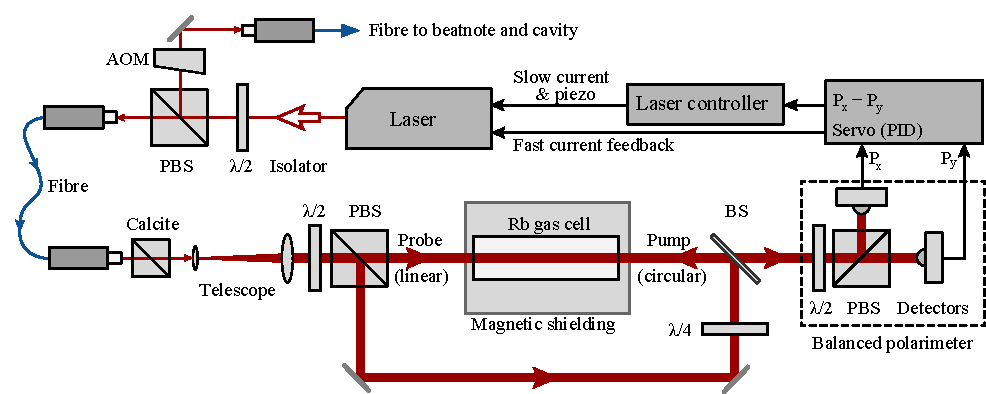
\includegraphics[width=\linewidth]{part1/Figs/ps_two_laser.pdf}
\caption{Schematic of the polarisation spectroscopy apparatus used to measure the performance of the high-bandwidth feedback. The beam from the laser passes through an isolator before being split into two beams by an \gls{pbs} and coupled into optical fibres.
One fibre leads to the \gls{ps} setup shown here, the other to the measurement apparatus via an \gls{aom}.
The \gls{ps} setup consists of a polarisation stabilising Glan-Thompson prism folled by a beam expanding telescope.
The expanded beam is then divided by a \gls{pbs} into a linearly polarised probe and circularly polarised pump which counter-propagate, via a non-polarising 50:50 \gls{bs}, through the magnetically-shielded \unit[15]{cm}-long rubidium gas sample.
The polarisation rotation of the probe beam is then measured by a balanced polarimeter which consists of a $\lambdaup/2$ waveplate, \gls{pbs} and two high-bandwidth photodetectors (Thorlabs PDA10A).}
\label{figure:two_laser_setup}
\end{figure}

A \unit[1]{GHz} detector\footnote{NewFocus 1621} was connected to a spectrum analyser\footnote{\unit[9]{kHz} to \unit[7]{KHz} Rohde and Swartz FSP7} to measure the spectrum of the beatnote that was centred around \unit[80]{MHz} due to the frequency shift imposed on one beam of the heterodyne measurement by an \gls{aom}.
An example of a beatnote from two lasers locked with \gls{ps} with high-bandwidth feedback is shown in Figure~\ref{figure:two_laser_beatnote}.
These measurements indicate that \gls{ps} with high-bandwidth feedback is able to narrow the laser linewidth to \unit[0.6$\pm$0.1]{kHz} which is significant improvement, two orders of magnitude, over previously published \gls{ps} performance~\cite{torii_laser-phase_2012}.

\begin{figure}
\center
%% Creator: Matplotlib, PGF backend
%%
%% To include the figure in your LaTeX document, write
%%   \input{<filename>.pgf}
%%
%% Make sure the required packages are loaded in your preamble
%%   \usepackage{pgf}
%%
%% Figures using additional raster images can only be included by \input if
%% they are in the same directory as the main LaTeX file. For loading figures
%% from other directories you can use the `import` package
%%   \usepackage{import}
%% and then include the figures with
%%   \import{<path to file>}{<filename>.pgf}
%%
%% Matplotlib used the following preamble
%%
\begingroup%
\makeatletter%
\begin{pgfpicture}%
\pgfpathrectangle{\pgfpointorigin}{\pgfqpoint{5.710000in}{3.172222in}}%
\pgfusepath{use as bounding box, clip}%
\begin{pgfscope}%
\pgfsetbuttcap%
\pgfsetmiterjoin%
\definecolor{currentfill}{rgb}{1.000000,1.000000,1.000000}%
\pgfsetfillcolor{currentfill}%
\pgfsetlinewidth{0.000000pt}%
\definecolor{currentstroke}{rgb}{1.000000,1.000000,1.000000}%
\pgfsetstrokecolor{currentstroke}%
\pgfsetdash{}{0pt}%
\pgfpathmoveto{\pgfqpoint{0.000000in}{0.000000in}}%
\pgfpathlineto{\pgfqpoint{5.710000in}{0.000000in}}%
\pgfpathlineto{\pgfqpoint{5.710000in}{3.172222in}}%
\pgfpathlineto{\pgfqpoint{0.000000in}{3.172222in}}%
\pgfpathclose%
\pgfusepath{fill}%
\end{pgfscope}%
\begin{pgfscope}%
\pgfsetbuttcap%
\pgfsetmiterjoin%
\definecolor{currentfill}{rgb}{1.000000,1.000000,1.000000}%
\pgfsetfillcolor{currentfill}%
\pgfsetlinewidth{0.000000pt}%
\definecolor{currentstroke}{rgb}{0.000000,0.000000,0.000000}%
\pgfsetstrokecolor{currentstroke}%
\pgfsetstrokeopacity{0.000000}%
\pgfsetdash{}{0pt}%
\pgfpathmoveto{\pgfqpoint{0.693845in}{0.521851in}}%
\pgfpathlineto{\pgfqpoint{5.560000in}{0.521851in}}%
\pgfpathlineto{\pgfqpoint{5.560000in}{3.022222in}}%
\pgfpathlineto{\pgfqpoint{0.693845in}{3.022222in}}%
\pgfpathclose%
\pgfusepath{fill}%
\end{pgfscope}%
\begin{pgfscope}%
\pgfpathrectangle{\pgfqpoint{0.693845in}{0.521851in}}{\pgfqpoint{4.866155in}{2.500371in}} %
\pgfusepath{clip}%
\pgfsetrectcap%
\pgfsetroundjoin%
\pgfsetlinewidth{0.501875pt}%
\definecolor{currentstroke}{rgb}{0.309804,0.478431,0.682353}%
\pgfsetstrokecolor{currentstroke}%
\pgfsetdash{}{0pt}%
\pgfpathmoveto{\pgfqpoint{0.693845in}{0.742508in}}%
\pgfpathlineto{\pgfqpoint{0.703578in}{0.686945in}}%
\pgfpathlineto{\pgfqpoint{0.713310in}{0.643348in}}%
\pgfpathlineto{\pgfqpoint{0.723042in}{0.675389in}}%
\pgfpathlineto{\pgfqpoint{0.732775in}{0.618502in}}%
\pgfpathlineto{\pgfqpoint{0.742507in}{0.585744in}}%
\pgfpathlineto{\pgfqpoint{0.752239in}{0.645516in}}%
\pgfpathlineto{\pgfqpoint{0.761972in}{0.673907in}}%
\pgfpathlineto{\pgfqpoint{0.771704in}{0.639132in}}%
\pgfpathlineto{\pgfqpoint{0.781436in}{0.628418in}}%
\pgfpathlineto{\pgfqpoint{0.791169in}{0.646413in}}%
\pgfpathlineto{\pgfqpoint{0.800901in}{0.752636in}}%
\pgfpathlineto{\pgfqpoint{0.810633in}{0.705751in}}%
\pgfpathlineto{\pgfqpoint{0.820365in}{0.648837in}}%
\pgfpathlineto{\pgfqpoint{0.830098in}{0.671328in}}%
\pgfpathlineto{\pgfqpoint{0.839830in}{0.669571in}}%
\pgfpathlineto{\pgfqpoint{0.849562in}{0.672274in}}%
\pgfpathlineto{\pgfqpoint{0.859295in}{0.680647in}}%
\pgfpathlineto{\pgfqpoint{0.869027in}{0.735591in}}%
\pgfpathlineto{\pgfqpoint{0.888492in}{0.677940in}}%
\pgfpathlineto{\pgfqpoint{0.898224in}{0.708509in}}%
\pgfpathlineto{\pgfqpoint{0.907956in}{0.708410in}}%
\pgfpathlineto{\pgfqpoint{0.917689in}{0.723481in}}%
\pgfpathlineto{\pgfqpoint{0.927421in}{0.663388in}}%
\pgfpathlineto{\pgfqpoint{0.937153in}{0.666497in}}%
\pgfpathlineto{\pgfqpoint{0.946885in}{0.640071in}}%
\pgfpathlineto{\pgfqpoint{0.956618in}{0.679513in}}%
\pgfpathlineto{\pgfqpoint{0.966350in}{0.680459in}}%
\pgfpathlineto{\pgfqpoint{0.985815in}{0.716882in}}%
\pgfpathlineto{\pgfqpoint{1.005279in}{0.691753in}}%
\pgfpathlineto{\pgfqpoint{1.015012in}{0.634913in}}%
\pgfpathlineto{\pgfqpoint{1.024744in}{0.652707in}}%
\pgfpathlineto{\pgfqpoint{1.034476in}{0.685421in}}%
\pgfpathlineto{\pgfqpoint{1.044209in}{0.646096in}}%
\pgfpathlineto{\pgfqpoint{1.053941in}{0.653909in}}%
\pgfpathlineto{\pgfqpoint{1.063673in}{0.612811in}}%
\pgfpathlineto{\pgfqpoint{1.073405in}{0.675480in}}%
\pgfpathlineto{\pgfqpoint{1.083138in}{0.706533in}}%
\pgfpathlineto{\pgfqpoint{1.092870in}{0.674091in}}%
\pgfpathlineto{\pgfqpoint{1.102602in}{0.647094in}}%
\pgfpathlineto{\pgfqpoint{1.112335in}{0.665702in}}%
\pgfpathlineto{\pgfqpoint{1.122067in}{0.676647in}}%
\pgfpathlineto{\pgfqpoint{1.131799in}{0.678914in}}%
\pgfpathlineto{\pgfqpoint{1.141532in}{0.694413in}}%
\pgfpathlineto{\pgfqpoint{1.151264in}{0.687945in}}%
\pgfpathlineto{\pgfqpoint{1.160996in}{0.697751in}}%
\pgfpathlineto{\pgfqpoint{1.170729in}{0.699702in}}%
\pgfpathlineto{\pgfqpoint{1.180461in}{0.748697in}}%
\pgfpathlineto{\pgfqpoint{1.190193in}{0.659300in}}%
\pgfpathlineto{\pgfqpoint{1.199925in}{0.707732in}}%
\pgfpathlineto{\pgfqpoint{1.209658in}{0.720242in}}%
\pgfpathlineto{\pgfqpoint{1.229122in}{0.681870in}}%
\pgfpathlineto{\pgfqpoint{1.238855in}{0.681975in}}%
\pgfpathlineto{\pgfqpoint{1.248587in}{0.731848in}}%
\pgfpathlineto{\pgfqpoint{1.258319in}{0.713909in}}%
\pgfpathlineto{\pgfqpoint{1.268052in}{0.675288in}}%
\pgfpathlineto{\pgfqpoint{1.277784in}{0.723084in}}%
\pgfpathlineto{\pgfqpoint{1.287516in}{0.718930in}}%
\pgfpathlineto{\pgfqpoint{1.297249in}{0.710043in}}%
\pgfpathlineto{\pgfqpoint{1.306981in}{0.761852in}}%
\pgfpathlineto{\pgfqpoint{1.316713in}{0.751098in}}%
\pgfpathlineto{\pgfqpoint{1.326446in}{0.760026in}}%
\pgfpathlineto{\pgfqpoint{1.336178in}{0.729347in}}%
\pgfpathlineto{\pgfqpoint{1.345910in}{0.727214in}}%
\pgfpathlineto{\pgfqpoint{1.355642in}{0.734269in}}%
\pgfpathlineto{\pgfqpoint{1.365375in}{0.708050in}}%
\pgfpathlineto{\pgfqpoint{1.375107in}{0.730271in}}%
\pgfpathlineto{\pgfqpoint{1.394572in}{0.744591in}}%
\pgfpathlineto{\pgfqpoint{1.404304in}{0.758455in}}%
\pgfpathlineto{\pgfqpoint{1.414036in}{0.701008in}}%
\pgfpathlineto{\pgfqpoint{1.423769in}{0.681611in}}%
\pgfpathlineto{\pgfqpoint{1.443233in}{0.731546in}}%
\pgfpathlineto{\pgfqpoint{1.452966in}{0.724646in}}%
\pgfpathlineto{\pgfqpoint{1.462698in}{0.757911in}}%
\pgfpathlineto{\pgfqpoint{1.472430in}{0.729338in}}%
\pgfpathlineto{\pgfqpoint{1.482162in}{0.786613in}}%
\pgfpathlineto{\pgfqpoint{1.491895in}{0.753978in}}%
\pgfpathlineto{\pgfqpoint{1.501627in}{0.761779in}}%
\pgfpathlineto{\pgfqpoint{1.511359in}{0.782788in}}%
\pgfpathlineto{\pgfqpoint{1.521092in}{0.788432in}}%
\pgfpathlineto{\pgfqpoint{1.530824in}{0.759161in}}%
\pgfpathlineto{\pgfqpoint{1.540556in}{0.747812in}}%
\pgfpathlineto{\pgfqpoint{1.550289in}{0.719772in}}%
\pgfpathlineto{\pgfqpoint{1.560021in}{0.767519in}}%
\pgfpathlineto{\pgfqpoint{1.569753in}{0.798183in}}%
\pgfpathlineto{\pgfqpoint{1.579486in}{0.770678in}}%
\pgfpathlineto{\pgfqpoint{1.589218in}{0.793431in}}%
\pgfpathlineto{\pgfqpoint{1.598950in}{0.812069in}}%
\pgfpathlineto{\pgfqpoint{1.608682in}{0.818105in}}%
\pgfpathlineto{\pgfqpoint{1.618415in}{0.773362in}}%
\pgfpathlineto{\pgfqpoint{1.628147in}{0.847068in}}%
\pgfpathlineto{\pgfqpoint{1.637879in}{0.841573in}}%
\pgfpathlineto{\pgfqpoint{1.647612in}{0.781970in}}%
\pgfpathlineto{\pgfqpoint{1.657344in}{0.750777in}}%
\pgfpathlineto{\pgfqpoint{1.667076in}{0.779774in}}%
\pgfpathlineto{\pgfqpoint{1.676809in}{0.859154in}}%
\pgfpathlineto{\pgfqpoint{1.686541in}{0.869605in}}%
\pgfpathlineto{\pgfqpoint{1.696273in}{0.836882in}}%
\pgfpathlineto{\pgfqpoint{1.706006in}{0.845689in}}%
\pgfpathlineto{\pgfqpoint{1.715738in}{0.840907in}}%
\pgfpathlineto{\pgfqpoint{1.725470in}{0.825145in}}%
\pgfpathlineto{\pgfqpoint{1.735203in}{0.885424in}}%
\pgfpathlineto{\pgfqpoint{1.744935in}{0.915001in}}%
\pgfpathlineto{\pgfqpoint{1.754667in}{0.841018in}}%
\pgfpathlineto{\pgfqpoint{1.764399in}{0.853648in}}%
\pgfpathlineto{\pgfqpoint{1.774132in}{0.890396in}}%
\pgfpathlineto{\pgfqpoint{1.783864in}{0.845387in}}%
\pgfpathlineto{\pgfqpoint{1.793596in}{0.875251in}}%
\pgfpathlineto{\pgfqpoint{1.813061in}{0.957338in}}%
\pgfpathlineto{\pgfqpoint{1.822793in}{0.945061in}}%
\pgfpathlineto{\pgfqpoint{1.832526in}{0.874159in}}%
\pgfpathlineto{\pgfqpoint{1.842258in}{0.908167in}}%
\pgfpathlineto{\pgfqpoint{1.851990in}{0.873342in}}%
\pgfpathlineto{\pgfqpoint{1.861723in}{0.875805in}}%
\pgfpathlineto{\pgfqpoint{1.871455in}{0.843316in}}%
\pgfpathlineto{\pgfqpoint{1.881187in}{0.879710in}}%
\pgfpathlineto{\pgfqpoint{1.890919in}{0.964634in}}%
\pgfpathlineto{\pgfqpoint{1.900652in}{0.923598in}}%
\pgfpathlineto{\pgfqpoint{1.910384in}{0.912187in}}%
\pgfpathlineto{\pgfqpoint{1.920116in}{0.908568in}}%
\pgfpathlineto{\pgfqpoint{1.929849in}{0.894379in}}%
\pgfpathlineto{\pgfqpoint{1.939581in}{1.002769in}}%
\pgfpathlineto{\pgfqpoint{1.949313in}{1.017998in}}%
\pgfpathlineto{\pgfqpoint{1.959046in}{0.986589in}}%
\pgfpathlineto{\pgfqpoint{1.968778in}{0.939933in}}%
\pgfpathlineto{\pgfqpoint{1.978510in}{0.947193in}}%
\pgfpathlineto{\pgfqpoint{1.988243in}{0.990964in}}%
\pgfpathlineto{\pgfqpoint{1.997975in}{0.989175in}}%
\pgfpathlineto{\pgfqpoint{2.007707in}{0.986016in}}%
\pgfpathlineto{\pgfqpoint{2.017439in}{0.992098in}}%
\pgfpathlineto{\pgfqpoint{2.027172in}{0.985130in}}%
\pgfpathlineto{\pgfqpoint{2.036904in}{1.027719in}}%
\pgfpathlineto{\pgfqpoint{2.046636in}{1.020592in}}%
\pgfpathlineto{\pgfqpoint{2.056369in}{1.004902in}}%
\pgfpathlineto{\pgfqpoint{2.066101in}{0.993746in}}%
\pgfpathlineto{\pgfqpoint{2.075833in}{1.023446in}}%
\pgfpathlineto{\pgfqpoint{2.085566in}{0.986362in}}%
\pgfpathlineto{\pgfqpoint{2.095298in}{1.017895in}}%
\pgfpathlineto{\pgfqpoint{2.105030in}{0.989159in}}%
\pgfpathlineto{\pgfqpoint{2.114763in}{1.042564in}}%
\pgfpathlineto{\pgfqpoint{2.124495in}{1.049863in}}%
\pgfpathlineto{\pgfqpoint{2.134227in}{1.042788in}}%
\pgfpathlineto{\pgfqpoint{2.143959in}{1.052786in}}%
\pgfpathlineto{\pgfqpoint{2.153692in}{1.047990in}}%
\pgfpathlineto{\pgfqpoint{2.163424in}{1.001308in}}%
\pgfpathlineto{\pgfqpoint{2.173156in}{1.039855in}}%
\pgfpathlineto{\pgfqpoint{2.182889in}{1.005467in}}%
\pgfpathlineto{\pgfqpoint{2.192621in}{1.107555in}}%
\pgfpathlineto{\pgfqpoint{2.202353in}{1.071186in}}%
\pgfpathlineto{\pgfqpoint{2.212086in}{1.081797in}}%
\pgfpathlineto{\pgfqpoint{2.221818in}{1.115454in}}%
\pgfpathlineto{\pgfqpoint{2.231550in}{1.138752in}}%
\pgfpathlineto{\pgfqpoint{2.241283in}{1.110022in}}%
\pgfpathlineto{\pgfqpoint{2.251015in}{1.119364in}}%
\pgfpathlineto{\pgfqpoint{2.260747in}{1.108872in}}%
\pgfpathlineto{\pgfqpoint{2.270480in}{1.121364in}}%
\pgfpathlineto{\pgfqpoint{2.280212in}{1.157153in}}%
\pgfpathlineto{\pgfqpoint{2.289944in}{1.152908in}}%
\pgfpathlineto{\pgfqpoint{2.299676in}{1.210562in}}%
\pgfpathlineto{\pgfqpoint{2.309409in}{1.241699in}}%
\pgfpathlineto{\pgfqpoint{2.319141in}{1.195631in}}%
\pgfpathlineto{\pgfqpoint{2.328873in}{1.266763in}}%
\pgfpathlineto{\pgfqpoint{2.338606in}{1.311553in}}%
\pgfpathlineto{\pgfqpoint{2.348338in}{1.339449in}}%
\pgfpathlineto{\pgfqpoint{2.358070in}{1.274047in}}%
\pgfpathlineto{\pgfqpoint{2.367803in}{1.283029in}}%
\pgfpathlineto{\pgfqpoint{2.377535in}{1.342425in}}%
\pgfpathlineto{\pgfqpoint{2.387267in}{1.322655in}}%
\pgfpathlineto{\pgfqpoint{2.397000in}{1.310510in}}%
\pgfpathlineto{\pgfqpoint{2.406732in}{1.322265in}}%
\pgfpathlineto{\pgfqpoint{2.416464in}{1.368756in}}%
\pgfpathlineto{\pgfqpoint{2.426196in}{1.388692in}}%
\pgfpathlineto{\pgfqpoint{2.435929in}{1.341120in}}%
\pgfpathlineto{\pgfqpoint{2.445661in}{1.340602in}}%
\pgfpathlineto{\pgfqpoint{2.455393in}{1.461022in}}%
\pgfpathlineto{\pgfqpoint{2.465126in}{1.481205in}}%
\pgfpathlineto{\pgfqpoint{2.474858in}{1.444994in}}%
\pgfpathlineto{\pgfqpoint{2.484590in}{1.472483in}}%
\pgfpathlineto{\pgfqpoint{2.494323in}{1.503366in}}%
\pgfpathlineto{\pgfqpoint{2.504055in}{1.478162in}}%
\pgfpathlineto{\pgfqpoint{2.513787in}{1.476998in}}%
\pgfpathlineto{\pgfqpoint{2.523520in}{1.484148in}}%
\pgfpathlineto{\pgfqpoint{2.533252in}{1.480387in}}%
\pgfpathlineto{\pgfqpoint{2.542984in}{1.560208in}}%
\pgfpathlineto{\pgfqpoint{2.552716in}{1.518771in}}%
\pgfpathlineto{\pgfqpoint{2.562449in}{1.532182in}}%
\pgfpathlineto{\pgfqpoint{2.572181in}{1.540143in}}%
\pgfpathlineto{\pgfqpoint{2.581913in}{1.543604in}}%
\pgfpathlineto{\pgfqpoint{2.591646in}{1.543298in}}%
\pgfpathlineto{\pgfqpoint{2.601378in}{1.460801in}}%
\pgfpathlineto{\pgfqpoint{2.611110in}{1.507432in}}%
\pgfpathlineto{\pgfqpoint{2.620843in}{1.532024in}}%
\pgfpathlineto{\pgfqpoint{2.630575in}{1.553002in}}%
\pgfpathlineto{\pgfqpoint{2.650040in}{1.574542in}}%
\pgfpathlineto{\pgfqpoint{2.659772in}{1.570973in}}%
\pgfpathlineto{\pgfqpoint{2.669504in}{1.533347in}}%
\pgfpathlineto{\pgfqpoint{2.679236in}{1.578440in}}%
\pgfpathlineto{\pgfqpoint{2.688969in}{1.611749in}}%
\pgfpathlineto{\pgfqpoint{2.698701in}{1.629500in}}%
\pgfpathlineto{\pgfqpoint{2.708433in}{1.569703in}}%
\pgfpathlineto{\pgfqpoint{2.718166in}{1.554476in}}%
\pgfpathlineto{\pgfqpoint{2.727898in}{1.536838in}}%
\pgfpathlineto{\pgfqpoint{2.737630in}{1.564810in}}%
\pgfpathlineto{\pgfqpoint{2.747363in}{1.652080in}}%
\pgfpathlineto{\pgfqpoint{2.766827in}{1.591134in}}%
\pgfpathlineto{\pgfqpoint{2.776560in}{1.653786in}}%
\pgfpathlineto{\pgfqpoint{2.786292in}{1.663975in}}%
\pgfpathlineto{\pgfqpoint{2.796024in}{1.553504in}}%
\pgfpathlineto{\pgfqpoint{2.805757in}{1.555208in}}%
\pgfpathlineto{\pgfqpoint{2.815489in}{1.497077in}}%
\pgfpathlineto{\pgfqpoint{2.825221in}{1.595506in}}%
\pgfpathlineto{\pgfqpoint{2.834953in}{1.620996in}}%
\pgfpathlineto{\pgfqpoint{2.844686in}{1.679087in}}%
\pgfpathlineto{\pgfqpoint{2.854418in}{1.728648in}}%
\pgfpathlineto{\pgfqpoint{2.873883in}{1.626743in}}%
\pgfpathlineto{\pgfqpoint{2.883615in}{1.599582in}}%
\pgfpathlineto{\pgfqpoint{2.893347in}{1.658113in}}%
\pgfpathlineto{\pgfqpoint{2.903080in}{1.652476in}}%
\pgfpathlineto{\pgfqpoint{2.912812in}{1.580381in}}%
\pgfpathlineto{\pgfqpoint{2.922544in}{1.603869in}}%
\pgfpathlineto{\pgfqpoint{2.932277in}{1.707493in}}%
\pgfpathlineto{\pgfqpoint{2.942009in}{1.554309in}}%
\pgfpathlineto{\pgfqpoint{2.951741in}{1.614609in}}%
\pgfpathlineto{\pgfqpoint{2.961473in}{1.549327in}}%
\pgfpathlineto{\pgfqpoint{2.971206in}{1.597993in}}%
\pgfpathlineto{\pgfqpoint{2.990670in}{1.649636in}}%
\pgfpathlineto{\pgfqpoint{3.000403in}{1.713888in}}%
\pgfpathlineto{\pgfqpoint{3.010135in}{1.688093in}}%
\pgfpathlineto{\pgfqpoint{3.019867in}{1.653968in}}%
\pgfpathlineto{\pgfqpoint{3.029600in}{1.682611in}}%
\pgfpathlineto{\pgfqpoint{3.039332in}{1.769926in}}%
\pgfpathlineto{\pgfqpoint{3.049064in}{1.835601in}}%
\pgfpathlineto{\pgfqpoint{3.058797in}{1.829224in}}%
\pgfpathlineto{\pgfqpoint{3.068529in}{1.839555in}}%
\pgfpathlineto{\pgfqpoint{3.078261in}{1.838211in}}%
\pgfpathlineto{\pgfqpoint{3.097726in}{1.739283in}}%
\pgfpathlineto{\pgfqpoint{3.107458in}{1.758120in}}%
\pgfpathlineto{\pgfqpoint{3.117190in}{1.748329in}}%
\pgfpathlineto{\pgfqpoint{3.126923in}{1.634130in}}%
\pgfpathlineto{\pgfqpoint{3.136655in}{1.594527in}}%
\pgfpathlineto{\pgfqpoint{3.146387in}{1.575812in}}%
\pgfpathlineto{\pgfqpoint{3.156120in}{1.582822in}}%
\pgfpathlineto{\pgfqpoint{3.165852in}{1.521502in}}%
\pgfpathlineto{\pgfqpoint{3.175584in}{1.539036in}}%
\pgfpathlineto{\pgfqpoint{3.185317in}{1.624620in}}%
\pgfpathlineto{\pgfqpoint{3.195049in}{1.631775in}}%
\pgfpathlineto{\pgfqpoint{3.204781in}{2.155184in}}%
\pgfpathlineto{\pgfqpoint{3.214513in}{2.867502in}}%
\pgfpathlineto{\pgfqpoint{3.224246in}{2.788733in}}%
\pgfpathlineto{\pgfqpoint{3.233978in}{1.658783in}}%
\pgfpathlineto{\pgfqpoint{3.243710in}{1.503068in}}%
\pgfpathlineto{\pgfqpoint{3.253443in}{1.490172in}}%
\pgfpathlineto{\pgfqpoint{3.263175in}{1.495874in}}%
\pgfpathlineto{\pgfqpoint{3.272907in}{1.505208in}}%
\pgfpathlineto{\pgfqpoint{3.282640in}{1.561176in}}%
\pgfpathlineto{\pgfqpoint{3.292372in}{1.604269in}}%
\pgfpathlineto{\pgfqpoint{3.302104in}{1.595189in}}%
\pgfpathlineto{\pgfqpoint{3.311837in}{1.636564in}}%
\pgfpathlineto{\pgfqpoint{3.321569in}{1.739985in}}%
\pgfpathlineto{\pgfqpoint{3.331301in}{1.740396in}}%
\pgfpathlineto{\pgfqpoint{3.341034in}{1.785857in}}%
\pgfpathlineto{\pgfqpoint{3.350766in}{1.754698in}}%
\pgfpathlineto{\pgfqpoint{3.360498in}{1.812656in}}%
\pgfpathlineto{\pgfqpoint{3.370230in}{1.849726in}}%
\pgfpathlineto{\pgfqpoint{3.379963in}{1.748257in}}%
\pgfpathlineto{\pgfqpoint{3.389695in}{1.742174in}}%
\pgfpathlineto{\pgfqpoint{3.399427in}{1.769695in}}%
\pgfpathlineto{\pgfqpoint{3.409160in}{1.741000in}}%
\pgfpathlineto{\pgfqpoint{3.418892in}{1.692563in}}%
\pgfpathlineto{\pgfqpoint{3.428624in}{1.752587in}}%
\pgfpathlineto{\pgfqpoint{3.438357in}{1.717356in}}%
\pgfpathlineto{\pgfqpoint{3.448089in}{1.701752in}}%
\pgfpathlineto{\pgfqpoint{3.457821in}{1.672544in}}%
\pgfpathlineto{\pgfqpoint{3.467554in}{1.636766in}}%
\pgfpathlineto{\pgfqpoint{3.477286in}{1.694648in}}%
\pgfpathlineto{\pgfqpoint{3.496750in}{1.569386in}}%
\pgfpathlineto{\pgfqpoint{3.506483in}{1.467670in}}%
\pgfpathlineto{\pgfqpoint{3.516215in}{1.544632in}}%
\pgfpathlineto{\pgfqpoint{3.525947in}{1.582459in}}%
\pgfpathlineto{\pgfqpoint{3.535680in}{1.611230in}}%
\pgfpathlineto{\pgfqpoint{3.545412in}{1.570439in}}%
\pgfpathlineto{\pgfqpoint{3.555144in}{1.536813in}}%
\pgfpathlineto{\pgfqpoint{3.564877in}{1.546893in}}%
\pgfpathlineto{\pgfqpoint{3.574609in}{1.543741in}}%
\pgfpathlineto{\pgfqpoint{3.584341in}{1.515836in}}%
\pgfpathlineto{\pgfqpoint{3.594074in}{1.470756in}}%
\pgfpathlineto{\pgfqpoint{3.603806in}{1.466696in}}%
\pgfpathlineto{\pgfqpoint{3.613538in}{1.540911in}}%
\pgfpathlineto{\pgfqpoint{3.623270in}{1.563831in}}%
\pgfpathlineto{\pgfqpoint{3.633003in}{1.559181in}}%
\pgfpathlineto{\pgfqpoint{3.642735in}{1.603146in}}%
\pgfpathlineto{\pgfqpoint{3.652467in}{1.566057in}}%
\pgfpathlineto{\pgfqpoint{3.662200in}{1.491586in}}%
\pgfpathlineto{\pgfqpoint{3.671932in}{1.493762in}}%
\pgfpathlineto{\pgfqpoint{3.681664in}{1.522288in}}%
\pgfpathlineto{\pgfqpoint{3.691397in}{1.562475in}}%
\pgfpathlineto{\pgfqpoint{3.701129in}{1.528719in}}%
\pgfpathlineto{\pgfqpoint{3.710861in}{1.482401in}}%
\pgfpathlineto{\pgfqpoint{3.720594in}{1.544405in}}%
\pgfpathlineto{\pgfqpoint{3.730326in}{1.597530in}}%
\pgfpathlineto{\pgfqpoint{3.740058in}{1.565141in}}%
\pgfpathlineto{\pgfqpoint{3.749790in}{1.631836in}}%
\pgfpathlineto{\pgfqpoint{3.759523in}{1.639847in}}%
\pgfpathlineto{\pgfqpoint{3.769255in}{1.645127in}}%
\pgfpathlineto{\pgfqpoint{3.778987in}{1.557583in}}%
\pgfpathlineto{\pgfqpoint{3.788720in}{1.540563in}}%
\pgfpathlineto{\pgfqpoint{3.798452in}{1.543764in}}%
\pgfpathlineto{\pgfqpoint{3.808184in}{1.618155in}}%
\pgfpathlineto{\pgfqpoint{3.817917in}{1.540939in}}%
\pgfpathlineto{\pgfqpoint{3.827649in}{1.557928in}}%
\pgfpathlineto{\pgfqpoint{3.837381in}{1.543742in}}%
\pgfpathlineto{\pgfqpoint{3.847114in}{1.535389in}}%
\pgfpathlineto{\pgfqpoint{3.856846in}{1.483124in}}%
\pgfpathlineto{\pgfqpoint{3.866578in}{1.455826in}}%
\pgfpathlineto{\pgfqpoint{3.876311in}{1.470870in}}%
\pgfpathlineto{\pgfqpoint{3.886043in}{1.515900in}}%
\pgfpathlineto{\pgfqpoint{3.895775in}{1.472746in}}%
\pgfpathlineto{\pgfqpoint{3.905507in}{1.528438in}}%
\pgfpathlineto{\pgfqpoint{3.915240in}{1.470644in}}%
\pgfpathlineto{\pgfqpoint{3.924972in}{1.469592in}}%
\pgfpathlineto{\pgfqpoint{3.934704in}{1.415540in}}%
\pgfpathlineto{\pgfqpoint{3.944437in}{1.452254in}}%
\pgfpathlineto{\pgfqpoint{3.963901in}{1.416501in}}%
\pgfpathlineto{\pgfqpoint{3.973634in}{1.391819in}}%
\pgfpathlineto{\pgfqpoint{3.983366in}{1.333232in}}%
\pgfpathlineto{\pgfqpoint{3.993098in}{1.381837in}}%
\pgfpathlineto{\pgfqpoint{4.002831in}{1.385596in}}%
\pgfpathlineto{\pgfqpoint{4.012563in}{1.319685in}}%
\pgfpathlineto{\pgfqpoint{4.022295in}{1.322735in}}%
\pgfpathlineto{\pgfqpoint{4.032027in}{1.291677in}}%
\pgfpathlineto{\pgfqpoint{4.041760in}{1.371994in}}%
\pgfpathlineto{\pgfqpoint{4.051492in}{1.320200in}}%
\pgfpathlineto{\pgfqpoint{4.061224in}{1.309998in}}%
\pgfpathlineto{\pgfqpoint{4.070957in}{1.325557in}}%
\pgfpathlineto{\pgfqpoint{4.080689in}{1.323850in}}%
\pgfpathlineto{\pgfqpoint{4.090421in}{1.246969in}}%
\pgfpathlineto{\pgfqpoint{4.100154in}{1.245468in}}%
\pgfpathlineto{\pgfqpoint{4.109886in}{1.218853in}}%
\pgfpathlineto{\pgfqpoint{4.119618in}{1.179336in}}%
\pgfpathlineto{\pgfqpoint{4.129351in}{1.229822in}}%
\pgfpathlineto{\pgfqpoint{4.139083in}{1.230265in}}%
\pgfpathlineto{\pgfqpoint{4.148815in}{1.163838in}}%
\pgfpathlineto{\pgfqpoint{4.158547in}{1.171112in}}%
\pgfpathlineto{\pgfqpoint{4.168280in}{1.110314in}}%
\pgfpathlineto{\pgfqpoint{4.178012in}{1.091251in}}%
\pgfpathlineto{\pgfqpoint{4.187744in}{1.119352in}}%
\pgfpathlineto{\pgfqpoint{4.197477in}{1.031128in}}%
\pgfpathlineto{\pgfqpoint{4.207209in}{1.066817in}}%
\pgfpathlineto{\pgfqpoint{4.216941in}{1.062599in}}%
\pgfpathlineto{\pgfqpoint{4.226674in}{1.056683in}}%
\pgfpathlineto{\pgfqpoint{4.236406in}{1.089556in}}%
\pgfpathlineto{\pgfqpoint{4.246138in}{1.048928in}}%
\pgfpathlineto{\pgfqpoint{4.255871in}{1.019089in}}%
\pgfpathlineto{\pgfqpoint{4.265603in}{1.036286in}}%
\pgfpathlineto{\pgfqpoint{4.275335in}{1.013704in}}%
\pgfpathlineto{\pgfqpoint{4.285068in}{1.037738in}}%
\pgfpathlineto{\pgfqpoint{4.294800in}{1.050643in}}%
\pgfpathlineto{\pgfqpoint{4.304532in}{1.077198in}}%
\pgfpathlineto{\pgfqpoint{4.314264in}{1.043968in}}%
\pgfpathlineto{\pgfqpoint{4.323997in}{1.092920in}}%
\pgfpathlineto{\pgfqpoint{4.333729in}{1.038418in}}%
\pgfpathlineto{\pgfqpoint{4.343461in}{0.996275in}}%
\pgfpathlineto{\pgfqpoint{4.353194in}{1.028824in}}%
\pgfpathlineto{\pgfqpoint{4.362926in}{0.983369in}}%
\pgfpathlineto{\pgfqpoint{4.372658in}{0.966630in}}%
\pgfpathlineto{\pgfqpoint{4.382391in}{0.966315in}}%
\pgfpathlineto{\pgfqpoint{4.392123in}{0.946221in}}%
\pgfpathlineto{\pgfqpoint{4.401855in}{1.007266in}}%
\pgfpathlineto{\pgfqpoint{4.411588in}{0.963181in}}%
\pgfpathlineto{\pgfqpoint{4.421320in}{0.885970in}}%
\pgfpathlineto{\pgfqpoint{4.431052in}{0.973252in}}%
\pgfpathlineto{\pgfqpoint{4.440784in}{1.013670in}}%
\pgfpathlineto{\pgfqpoint{4.450517in}{0.958451in}}%
\pgfpathlineto{\pgfqpoint{4.460249in}{0.982078in}}%
\pgfpathlineto{\pgfqpoint{4.469981in}{0.928401in}}%
\pgfpathlineto{\pgfqpoint{4.479714in}{0.937103in}}%
\pgfpathlineto{\pgfqpoint{4.489446in}{0.883294in}}%
\pgfpathlineto{\pgfqpoint{4.499178in}{0.897197in}}%
\pgfpathlineto{\pgfqpoint{4.508911in}{0.977094in}}%
\pgfpathlineto{\pgfqpoint{4.528375in}{0.868518in}}%
\pgfpathlineto{\pgfqpoint{4.538108in}{0.854361in}}%
\pgfpathlineto{\pgfqpoint{4.547840in}{0.886133in}}%
\pgfpathlineto{\pgfqpoint{4.557572in}{0.893499in}}%
\pgfpathlineto{\pgfqpoint{4.567304in}{0.859799in}}%
\pgfpathlineto{\pgfqpoint{4.577037in}{0.891007in}}%
\pgfpathlineto{\pgfqpoint{4.586769in}{0.885777in}}%
\pgfpathlineto{\pgfqpoint{4.596501in}{0.853591in}}%
\pgfpathlineto{\pgfqpoint{4.606234in}{0.850466in}}%
\pgfpathlineto{\pgfqpoint{4.615966in}{0.875261in}}%
\pgfpathlineto{\pgfqpoint{4.625698in}{0.946409in}}%
\pgfpathlineto{\pgfqpoint{4.635431in}{0.835077in}}%
\pgfpathlineto{\pgfqpoint{4.645163in}{0.843841in}}%
\pgfpathlineto{\pgfqpoint{4.654895in}{0.858297in}}%
\pgfpathlineto{\pgfqpoint{4.664628in}{0.881161in}}%
\pgfpathlineto{\pgfqpoint{4.674360in}{0.874910in}}%
\pgfpathlineto{\pgfqpoint{4.684092in}{0.773499in}}%
\pgfpathlineto{\pgfqpoint{4.693824in}{0.842077in}}%
\pgfpathlineto{\pgfqpoint{4.703557in}{0.864682in}}%
\pgfpathlineto{\pgfqpoint{4.713289in}{0.816833in}}%
\pgfpathlineto{\pgfqpoint{4.723021in}{0.790000in}}%
\pgfpathlineto{\pgfqpoint{4.732754in}{0.814755in}}%
\pgfpathlineto{\pgfqpoint{4.742486in}{0.792704in}}%
\pgfpathlineto{\pgfqpoint{4.752218in}{0.820723in}}%
\pgfpathlineto{\pgfqpoint{4.761951in}{0.835495in}}%
\pgfpathlineto{\pgfqpoint{4.771683in}{0.780821in}}%
\pgfpathlineto{\pgfqpoint{4.781415in}{0.779188in}}%
\pgfpathlineto{\pgfqpoint{4.791148in}{0.837156in}}%
\pgfpathlineto{\pgfqpoint{4.800880in}{0.823498in}}%
\pgfpathlineto{\pgfqpoint{4.810612in}{0.824977in}}%
\pgfpathlineto{\pgfqpoint{4.820345in}{0.770787in}}%
\pgfpathlineto{\pgfqpoint{4.830077in}{0.777994in}}%
\pgfpathlineto{\pgfqpoint{4.849541in}{0.815137in}}%
\pgfpathlineto{\pgfqpoint{4.859274in}{0.766047in}}%
\pgfpathlineto{\pgfqpoint{4.869006in}{0.745749in}}%
\pgfpathlineto{\pgfqpoint{4.878738in}{0.729096in}}%
\pgfpathlineto{\pgfqpoint{4.888471in}{0.809931in}}%
\pgfpathlineto{\pgfqpoint{4.898203in}{0.813684in}}%
\pgfpathlineto{\pgfqpoint{4.907935in}{0.767041in}}%
\pgfpathlineto{\pgfqpoint{4.917668in}{0.802339in}}%
\pgfpathlineto{\pgfqpoint{4.927400in}{0.751149in}}%
\pgfpathlineto{\pgfqpoint{4.937132in}{0.736737in}}%
\pgfpathlineto{\pgfqpoint{4.946865in}{0.739230in}}%
\pgfpathlineto{\pgfqpoint{4.956597in}{0.738633in}}%
\pgfpathlineto{\pgfqpoint{4.966329in}{0.688208in}}%
\pgfpathlineto{\pgfqpoint{4.976061in}{0.755892in}}%
\pgfpathlineto{\pgfqpoint{4.985794in}{0.737977in}}%
\pgfpathlineto{\pgfqpoint{4.995526in}{0.797296in}}%
\pgfpathlineto{\pgfqpoint{5.005258in}{0.791174in}}%
\pgfpathlineto{\pgfqpoint{5.014991in}{0.760323in}}%
\pgfpathlineto{\pgfqpoint{5.024723in}{0.751040in}}%
\pgfpathlineto{\pgfqpoint{5.034455in}{0.703038in}}%
\pgfpathlineto{\pgfqpoint{5.044188in}{0.708252in}}%
\pgfpathlineto{\pgfqpoint{5.053920in}{0.674494in}}%
\pgfpathlineto{\pgfqpoint{5.063652in}{0.722422in}}%
\pgfpathlineto{\pgfqpoint{5.073385in}{0.744695in}}%
\pgfpathlineto{\pgfqpoint{5.083117in}{0.737848in}}%
\pgfpathlineto{\pgfqpoint{5.092849in}{0.706980in}}%
\pgfpathlineto{\pgfqpoint{5.102581in}{0.701236in}}%
\pgfpathlineto{\pgfqpoint{5.112314in}{0.697382in}}%
\pgfpathlineto{\pgfqpoint{5.122046in}{0.739470in}}%
\pgfpathlineto{\pgfqpoint{5.131778in}{0.730548in}}%
\pgfpathlineto{\pgfqpoint{5.141511in}{0.739082in}}%
\pgfpathlineto{\pgfqpoint{5.151243in}{0.739357in}}%
\pgfpathlineto{\pgfqpoint{5.160975in}{0.697206in}}%
\pgfpathlineto{\pgfqpoint{5.170708in}{0.722298in}}%
\pgfpathlineto{\pgfqpoint{5.180440in}{0.725883in}}%
\pgfpathlineto{\pgfqpoint{5.190172in}{0.753316in}}%
\pgfpathlineto{\pgfqpoint{5.199905in}{0.698219in}}%
\pgfpathlineto{\pgfqpoint{5.219369in}{0.751151in}}%
\pgfpathlineto{\pgfqpoint{5.229101in}{0.700446in}}%
\pgfpathlineto{\pgfqpoint{5.238834in}{0.670737in}}%
\pgfpathlineto{\pgfqpoint{5.248566in}{0.731659in}}%
\pgfpathlineto{\pgfqpoint{5.258298in}{0.759890in}}%
\pgfpathlineto{\pgfqpoint{5.268031in}{0.762712in}}%
\pgfpathlineto{\pgfqpoint{5.277763in}{0.693701in}}%
\pgfpathlineto{\pgfqpoint{5.287495in}{0.746825in}}%
\pgfpathlineto{\pgfqpoint{5.297228in}{0.707944in}}%
\pgfpathlineto{\pgfqpoint{5.306960in}{0.712059in}}%
\pgfpathlineto{\pgfqpoint{5.316692in}{0.724257in}}%
\pgfpathlineto{\pgfqpoint{5.326425in}{0.673450in}}%
\pgfpathlineto{\pgfqpoint{5.345889in}{0.688274in}}%
\pgfpathlineto{\pgfqpoint{5.355622in}{0.670991in}}%
\pgfpathlineto{\pgfqpoint{5.365354in}{0.704533in}}%
\pgfpathlineto{\pgfqpoint{5.375086in}{0.713574in}}%
\pgfpathlineto{\pgfqpoint{5.384818in}{0.715439in}}%
\pgfpathlineto{\pgfqpoint{5.394551in}{0.690541in}}%
\pgfpathlineto{\pgfqpoint{5.404283in}{0.669148in}}%
\pgfpathlineto{\pgfqpoint{5.414015in}{0.688626in}}%
\pgfpathlineto{\pgfqpoint{5.423748in}{0.685945in}}%
\pgfpathlineto{\pgfqpoint{5.433480in}{0.717366in}}%
\pgfpathlineto{\pgfqpoint{5.443212in}{0.711669in}}%
\pgfpathlineto{\pgfqpoint{5.452945in}{0.647884in}}%
\pgfpathlineto{\pgfqpoint{5.462677in}{0.682121in}}%
\pgfpathlineto{\pgfqpoint{5.472409in}{0.725745in}}%
\pgfpathlineto{\pgfqpoint{5.482142in}{0.699858in}}%
\pgfpathlineto{\pgfqpoint{5.491874in}{0.726831in}}%
\pgfpathlineto{\pgfqpoint{5.501606in}{0.718152in}}%
\pgfpathlineto{\pgfqpoint{5.511338in}{0.644003in}}%
\pgfpathlineto{\pgfqpoint{5.521071in}{0.627610in}}%
\pgfpathlineto{\pgfqpoint{5.530803in}{0.650682in}}%
\pgfpathlineto{\pgfqpoint{5.540535in}{0.686696in}}%
\pgfpathlineto{\pgfqpoint{5.550268in}{0.693786in}}%
\pgfpathlineto{\pgfqpoint{5.560000in}{0.672916in}}%
\pgfpathlineto{\pgfqpoint{5.560000in}{0.672916in}}%
\pgfusepath{stroke}%
\end{pgfscope}%
\begin{pgfscope}%
\pgfsetrectcap%
\pgfsetmiterjoin%
\pgfsetlinewidth{1.003750pt}%
\definecolor{currentstroke}{rgb}{0.000000,0.000000,0.000000}%
\pgfsetstrokecolor{currentstroke}%
\pgfsetdash{}{0pt}%
\pgfpathmoveto{\pgfqpoint{0.693845in}{3.022222in}}%
\pgfpathlineto{\pgfqpoint{5.560000in}{3.022222in}}%
\pgfusepath{stroke}%
\end{pgfscope}%
\begin{pgfscope}%
\pgfsetrectcap%
\pgfsetmiterjoin%
\pgfsetlinewidth{1.003750pt}%
\definecolor{currentstroke}{rgb}{0.000000,0.000000,0.000000}%
\pgfsetstrokecolor{currentstroke}%
\pgfsetdash{}{0pt}%
\pgfpathmoveto{\pgfqpoint{5.560000in}{0.521851in}}%
\pgfpathlineto{\pgfqpoint{5.560000in}{3.022222in}}%
\pgfusepath{stroke}%
\end{pgfscope}%
\begin{pgfscope}%
\pgfsetrectcap%
\pgfsetmiterjoin%
\pgfsetlinewidth{1.003750pt}%
\definecolor{currentstroke}{rgb}{0.000000,0.000000,0.000000}%
\pgfsetstrokecolor{currentstroke}%
\pgfsetdash{}{0pt}%
\pgfpathmoveto{\pgfqpoint{0.693845in}{0.521851in}}%
\pgfpathlineto{\pgfqpoint{5.560000in}{0.521851in}}%
\pgfusepath{stroke}%
\end{pgfscope}%
\begin{pgfscope}%
\pgfsetrectcap%
\pgfsetmiterjoin%
\pgfsetlinewidth{1.003750pt}%
\definecolor{currentstroke}{rgb}{0.000000,0.000000,0.000000}%
\pgfsetstrokecolor{currentstroke}%
\pgfsetdash{}{0pt}%
\pgfpathmoveto{\pgfqpoint{0.693845in}{0.521851in}}%
\pgfpathlineto{\pgfqpoint{0.693845in}{3.022222in}}%
\pgfusepath{stroke}%
\end{pgfscope}%
\begin{pgfscope}%
\pgfsetbuttcap%
\pgfsetroundjoin%
\definecolor{currentfill}{rgb}{0.000000,0.000000,0.000000}%
\pgfsetfillcolor{currentfill}%
\pgfsetlinewidth{0.501875pt}%
\definecolor{currentstroke}{rgb}{0.000000,0.000000,0.000000}%
\pgfsetstrokecolor{currentstroke}%
\pgfsetdash{}{0pt}%
\pgfsys@defobject{currentmarker}{\pgfqpoint{0.000000in}{0.000000in}}{\pgfqpoint{0.000000in}{0.055556in}}{%
\pgfpathmoveto{\pgfqpoint{0.000000in}{0.000000in}}%
\pgfpathlineto{\pgfqpoint{0.000000in}{0.055556in}}%
\pgfusepath{stroke,fill}%
}%
\begin{pgfscope}%
\pgfsys@transformshift{1.268052in}{0.521851in}%
\pgfsys@useobject{currentmarker}{}%
\end{pgfscope}%
\end{pgfscope}%
\begin{pgfscope}%
\pgfsetbuttcap%
\pgfsetroundjoin%
\definecolor{currentfill}{rgb}{0.000000,0.000000,0.000000}%
\pgfsetfillcolor{currentfill}%
\pgfsetlinewidth{0.501875pt}%
\definecolor{currentstroke}{rgb}{0.000000,0.000000,0.000000}%
\pgfsetstrokecolor{currentstroke}%
\pgfsetdash{}{0pt}%
\pgfsys@defobject{currentmarker}{\pgfqpoint{0.000000in}{-0.055556in}}{\pgfqpoint{0.000000in}{0.000000in}}{%
\pgfpathmoveto{\pgfqpoint{0.000000in}{0.000000in}}%
\pgfpathlineto{\pgfqpoint{0.000000in}{-0.055556in}}%
\pgfusepath{stroke,fill}%
}%
\begin{pgfscope}%
\pgfsys@transformshift{1.268052in}{3.022222in}%
\pgfsys@useobject{currentmarker}{}%
\end{pgfscope}%
\end{pgfscope}%
\begin{pgfscope}%
\pgftext[x=1.268052in,y=0.466296in,,top]{\fontsize{10.000000}{12.000000}\selectfont \(\displaystyle -4\)}%
\end{pgfscope}%
\begin{pgfscope}%
\pgfsetbuttcap%
\pgfsetroundjoin%
\definecolor{currentfill}{rgb}{0.000000,0.000000,0.000000}%
\pgfsetfillcolor{currentfill}%
\pgfsetlinewidth{0.501875pt}%
\definecolor{currentstroke}{rgb}{0.000000,0.000000,0.000000}%
\pgfsetstrokecolor{currentstroke}%
\pgfsetdash{}{0pt}%
\pgfsys@defobject{currentmarker}{\pgfqpoint{0.000000in}{0.000000in}}{\pgfqpoint{0.000000in}{0.055556in}}{%
\pgfpathmoveto{\pgfqpoint{0.000000in}{0.000000in}}%
\pgfpathlineto{\pgfqpoint{0.000000in}{0.055556in}}%
\pgfusepath{stroke,fill}%
}%
\begin{pgfscope}%
\pgfsys@transformshift{2.241283in}{0.521851in}%
\pgfsys@useobject{currentmarker}{}%
\end{pgfscope}%
\end{pgfscope}%
\begin{pgfscope}%
\pgfsetbuttcap%
\pgfsetroundjoin%
\definecolor{currentfill}{rgb}{0.000000,0.000000,0.000000}%
\pgfsetfillcolor{currentfill}%
\pgfsetlinewidth{0.501875pt}%
\definecolor{currentstroke}{rgb}{0.000000,0.000000,0.000000}%
\pgfsetstrokecolor{currentstroke}%
\pgfsetdash{}{0pt}%
\pgfsys@defobject{currentmarker}{\pgfqpoint{0.000000in}{-0.055556in}}{\pgfqpoint{0.000000in}{0.000000in}}{%
\pgfpathmoveto{\pgfqpoint{0.000000in}{0.000000in}}%
\pgfpathlineto{\pgfqpoint{0.000000in}{-0.055556in}}%
\pgfusepath{stroke,fill}%
}%
\begin{pgfscope}%
\pgfsys@transformshift{2.241283in}{3.022222in}%
\pgfsys@useobject{currentmarker}{}%
\end{pgfscope}%
\end{pgfscope}%
\begin{pgfscope}%
\pgftext[x=2.241283in,y=0.466296in,,top]{\fontsize{10.000000}{12.000000}\selectfont \(\displaystyle -2\)}%
\end{pgfscope}%
\begin{pgfscope}%
\pgfsetbuttcap%
\pgfsetroundjoin%
\definecolor{currentfill}{rgb}{0.000000,0.000000,0.000000}%
\pgfsetfillcolor{currentfill}%
\pgfsetlinewidth{0.501875pt}%
\definecolor{currentstroke}{rgb}{0.000000,0.000000,0.000000}%
\pgfsetstrokecolor{currentstroke}%
\pgfsetdash{}{0pt}%
\pgfsys@defobject{currentmarker}{\pgfqpoint{0.000000in}{0.000000in}}{\pgfqpoint{0.000000in}{0.055556in}}{%
\pgfpathmoveto{\pgfqpoint{0.000000in}{0.000000in}}%
\pgfpathlineto{\pgfqpoint{0.000000in}{0.055556in}}%
\pgfusepath{stroke,fill}%
}%
\begin{pgfscope}%
\pgfsys@transformshift{3.214513in}{0.521851in}%
\pgfsys@useobject{currentmarker}{}%
\end{pgfscope}%
\end{pgfscope}%
\begin{pgfscope}%
\pgfsetbuttcap%
\pgfsetroundjoin%
\definecolor{currentfill}{rgb}{0.000000,0.000000,0.000000}%
\pgfsetfillcolor{currentfill}%
\pgfsetlinewidth{0.501875pt}%
\definecolor{currentstroke}{rgb}{0.000000,0.000000,0.000000}%
\pgfsetstrokecolor{currentstroke}%
\pgfsetdash{}{0pt}%
\pgfsys@defobject{currentmarker}{\pgfqpoint{0.000000in}{-0.055556in}}{\pgfqpoint{0.000000in}{0.000000in}}{%
\pgfpathmoveto{\pgfqpoint{0.000000in}{0.000000in}}%
\pgfpathlineto{\pgfqpoint{0.000000in}{-0.055556in}}%
\pgfusepath{stroke,fill}%
}%
\begin{pgfscope}%
\pgfsys@transformshift{3.214513in}{3.022222in}%
\pgfsys@useobject{currentmarker}{}%
\end{pgfscope}%
\end{pgfscope}%
\begin{pgfscope}%
\pgftext[x=3.214513in,y=0.466296in,,top]{\fontsize{10.000000}{12.000000}\selectfont \(\displaystyle 0\)}%
\end{pgfscope}%
\begin{pgfscope}%
\pgfsetbuttcap%
\pgfsetroundjoin%
\definecolor{currentfill}{rgb}{0.000000,0.000000,0.000000}%
\pgfsetfillcolor{currentfill}%
\pgfsetlinewidth{0.501875pt}%
\definecolor{currentstroke}{rgb}{0.000000,0.000000,0.000000}%
\pgfsetstrokecolor{currentstroke}%
\pgfsetdash{}{0pt}%
\pgfsys@defobject{currentmarker}{\pgfqpoint{0.000000in}{0.000000in}}{\pgfqpoint{0.000000in}{0.055556in}}{%
\pgfpathmoveto{\pgfqpoint{0.000000in}{0.000000in}}%
\pgfpathlineto{\pgfqpoint{0.000000in}{0.055556in}}%
\pgfusepath{stroke,fill}%
}%
\begin{pgfscope}%
\pgfsys@transformshift{4.187744in}{0.521851in}%
\pgfsys@useobject{currentmarker}{}%
\end{pgfscope}%
\end{pgfscope}%
\begin{pgfscope}%
\pgfsetbuttcap%
\pgfsetroundjoin%
\definecolor{currentfill}{rgb}{0.000000,0.000000,0.000000}%
\pgfsetfillcolor{currentfill}%
\pgfsetlinewidth{0.501875pt}%
\definecolor{currentstroke}{rgb}{0.000000,0.000000,0.000000}%
\pgfsetstrokecolor{currentstroke}%
\pgfsetdash{}{0pt}%
\pgfsys@defobject{currentmarker}{\pgfqpoint{0.000000in}{-0.055556in}}{\pgfqpoint{0.000000in}{0.000000in}}{%
\pgfpathmoveto{\pgfqpoint{0.000000in}{0.000000in}}%
\pgfpathlineto{\pgfqpoint{0.000000in}{-0.055556in}}%
\pgfusepath{stroke,fill}%
}%
\begin{pgfscope}%
\pgfsys@transformshift{4.187744in}{3.022222in}%
\pgfsys@useobject{currentmarker}{}%
\end{pgfscope}%
\end{pgfscope}%
\begin{pgfscope}%
\pgftext[x=4.187744in,y=0.466296in,,top]{\fontsize{10.000000}{12.000000}\selectfont \(\displaystyle 2\)}%
\end{pgfscope}%
\begin{pgfscope}%
\pgfsetbuttcap%
\pgfsetroundjoin%
\definecolor{currentfill}{rgb}{0.000000,0.000000,0.000000}%
\pgfsetfillcolor{currentfill}%
\pgfsetlinewidth{0.501875pt}%
\definecolor{currentstroke}{rgb}{0.000000,0.000000,0.000000}%
\pgfsetstrokecolor{currentstroke}%
\pgfsetdash{}{0pt}%
\pgfsys@defobject{currentmarker}{\pgfqpoint{0.000000in}{0.000000in}}{\pgfqpoint{0.000000in}{0.055556in}}{%
\pgfpathmoveto{\pgfqpoint{0.000000in}{0.000000in}}%
\pgfpathlineto{\pgfqpoint{0.000000in}{0.055556in}}%
\pgfusepath{stroke,fill}%
}%
\begin{pgfscope}%
\pgfsys@transformshift{5.160975in}{0.521851in}%
\pgfsys@useobject{currentmarker}{}%
\end{pgfscope}%
\end{pgfscope}%
\begin{pgfscope}%
\pgfsetbuttcap%
\pgfsetroundjoin%
\definecolor{currentfill}{rgb}{0.000000,0.000000,0.000000}%
\pgfsetfillcolor{currentfill}%
\pgfsetlinewidth{0.501875pt}%
\definecolor{currentstroke}{rgb}{0.000000,0.000000,0.000000}%
\pgfsetstrokecolor{currentstroke}%
\pgfsetdash{}{0pt}%
\pgfsys@defobject{currentmarker}{\pgfqpoint{0.000000in}{-0.055556in}}{\pgfqpoint{0.000000in}{0.000000in}}{%
\pgfpathmoveto{\pgfqpoint{0.000000in}{0.000000in}}%
\pgfpathlineto{\pgfqpoint{0.000000in}{-0.055556in}}%
\pgfusepath{stroke,fill}%
}%
\begin{pgfscope}%
\pgfsys@transformshift{5.160975in}{3.022222in}%
\pgfsys@useobject{currentmarker}{}%
\end{pgfscope}%
\end{pgfscope}%
\begin{pgfscope}%
\pgftext[x=5.160975in,y=0.466296in,,top]{\fontsize{10.000000}{12.000000}\selectfont \(\displaystyle 4\)}%
\end{pgfscope}%
\begin{pgfscope}%
\pgftext[x=3.126923in,y=0.273395in,,top]{\fontsize{10.000000}{12.000000}\selectfont Frequency (MHz)}%
\end{pgfscope}%
\begin{pgfscope}%
\pgfsetbuttcap%
\pgfsetroundjoin%
\definecolor{currentfill}{rgb}{0.000000,0.000000,0.000000}%
\pgfsetfillcolor{currentfill}%
\pgfsetlinewidth{0.501875pt}%
\definecolor{currentstroke}{rgb}{0.000000,0.000000,0.000000}%
\pgfsetstrokecolor{currentstroke}%
\pgfsetdash{}{0pt}%
\pgfsys@defobject{currentmarker}{\pgfqpoint{0.000000in}{0.000000in}}{\pgfqpoint{0.055556in}{0.000000in}}{%
\pgfpathmoveto{\pgfqpoint{0.000000in}{0.000000in}}%
\pgfpathlineto{\pgfqpoint{0.055556in}{0.000000in}}%
\pgfusepath{stroke,fill}%
}%
\begin{pgfscope}%
\pgfsys@transformshift{0.693845in}{0.609584in}%
\pgfsys@useobject{currentmarker}{}%
\end{pgfscope}%
\end{pgfscope}%
\begin{pgfscope}%
\pgfsetbuttcap%
\pgfsetroundjoin%
\definecolor{currentfill}{rgb}{0.000000,0.000000,0.000000}%
\pgfsetfillcolor{currentfill}%
\pgfsetlinewidth{0.501875pt}%
\definecolor{currentstroke}{rgb}{0.000000,0.000000,0.000000}%
\pgfsetstrokecolor{currentstroke}%
\pgfsetdash{}{0pt}%
\pgfsys@defobject{currentmarker}{\pgfqpoint{-0.055556in}{0.000000in}}{\pgfqpoint{0.000000in}{0.000000in}}{%
\pgfpathmoveto{\pgfqpoint{0.000000in}{0.000000in}}%
\pgfpathlineto{\pgfqpoint{-0.055556in}{0.000000in}}%
\pgfusepath{stroke,fill}%
}%
\begin{pgfscope}%
\pgfsys@transformshift{5.560000in}{0.609584in}%
\pgfsys@useobject{currentmarker}{}%
\end{pgfscope}%
\end{pgfscope}%
\begin{pgfscope}%
\pgftext[x=0.638290in,y=0.609584in,right,]{\fontsize{10.000000}{12.000000}\selectfont \(\displaystyle -100\)}%
\end{pgfscope}%
\begin{pgfscope}%
\pgfsetbuttcap%
\pgfsetroundjoin%
\definecolor{currentfill}{rgb}{0.000000,0.000000,0.000000}%
\pgfsetfillcolor{currentfill}%
\pgfsetlinewidth{0.501875pt}%
\definecolor{currentstroke}{rgb}{0.000000,0.000000,0.000000}%
\pgfsetstrokecolor{currentstroke}%
\pgfsetdash{}{0pt}%
\pgfsys@defobject{currentmarker}{\pgfqpoint{0.000000in}{0.000000in}}{\pgfqpoint{0.055556in}{0.000000in}}{%
\pgfpathmoveto{\pgfqpoint{0.000000in}{0.000000in}}%
\pgfpathlineto{\pgfqpoint{0.055556in}{0.000000in}}%
\pgfusepath{stroke,fill}%
}%
\begin{pgfscope}%
\pgfsys@transformshift{0.693845in}{1.048245in}%
\pgfsys@useobject{currentmarker}{}%
\end{pgfscope}%
\end{pgfscope}%
\begin{pgfscope}%
\pgfsetbuttcap%
\pgfsetroundjoin%
\definecolor{currentfill}{rgb}{0.000000,0.000000,0.000000}%
\pgfsetfillcolor{currentfill}%
\pgfsetlinewidth{0.501875pt}%
\definecolor{currentstroke}{rgb}{0.000000,0.000000,0.000000}%
\pgfsetstrokecolor{currentstroke}%
\pgfsetdash{}{0pt}%
\pgfsys@defobject{currentmarker}{\pgfqpoint{-0.055556in}{0.000000in}}{\pgfqpoint{0.000000in}{0.000000in}}{%
\pgfpathmoveto{\pgfqpoint{0.000000in}{0.000000in}}%
\pgfpathlineto{\pgfqpoint{-0.055556in}{0.000000in}}%
\pgfusepath{stroke,fill}%
}%
\begin{pgfscope}%
\pgfsys@transformshift{5.560000in}{1.048245in}%
\pgfsys@useobject{currentmarker}{}%
\end{pgfscope}%
\end{pgfscope}%
\begin{pgfscope}%
\pgftext[x=0.638290in,y=1.048245in,right,]{\fontsize{10.000000}{12.000000}\selectfont \(\displaystyle -90\)}%
\end{pgfscope}%
\begin{pgfscope}%
\pgfsetbuttcap%
\pgfsetroundjoin%
\definecolor{currentfill}{rgb}{0.000000,0.000000,0.000000}%
\pgfsetfillcolor{currentfill}%
\pgfsetlinewidth{0.501875pt}%
\definecolor{currentstroke}{rgb}{0.000000,0.000000,0.000000}%
\pgfsetstrokecolor{currentstroke}%
\pgfsetdash{}{0pt}%
\pgfsys@defobject{currentmarker}{\pgfqpoint{0.000000in}{0.000000in}}{\pgfqpoint{0.055556in}{0.000000in}}{%
\pgfpathmoveto{\pgfqpoint{0.000000in}{0.000000in}}%
\pgfpathlineto{\pgfqpoint{0.055556in}{0.000000in}}%
\pgfusepath{stroke,fill}%
}%
\begin{pgfscope}%
\pgfsys@transformshift{0.693845in}{1.486907in}%
\pgfsys@useobject{currentmarker}{}%
\end{pgfscope}%
\end{pgfscope}%
\begin{pgfscope}%
\pgfsetbuttcap%
\pgfsetroundjoin%
\definecolor{currentfill}{rgb}{0.000000,0.000000,0.000000}%
\pgfsetfillcolor{currentfill}%
\pgfsetlinewidth{0.501875pt}%
\definecolor{currentstroke}{rgb}{0.000000,0.000000,0.000000}%
\pgfsetstrokecolor{currentstroke}%
\pgfsetdash{}{0pt}%
\pgfsys@defobject{currentmarker}{\pgfqpoint{-0.055556in}{0.000000in}}{\pgfqpoint{0.000000in}{0.000000in}}{%
\pgfpathmoveto{\pgfqpoint{0.000000in}{0.000000in}}%
\pgfpathlineto{\pgfqpoint{-0.055556in}{0.000000in}}%
\pgfusepath{stroke,fill}%
}%
\begin{pgfscope}%
\pgfsys@transformshift{5.560000in}{1.486907in}%
\pgfsys@useobject{currentmarker}{}%
\end{pgfscope}%
\end{pgfscope}%
\begin{pgfscope}%
\pgftext[x=0.638290in,y=1.486907in,right,]{\fontsize{10.000000}{12.000000}\selectfont \(\displaystyle -80\)}%
\end{pgfscope}%
\begin{pgfscope}%
\pgfsetbuttcap%
\pgfsetroundjoin%
\definecolor{currentfill}{rgb}{0.000000,0.000000,0.000000}%
\pgfsetfillcolor{currentfill}%
\pgfsetlinewidth{0.501875pt}%
\definecolor{currentstroke}{rgb}{0.000000,0.000000,0.000000}%
\pgfsetstrokecolor{currentstroke}%
\pgfsetdash{}{0pt}%
\pgfsys@defobject{currentmarker}{\pgfqpoint{0.000000in}{0.000000in}}{\pgfqpoint{0.055556in}{0.000000in}}{%
\pgfpathmoveto{\pgfqpoint{0.000000in}{0.000000in}}%
\pgfpathlineto{\pgfqpoint{0.055556in}{0.000000in}}%
\pgfusepath{stroke,fill}%
}%
\begin{pgfscope}%
\pgfsys@transformshift{0.693845in}{1.925568in}%
\pgfsys@useobject{currentmarker}{}%
\end{pgfscope}%
\end{pgfscope}%
\begin{pgfscope}%
\pgfsetbuttcap%
\pgfsetroundjoin%
\definecolor{currentfill}{rgb}{0.000000,0.000000,0.000000}%
\pgfsetfillcolor{currentfill}%
\pgfsetlinewidth{0.501875pt}%
\definecolor{currentstroke}{rgb}{0.000000,0.000000,0.000000}%
\pgfsetstrokecolor{currentstroke}%
\pgfsetdash{}{0pt}%
\pgfsys@defobject{currentmarker}{\pgfqpoint{-0.055556in}{0.000000in}}{\pgfqpoint{0.000000in}{0.000000in}}{%
\pgfpathmoveto{\pgfqpoint{0.000000in}{0.000000in}}%
\pgfpathlineto{\pgfqpoint{-0.055556in}{0.000000in}}%
\pgfusepath{stroke,fill}%
}%
\begin{pgfscope}%
\pgfsys@transformshift{5.560000in}{1.925568in}%
\pgfsys@useobject{currentmarker}{}%
\end{pgfscope}%
\end{pgfscope}%
\begin{pgfscope}%
\pgftext[x=0.638290in,y=1.925568in,right,]{\fontsize{10.000000}{12.000000}\selectfont \(\displaystyle -70\)}%
\end{pgfscope}%
\begin{pgfscope}%
\pgfsetbuttcap%
\pgfsetroundjoin%
\definecolor{currentfill}{rgb}{0.000000,0.000000,0.000000}%
\pgfsetfillcolor{currentfill}%
\pgfsetlinewidth{0.501875pt}%
\definecolor{currentstroke}{rgb}{0.000000,0.000000,0.000000}%
\pgfsetstrokecolor{currentstroke}%
\pgfsetdash{}{0pt}%
\pgfsys@defobject{currentmarker}{\pgfqpoint{0.000000in}{0.000000in}}{\pgfqpoint{0.055556in}{0.000000in}}{%
\pgfpathmoveto{\pgfqpoint{0.000000in}{0.000000in}}%
\pgfpathlineto{\pgfqpoint{0.055556in}{0.000000in}}%
\pgfusepath{stroke,fill}%
}%
\begin{pgfscope}%
\pgfsys@transformshift{0.693845in}{2.364230in}%
\pgfsys@useobject{currentmarker}{}%
\end{pgfscope}%
\end{pgfscope}%
\begin{pgfscope}%
\pgfsetbuttcap%
\pgfsetroundjoin%
\definecolor{currentfill}{rgb}{0.000000,0.000000,0.000000}%
\pgfsetfillcolor{currentfill}%
\pgfsetlinewidth{0.501875pt}%
\definecolor{currentstroke}{rgb}{0.000000,0.000000,0.000000}%
\pgfsetstrokecolor{currentstroke}%
\pgfsetdash{}{0pt}%
\pgfsys@defobject{currentmarker}{\pgfqpoint{-0.055556in}{0.000000in}}{\pgfqpoint{0.000000in}{0.000000in}}{%
\pgfpathmoveto{\pgfqpoint{0.000000in}{0.000000in}}%
\pgfpathlineto{\pgfqpoint{-0.055556in}{0.000000in}}%
\pgfusepath{stroke,fill}%
}%
\begin{pgfscope}%
\pgfsys@transformshift{5.560000in}{2.364230in}%
\pgfsys@useobject{currentmarker}{}%
\end{pgfscope}%
\end{pgfscope}%
\begin{pgfscope}%
\pgftext[x=0.638290in,y=2.364230in,right,]{\fontsize{10.000000}{12.000000}\selectfont \(\displaystyle -60\)}%
\end{pgfscope}%
\begin{pgfscope}%
\pgfsetbuttcap%
\pgfsetroundjoin%
\definecolor{currentfill}{rgb}{0.000000,0.000000,0.000000}%
\pgfsetfillcolor{currentfill}%
\pgfsetlinewidth{0.501875pt}%
\definecolor{currentstroke}{rgb}{0.000000,0.000000,0.000000}%
\pgfsetstrokecolor{currentstroke}%
\pgfsetdash{}{0pt}%
\pgfsys@defobject{currentmarker}{\pgfqpoint{0.000000in}{0.000000in}}{\pgfqpoint{0.055556in}{0.000000in}}{%
\pgfpathmoveto{\pgfqpoint{0.000000in}{0.000000in}}%
\pgfpathlineto{\pgfqpoint{0.055556in}{0.000000in}}%
\pgfusepath{stroke,fill}%
}%
\begin{pgfscope}%
\pgfsys@transformshift{0.693845in}{2.802891in}%
\pgfsys@useobject{currentmarker}{}%
\end{pgfscope}%
\end{pgfscope}%
\begin{pgfscope}%
\pgfsetbuttcap%
\pgfsetroundjoin%
\definecolor{currentfill}{rgb}{0.000000,0.000000,0.000000}%
\pgfsetfillcolor{currentfill}%
\pgfsetlinewidth{0.501875pt}%
\definecolor{currentstroke}{rgb}{0.000000,0.000000,0.000000}%
\pgfsetstrokecolor{currentstroke}%
\pgfsetdash{}{0pt}%
\pgfsys@defobject{currentmarker}{\pgfqpoint{-0.055556in}{0.000000in}}{\pgfqpoint{0.000000in}{0.000000in}}{%
\pgfpathmoveto{\pgfqpoint{0.000000in}{0.000000in}}%
\pgfpathlineto{\pgfqpoint{-0.055556in}{0.000000in}}%
\pgfusepath{stroke,fill}%
}%
\begin{pgfscope}%
\pgfsys@transformshift{5.560000in}{2.802891in}%
\pgfsys@useobject{currentmarker}{}%
\end{pgfscope}%
\end{pgfscope}%
\begin{pgfscope}%
\pgftext[x=0.638290in,y=2.802891in,right,]{\fontsize{10.000000}{12.000000}\selectfont \(\displaystyle -50\)}%
\end{pgfscope}%
\begin{pgfscope}%
\pgftext[x=0.252486in,y=1.772037in,,bottom,rotate=90.000000]{\fontsize{10.000000}{12.000000}\selectfont Amplitude (dB)}%
\end{pgfscope}%
\begin{pgfscope}%
\pgfsetbuttcap%
\pgfsetmiterjoin%
\definecolor{currentfill}{rgb}{1.000000,1.000000,1.000000}%
\pgfsetfillcolor{currentfill}%
\pgfsetlinewidth{0.000000pt}%
\definecolor{currentstroke}{rgb}{0.000000,0.000000,0.000000}%
\pgfsetstrokecolor{currentstroke}%
\pgfsetstrokeopacity{0.000000}%
\pgfsetdash{}{0pt}%
\pgfpathmoveto{\pgfqpoint{3.882800in}{1.903333in}}%
\pgfpathlineto{\pgfqpoint{5.424500in}{1.903333in}}%
\pgfpathlineto{\pgfqpoint{5.424500in}{2.902583in}}%
\pgfpathlineto{\pgfqpoint{3.882800in}{2.902583in}}%
\pgfpathclose%
\pgfusepath{fill}%
\end{pgfscope}%
\begin{pgfscope}%
\pgfpathrectangle{\pgfqpoint{3.882800in}{1.903333in}}{\pgfqpoint{1.541700in}{0.999250in}} %
\pgfusepath{clip}%
\pgfsetrectcap%
\pgfsetroundjoin%
\pgfsetlinewidth{0.501875pt}%
\definecolor{currentstroke}{rgb}{0.309804,0.478431,0.682353}%
\pgfsetstrokecolor{currentstroke}%
\pgfsetdash{}{0pt}%
\pgfpathmoveto{\pgfqpoint{3.872800in}{1.995636in}}%
\pgfpathlineto{\pgfqpoint{3.873731in}{1.996043in}}%
\pgfpathlineto{\pgfqpoint{3.878266in}{1.947869in}}%
\pgfpathlineto{\pgfqpoint{3.882800in}{1.987597in}}%
\pgfpathlineto{\pgfqpoint{3.887334in}{1.986233in}}%
\pgfpathlineto{\pgfqpoint{3.891869in}{1.989840in}}%
\pgfpathlineto{\pgfqpoint{3.896403in}{2.000635in}}%
\pgfpathlineto{\pgfqpoint{3.900938in}{1.965107in}}%
\pgfpathlineto{\pgfqpoint{3.905472in}{1.954478in}}%
\pgfpathlineto{\pgfqpoint{3.910006in}{1.999578in}}%
\pgfpathlineto{\pgfqpoint{3.914541in}{1.996453in}}%
\pgfpathlineto{\pgfqpoint{3.919075in}{1.979644in}}%
\pgfpathlineto{\pgfqpoint{3.923610in}{1.986005in}}%
\pgfpathlineto{\pgfqpoint{3.928144in}{2.000514in}}%
\pgfpathlineto{\pgfqpoint{3.932679in}{1.985437in}}%
\pgfpathlineto{\pgfqpoint{3.937213in}{1.999019in}}%
\pgfpathlineto{\pgfqpoint{3.941747in}{1.996783in}}%
\pgfpathlineto{\pgfqpoint{3.946282in}{2.001162in}}%
\pgfpathlineto{\pgfqpoint{3.950816in}{1.965826in}}%
\pgfpathlineto{\pgfqpoint{3.955351in}{1.983966in}}%
\pgfpathlineto{\pgfqpoint{3.959885in}{2.017645in}}%
\pgfpathlineto{\pgfqpoint{3.964419in}{1.993596in}}%
\pgfpathlineto{\pgfqpoint{3.968954in}{1.955733in}}%
\pgfpathlineto{\pgfqpoint{3.978023in}{2.004211in}}%
\pgfpathlineto{\pgfqpoint{3.982557in}{1.999560in}}%
\pgfpathlineto{\pgfqpoint{3.987091in}{2.020568in}}%
\pgfpathlineto{\pgfqpoint{3.991626in}{2.005738in}}%
\pgfpathlineto{\pgfqpoint{3.996160in}{1.984788in}}%
\pgfpathlineto{\pgfqpoint{4.000695in}{2.002430in}}%
\pgfpathlineto{\pgfqpoint{4.005229in}{1.969752in}}%
\pgfpathlineto{\pgfqpoint{4.009764in}{2.016111in}}%
\pgfpathlineto{\pgfqpoint{4.014298in}{1.991356in}}%
\pgfpathlineto{\pgfqpoint{4.018832in}{1.977403in}}%
\pgfpathlineto{\pgfqpoint{4.023367in}{1.981455in}}%
\pgfpathlineto{\pgfqpoint{4.027901in}{2.001375in}}%
\pgfpathlineto{\pgfqpoint{4.032436in}{1.989729in}}%
\pgfpathlineto{\pgfqpoint{4.036970in}{1.988708in}}%
\pgfpathlineto{\pgfqpoint{4.041504in}{1.983805in}}%
\pgfpathlineto{\pgfqpoint{4.046039in}{1.995299in}}%
\pgfpathlineto{\pgfqpoint{4.050573in}{1.983114in}}%
\pgfpathlineto{\pgfqpoint{4.055108in}{2.006266in}}%
\pgfpathlineto{\pgfqpoint{4.059642in}{1.999233in}}%
\pgfpathlineto{\pgfqpoint{4.064176in}{2.016495in}}%
\pgfpathlineto{\pgfqpoint{4.068711in}{1.970392in}}%
\pgfpathlineto{\pgfqpoint{4.073245in}{1.989142in}}%
\pgfpathlineto{\pgfqpoint{4.077780in}{1.994170in}}%
\pgfpathlineto{\pgfqpoint{4.086849in}{2.009922in}}%
\pgfpathlineto{\pgfqpoint{4.091383in}{1.994593in}}%
\pgfpathlineto{\pgfqpoint{4.095917in}{2.016719in}}%
\pgfpathlineto{\pgfqpoint{4.100452in}{1.992912in}}%
\pgfpathlineto{\pgfqpoint{4.104986in}{1.992847in}}%
\pgfpathlineto{\pgfqpoint{4.109521in}{1.979545in}}%
\pgfpathlineto{\pgfqpoint{4.114055in}{2.005110in}}%
\pgfpathlineto{\pgfqpoint{4.118589in}{2.018075in}}%
\pgfpathlineto{\pgfqpoint{4.123124in}{2.021306in}}%
\pgfpathlineto{\pgfqpoint{4.127658in}{2.016126in}}%
\pgfpathlineto{\pgfqpoint{4.132193in}{1.975197in}}%
\pgfpathlineto{\pgfqpoint{4.136727in}{2.016174in}}%
\pgfpathlineto{\pgfqpoint{4.141261in}{2.007876in}}%
\pgfpathlineto{\pgfqpoint{4.145796in}{2.023430in}}%
\pgfpathlineto{\pgfqpoint{4.150330in}{2.000001in}}%
\pgfpathlineto{\pgfqpoint{4.154865in}{2.017764in}}%
\pgfpathlineto{\pgfqpoint{4.159399in}{1.998828in}}%
\pgfpathlineto{\pgfqpoint{4.163934in}{1.987689in}}%
\pgfpathlineto{\pgfqpoint{4.168468in}{2.016580in}}%
\pgfpathlineto{\pgfqpoint{4.173002in}{2.012619in}}%
\pgfpathlineto{\pgfqpoint{4.177537in}{1.987810in}}%
\pgfpathlineto{\pgfqpoint{4.182071in}{2.014908in}}%
\pgfpathlineto{\pgfqpoint{4.186606in}{2.033338in}}%
\pgfpathlineto{\pgfqpoint{4.191140in}{2.035668in}}%
\pgfpathlineto{\pgfqpoint{4.195674in}{2.022034in}}%
\pgfpathlineto{\pgfqpoint{4.200209in}{2.002208in}}%
\pgfpathlineto{\pgfqpoint{4.204743in}{2.029796in}}%
\pgfpathlineto{\pgfqpoint{4.209278in}{1.992677in}}%
\pgfpathlineto{\pgfqpoint{4.213812in}{2.052761in}}%
\pgfpathlineto{\pgfqpoint{4.218346in}{2.026146in}}%
\pgfpathlineto{\pgfqpoint{4.222881in}{1.980810in}}%
\pgfpathlineto{\pgfqpoint{4.227415in}{2.005864in}}%
\pgfpathlineto{\pgfqpoint{4.231950in}{1.988081in}}%
\pgfpathlineto{\pgfqpoint{4.236484in}{2.034139in}}%
\pgfpathlineto{\pgfqpoint{4.241019in}{2.028467in}}%
\pgfpathlineto{\pgfqpoint{4.245553in}{2.046030in}}%
\pgfpathlineto{\pgfqpoint{4.250087in}{2.014363in}}%
\pgfpathlineto{\pgfqpoint{4.254622in}{2.033656in}}%
\pgfpathlineto{\pgfqpoint{4.259156in}{2.034057in}}%
\pgfpathlineto{\pgfqpoint{4.263691in}{2.018904in}}%
\pgfpathlineto{\pgfqpoint{4.268225in}{2.043863in}}%
\pgfpathlineto{\pgfqpoint{4.272759in}{2.050208in}}%
\pgfpathlineto{\pgfqpoint{4.277294in}{2.033106in}}%
\pgfpathlineto{\pgfqpoint{4.281828in}{2.006031in}}%
\pgfpathlineto{\pgfqpoint{4.286363in}{2.037123in}}%
\pgfpathlineto{\pgfqpoint{4.290897in}{2.027035in}}%
\pgfpathlineto{\pgfqpoint{4.295431in}{2.045302in}}%
\pgfpathlineto{\pgfqpoint{4.299966in}{2.044858in}}%
\pgfpathlineto{\pgfqpoint{4.304500in}{2.025045in}}%
\pgfpathlineto{\pgfqpoint{4.309035in}{1.986774in}}%
\pgfpathlineto{\pgfqpoint{4.313569in}{2.035551in}}%
\pgfpathlineto{\pgfqpoint{4.318104in}{2.035866in}}%
\pgfpathlineto{\pgfqpoint{4.322638in}{2.031012in}}%
\pgfpathlineto{\pgfqpoint{4.327172in}{2.045014in}}%
\pgfpathlineto{\pgfqpoint{4.331707in}{2.041151in}}%
\pgfpathlineto{\pgfqpoint{4.336241in}{2.078856in}}%
\pgfpathlineto{\pgfqpoint{4.340776in}{2.011066in}}%
\pgfpathlineto{\pgfqpoint{4.345310in}{2.066833in}}%
\pgfpathlineto{\pgfqpoint{4.349844in}{2.053548in}}%
\pgfpathlineto{\pgfqpoint{4.354379in}{2.052184in}}%
\pgfpathlineto{\pgfqpoint{4.358913in}{2.043292in}}%
\pgfpathlineto{\pgfqpoint{4.363448in}{2.072598in}}%
\pgfpathlineto{\pgfqpoint{4.367982in}{2.031267in}}%
\pgfpathlineto{\pgfqpoint{4.372516in}{2.070972in}}%
\pgfpathlineto{\pgfqpoint{4.381585in}{2.091921in}}%
\pgfpathlineto{\pgfqpoint{4.386120in}{2.072398in}}%
\pgfpathlineto{\pgfqpoint{4.390654in}{2.063530in}}%
\pgfpathlineto{\pgfqpoint{4.395189in}{2.090548in}}%
\pgfpathlineto{\pgfqpoint{4.404257in}{2.058080in}}%
\pgfpathlineto{\pgfqpoint{4.408792in}{2.067568in}}%
\pgfpathlineto{\pgfqpoint{4.413326in}{2.068870in}}%
\pgfpathlineto{\pgfqpoint{4.417861in}{2.076885in}}%
\pgfpathlineto{\pgfqpoint{4.422395in}{2.094067in}}%
\pgfpathlineto{\pgfqpoint{4.426929in}{2.080864in}}%
\pgfpathlineto{\pgfqpoint{4.431464in}{2.120474in}}%
\pgfpathlineto{\pgfqpoint{4.435998in}{2.086419in}}%
\pgfpathlineto{\pgfqpoint{4.440533in}{2.115936in}}%
\pgfpathlineto{\pgfqpoint{4.445067in}{2.091623in}}%
\pgfpathlineto{\pgfqpoint{4.449601in}{2.060401in}}%
\pgfpathlineto{\pgfqpoint{4.454136in}{2.114287in}}%
\pgfpathlineto{\pgfqpoint{4.458670in}{2.105494in}}%
\pgfpathlineto{\pgfqpoint{4.463205in}{2.103847in}}%
\pgfpathlineto{\pgfqpoint{4.467739in}{2.096771in}}%
\pgfpathlineto{\pgfqpoint{4.472274in}{2.139072in}}%
\pgfpathlineto{\pgfqpoint{4.476808in}{2.109059in}}%
\pgfpathlineto{\pgfqpoint{4.481342in}{2.102511in}}%
\pgfpathlineto{\pgfqpoint{4.490411in}{2.144400in}}%
\pgfpathlineto{\pgfqpoint{4.494946in}{2.151215in}}%
\pgfpathlineto{\pgfqpoint{4.504014in}{2.173148in}}%
\pgfpathlineto{\pgfqpoint{4.508549in}{2.158693in}}%
\pgfpathlineto{\pgfqpoint{4.513083in}{2.219801in}}%
\pgfpathlineto{\pgfqpoint{4.522152in}{2.247392in}}%
\pgfpathlineto{\pgfqpoint{4.526686in}{2.319111in}}%
\pgfpathlineto{\pgfqpoint{4.531221in}{2.335982in}}%
\pgfpathlineto{\pgfqpoint{4.535755in}{2.315095in}}%
\pgfpathlineto{\pgfqpoint{4.540290in}{2.361854in}}%
\pgfpathlineto{\pgfqpoint{4.544824in}{2.376769in}}%
\pgfpathlineto{\pgfqpoint{4.549359in}{2.376309in}}%
\pgfpathlineto{\pgfqpoint{4.553893in}{2.371916in}}%
\pgfpathlineto{\pgfqpoint{4.562962in}{2.536892in}}%
\pgfpathlineto{\pgfqpoint{4.572031in}{2.628627in}}%
\pgfpathlineto{\pgfqpoint{4.576565in}{2.643707in}}%
\pgfpathlineto{\pgfqpoint{4.581099in}{2.627005in}}%
\pgfpathlineto{\pgfqpoint{4.585634in}{2.631077in}}%
\pgfpathlineto{\pgfqpoint{4.590168in}{2.643574in}}%
\pgfpathlineto{\pgfqpoint{4.594703in}{2.690488in}}%
\pgfpathlineto{\pgfqpoint{4.599237in}{2.694058in}}%
\pgfpathlineto{\pgfqpoint{4.608306in}{2.757345in}}%
\pgfpathlineto{\pgfqpoint{4.612840in}{2.757220in}}%
\pgfpathlineto{\pgfqpoint{4.617375in}{2.801188in}}%
\pgfpathlineto{\pgfqpoint{4.621909in}{2.809963in}}%
\pgfpathlineto{\pgfqpoint{4.626444in}{2.843283in}}%
\pgfpathlineto{\pgfqpoint{4.630978in}{2.810849in}}%
\pgfpathlineto{\pgfqpoint{4.640047in}{2.862350in}}%
\pgfpathlineto{\pgfqpoint{4.644581in}{2.828528in}}%
\pgfpathlineto{\pgfqpoint{4.649116in}{2.823720in}}%
\pgfpathlineto{\pgfqpoint{4.653650in}{2.887734in}}%
\pgfpathlineto{\pgfqpoint{4.658184in}{2.861203in}}%
\pgfpathlineto{\pgfqpoint{4.662719in}{2.850970in}}%
\pgfpathlineto{\pgfqpoint{4.667253in}{2.861471in}}%
\pgfpathlineto{\pgfqpoint{4.671788in}{2.854414in}}%
\pgfpathlineto{\pgfqpoint{4.676322in}{2.854449in}}%
\pgfpathlineto{\pgfqpoint{4.680856in}{2.858161in}}%
\pgfpathlineto{\pgfqpoint{4.685391in}{2.867249in}}%
\pgfpathlineto{\pgfqpoint{4.689925in}{2.821965in}}%
\pgfpathlineto{\pgfqpoint{4.694460in}{2.810831in}}%
\pgfpathlineto{\pgfqpoint{4.698994in}{2.813982in}}%
\pgfpathlineto{\pgfqpoint{4.703529in}{2.812596in}}%
\pgfpathlineto{\pgfqpoint{4.708063in}{2.776659in}}%
\pgfpathlineto{\pgfqpoint{4.712597in}{2.770658in}}%
\pgfpathlineto{\pgfqpoint{4.717132in}{2.799745in}}%
\pgfpathlineto{\pgfqpoint{4.721666in}{2.752775in}}%
\pgfpathlineto{\pgfqpoint{4.726201in}{2.751238in}}%
\pgfpathlineto{\pgfqpoint{4.730735in}{2.708584in}}%
\pgfpathlineto{\pgfqpoint{4.739804in}{2.656766in}}%
\pgfpathlineto{\pgfqpoint{4.744338in}{2.658029in}}%
\pgfpathlineto{\pgfqpoint{4.748873in}{2.677509in}}%
\pgfpathlineto{\pgfqpoint{4.753407in}{2.687478in}}%
\pgfpathlineto{\pgfqpoint{4.757941in}{2.637549in}}%
\pgfpathlineto{\pgfqpoint{4.767010in}{2.594116in}}%
\pgfpathlineto{\pgfqpoint{4.771545in}{2.556454in}}%
\pgfpathlineto{\pgfqpoint{4.780614in}{2.424389in}}%
\pgfpathlineto{\pgfqpoint{4.785148in}{2.387474in}}%
\pgfpathlineto{\pgfqpoint{4.789682in}{2.411003in}}%
\pgfpathlineto{\pgfqpoint{4.798751in}{2.432670in}}%
\pgfpathlineto{\pgfqpoint{4.807820in}{2.374117in}}%
\pgfpathlineto{\pgfqpoint{4.816889in}{2.312681in}}%
\pgfpathlineto{\pgfqpoint{4.825958in}{2.216663in}}%
\pgfpathlineto{\pgfqpoint{4.830492in}{2.155308in}}%
\pgfpathlineto{\pgfqpoint{4.835026in}{2.153507in}}%
\pgfpathlineto{\pgfqpoint{4.839561in}{2.167892in}}%
\pgfpathlineto{\pgfqpoint{4.844095in}{2.202849in}}%
\pgfpathlineto{\pgfqpoint{4.848630in}{2.190655in}}%
\pgfpathlineto{\pgfqpoint{4.853164in}{2.133800in}}%
\pgfpathlineto{\pgfqpoint{4.857699in}{2.108025in}}%
\pgfpathlineto{\pgfqpoint{4.862233in}{2.107083in}}%
\pgfpathlineto{\pgfqpoint{4.866767in}{2.080565in}}%
\pgfpathlineto{\pgfqpoint{4.871302in}{2.072616in}}%
\pgfpathlineto{\pgfqpoint{4.875836in}{2.061873in}}%
\pgfpathlineto{\pgfqpoint{4.880371in}{2.042412in}}%
\pgfpathlineto{\pgfqpoint{4.884905in}{2.065704in}}%
\pgfpathlineto{\pgfqpoint{4.889439in}{2.066443in}}%
\pgfpathlineto{\pgfqpoint{4.893974in}{2.053097in}}%
\pgfpathlineto{\pgfqpoint{4.898508in}{2.052750in}}%
\pgfpathlineto{\pgfqpoint{4.903043in}{2.005335in}}%
\pgfpathlineto{\pgfqpoint{4.907577in}{2.044213in}}%
\pgfpathlineto{\pgfqpoint{4.912111in}{2.015206in}}%
\pgfpathlineto{\pgfqpoint{4.916646in}{2.031207in}}%
\pgfpathlineto{\pgfqpoint{4.921180in}{2.021937in}}%
\pgfpathlineto{\pgfqpoint{4.925715in}{2.017873in}}%
\pgfpathlineto{\pgfqpoint{4.930249in}{2.031754in}}%
\pgfpathlineto{\pgfqpoint{4.934784in}{2.024639in}}%
\pgfpathlineto{\pgfqpoint{4.939318in}{2.020790in}}%
\pgfpathlineto{\pgfqpoint{4.943852in}{1.992211in}}%
\pgfpathlineto{\pgfqpoint{4.948387in}{2.023010in}}%
\pgfpathlineto{\pgfqpoint{4.952921in}{2.022797in}}%
\pgfpathlineto{\pgfqpoint{4.957456in}{1.996853in}}%
\pgfpathlineto{\pgfqpoint{4.961990in}{1.995050in}}%
\pgfpathlineto{\pgfqpoint{4.966524in}{2.000748in}}%
\pgfpathlineto{\pgfqpoint{4.971059in}{1.992511in}}%
\pgfpathlineto{\pgfqpoint{4.975593in}{2.029281in}}%
\pgfpathlineto{\pgfqpoint{4.980128in}{2.000866in}}%
\pgfpathlineto{\pgfqpoint{4.984662in}{1.996064in}}%
\pgfpathlineto{\pgfqpoint{4.989196in}{1.988237in}}%
\pgfpathlineto{\pgfqpoint{4.993731in}{1.986165in}}%
\pgfpathlineto{\pgfqpoint{4.998265in}{1.966234in}}%
\pgfpathlineto{\pgfqpoint{5.002800in}{1.996793in}}%
\pgfpathlineto{\pgfqpoint{5.007334in}{1.993621in}}%
\pgfpathlineto{\pgfqpoint{5.011869in}{1.983835in}}%
\pgfpathlineto{\pgfqpoint{5.016403in}{1.969199in}}%
\pgfpathlineto{\pgfqpoint{5.020937in}{1.975519in}}%
\pgfpathlineto{\pgfqpoint{5.025472in}{1.986231in}}%
\pgfpathlineto{\pgfqpoint{5.030006in}{1.979975in}}%
\pgfpathlineto{\pgfqpoint{5.034541in}{1.944049in}}%
\pgfpathlineto{\pgfqpoint{5.039075in}{1.963363in}}%
\pgfpathlineto{\pgfqpoint{5.043609in}{1.990344in}}%
\pgfpathlineto{\pgfqpoint{5.048144in}{1.960988in}}%
\pgfpathlineto{\pgfqpoint{5.052678in}{1.961519in}}%
\pgfpathlineto{\pgfqpoint{5.057213in}{2.000832in}}%
\pgfpathlineto{\pgfqpoint{5.061747in}{1.947634in}}%
\pgfpathlineto{\pgfqpoint{5.066281in}{1.966229in}}%
\pgfpathlineto{\pgfqpoint{5.070816in}{2.002007in}}%
\pgfpathlineto{\pgfqpoint{5.075350in}{1.951986in}}%
\pgfpathlineto{\pgfqpoint{5.079885in}{1.971974in}}%
\pgfpathlineto{\pgfqpoint{5.084419in}{1.963930in}}%
\pgfpathlineto{\pgfqpoint{5.088954in}{1.947769in}}%
\pgfpathlineto{\pgfqpoint{5.093488in}{1.973050in}}%
\pgfpathlineto{\pgfqpoint{5.098022in}{1.944623in}}%
\pgfpathlineto{\pgfqpoint{5.102557in}{1.963483in}}%
\pgfpathlineto{\pgfqpoint{5.107091in}{1.955633in}}%
\pgfpathlineto{\pgfqpoint{5.111626in}{1.957998in}}%
\pgfpathlineto{\pgfqpoint{5.116160in}{2.000557in}}%
\pgfpathlineto{\pgfqpoint{5.120694in}{1.943853in}}%
\pgfpathlineto{\pgfqpoint{5.125229in}{1.971876in}}%
\pgfpathlineto{\pgfqpoint{5.129763in}{1.951394in}}%
\pgfpathlineto{\pgfqpoint{5.134298in}{1.937542in}}%
\pgfpathlineto{\pgfqpoint{5.143366in}{2.003468in}}%
\pgfpathlineto{\pgfqpoint{5.147901in}{1.949583in}}%
\pgfpathlineto{\pgfqpoint{5.152435in}{1.971661in}}%
\pgfpathlineto{\pgfqpoint{5.161504in}{1.940109in}}%
\pgfpathlineto{\pgfqpoint{5.166039in}{1.964331in}}%
\pgfpathlineto{\pgfqpoint{5.170573in}{1.960446in}}%
\pgfpathlineto{\pgfqpoint{5.175107in}{1.951523in}}%
\pgfpathlineto{\pgfqpoint{5.179642in}{1.975204in}}%
\pgfpathlineto{\pgfqpoint{5.184176in}{1.979561in}}%
\pgfpathlineto{\pgfqpoint{5.188711in}{1.945071in}}%
\pgfpathlineto{\pgfqpoint{5.193245in}{1.943516in}}%
\pgfpathlineto{\pgfqpoint{5.197779in}{1.928654in}}%
\pgfpathlineto{\pgfqpoint{5.202314in}{1.962802in}}%
\pgfpathlineto{\pgfqpoint{5.206848in}{1.951914in}}%
\pgfpathlineto{\pgfqpoint{5.211383in}{1.951942in}}%
\pgfpathlineto{\pgfqpoint{5.215917in}{1.958046in}}%
\pgfpathlineto{\pgfqpoint{5.220451in}{1.914363in}}%
\pgfpathlineto{\pgfqpoint{5.224986in}{1.930811in}}%
\pgfpathlineto{\pgfqpoint{5.229520in}{1.909570in}}%
\pgfpathlineto{\pgfqpoint{5.234055in}{1.926534in}}%
\pgfpathlineto{\pgfqpoint{5.238589in}{1.956846in}}%
\pgfpathlineto{\pgfqpoint{5.243124in}{1.953506in}}%
\pgfpathlineto{\pgfqpoint{5.247658in}{1.958753in}}%
\pgfpathlineto{\pgfqpoint{5.252192in}{1.946503in}}%
\pgfpathlineto{\pgfqpoint{5.256727in}{1.928140in}}%
\pgfpathlineto{\pgfqpoint{5.261261in}{1.955190in}}%
\pgfpathlineto{\pgfqpoint{5.265796in}{1.959635in}}%
\pgfpathlineto{\pgfqpoint{5.270330in}{1.942084in}}%
\pgfpathlineto{\pgfqpoint{5.274864in}{1.952096in}}%
\pgfpathlineto{\pgfqpoint{5.279399in}{1.956003in}}%
\pgfpathlineto{\pgfqpoint{5.283933in}{1.916867in}}%
\pgfpathlineto{\pgfqpoint{5.288468in}{1.948396in}}%
\pgfpathlineto{\pgfqpoint{5.293002in}{1.956072in}}%
\pgfpathlineto{\pgfqpoint{5.297536in}{1.928574in}}%
\pgfpathlineto{\pgfqpoint{5.302071in}{1.913943in}}%
\pgfpathlineto{\pgfqpoint{5.306605in}{1.956626in}}%
\pgfpathlineto{\pgfqpoint{5.311140in}{1.931711in}}%
\pgfpathlineto{\pgfqpoint{5.315674in}{1.939184in}}%
\pgfpathlineto{\pgfqpoint{5.320209in}{1.924807in}}%
\pgfpathlineto{\pgfqpoint{5.324743in}{1.926917in}}%
\pgfpathlineto{\pgfqpoint{5.329277in}{1.953694in}}%
\pgfpathlineto{\pgfqpoint{5.333812in}{1.972902in}}%
\pgfpathlineto{\pgfqpoint{5.342881in}{1.959453in}}%
\pgfpathlineto{\pgfqpoint{5.347415in}{1.958984in}}%
\pgfpathlineto{\pgfqpoint{5.351949in}{1.950260in}}%
\pgfpathlineto{\pgfqpoint{5.356484in}{1.910461in}}%
\pgfpathlineto{\pgfqpoint{5.361018in}{1.936309in}}%
\pgfpathlineto{\pgfqpoint{5.365553in}{1.972008in}}%
\pgfpathlineto{\pgfqpoint{5.370087in}{1.949506in}}%
\pgfpathlineto{\pgfqpoint{5.374621in}{1.946560in}}%
\pgfpathlineto{\pgfqpoint{5.379156in}{1.932898in}}%
\pgfpathlineto{\pgfqpoint{5.383690in}{1.969312in}}%
\pgfpathlineto{\pgfqpoint{5.388225in}{1.988404in}}%
\pgfpathlineto{\pgfqpoint{5.392759in}{1.938328in}}%
\pgfpathlineto{\pgfqpoint{5.397294in}{1.964884in}}%
\pgfpathlineto{\pgfqpoint{5.401828in}{1.938599in}}%
\pgfpathlineto{\pgfqpoint{5.406362in}{1.956432in}}%
\pgfpathlineto{\pgfqpoint{5.410897in}{1.931829in}}%
\pgfpathlineto{\pgfqpoint{5.415431in}{1.932301in}}%
\pgfpathlineto{\pgfqpoint{5.419966in}{1.945665in}}%
\pgfpathlineto{\pgfqpoint{5.424500in}{1.924487in}}%
\pgfpathlineto{\pgfqpoint{5.429034in}{1.931642in}}%
\pgfpathlineto{\pgfqpoint{5.433569in}{1.963238in}}%
\pgfpathlineto{\pgfqpoint{5.434500in}{1.959701in}}%
\pgfpathlineto{\pgfqpoint{5.434500in}{1.959701in}}%
\pgfusepath{stroke}%
\end{pgfscope}%
\begin{pgfscope}%
\pgfsetrectcap%
\pgfsetmiterjoin%
\pgfsetlinewidth{1.003750pt}%
\definecolor{currentstroke}{rgb}{0.000000,0.000000,0.000000}%
\pgfsetstrokecolor{currentstroke}%
\pgfsetdash{}{0pt}%
\pgfpathmoveto{\pgfqpoint{3.882800in}{1.903333in}}%
\pgfpathlineto{\pgfqpoint{5.424500in}{1.903333in}}%
\pgfusepath{stroke}%
\end{pgfscope}%
\begin{pgfscope}%
\pgfsetrectcap%
\pgfsetmiterjoin%
\pgfsetlinewidth{1.003750pt}%
\definecolor{currentstroke}{rgb}{0.000000,0.000000,0.000000}%
\pgfsetstrokecolor{currentstroke}%
\pgfsetdash{}{0pt}%
\pgfpathmoveto{\pgfqpoint{3.882800in}{1.903333in}}%
\pgfpathlineto{\pgfqpoint{3.882800in}{2.902583in}}%
\pgfusepath{stroke}%
\end{pgfscope}%
\begin{pgfscope}%
\pgfsetbuttcap%
\pgfsetroundjoin%
\definecolor{currentfill}{rgb}{0.000000,0.000000,0.000000}%
\pgfsetfillcolor{currentfill}%
\pgfsetlinewidth{0.501875pt}%
\definecolor{currentstroke}{rgb}{0.000000,0.000000,0.000000}%
\pgfsetstrokecolor{currentstroke}%
\pgfsetdash{}{0pt}%
\pgfsys@defobject{currentmarker}{\pgfqpoint{0.000000in}{0.000000in}}{\pgfqpoint{0.000000in}{0.055556in}}{%
\pgfpathmoveto{\pgfqpoint{0.000000in}{0.000000in}}%
\pgfpathlineto{\pgfqpoint{0.000000in}{0.055556in}}%
\pgfusepath{stroke,fill}%
}%
\begin{pgfscope}%
\pgfsys@transformshift{4.200209in}{1.903333in}%
\pgfsys@useobject{currentmarker}{}%
\end{pgfscope}%
\end{pgfscope}%
\begin{pgfscope}%
\pgftext[x=4.200209in,y=1.847778in,,top]{\fontsize{10.000000}{12.000000}\selectfont \(\displaystyle -10\)}%
\end{pgfscope}%
\begin{pgfscope}%
\pgfsetbuttcap%
\pgfsetroundjoin%
\definecolor{currentfill}{rgb}{0.000000,0.000000,0.000000}%
\pgfsetfillcolor{currentfill}%
\pgfsetlinewidth{0.501875pt}%
\definecolor{currentstroke}{rgb}{0.000000,0.000000,0.000000}%
\pgfsetstrokecolor{currentstroke}%
\pgfsetdash{}{0pt}%
\pgfsys@defobject{currentmarker}{\pgfqpoint{0.000000in}{0.000000in}}{\pgfqpoint{0.000000in}{0.055556in}}{%
\pgfpathmoveto{\pgfqpoint{0.000000in}{0.000000in}}%
\pgfpathlineto{\pgfqpoint{0.000000in}{0.055556in}}%
\pgfusepath{stroke,fill}%
}%
\begin{pgfscope}%
\pgfsys@transformshift{4.653650in}{1.903333in}%
\pgfsys@useobject{currentmarker}{}%
\end{pgfscope}%
\end{pgfscope}%
\begin{pgfscope}%
\pgftext[x=4.653650in,y=1.847778in,,top]{\fontsize{10.000000}{12.000000}\selectfont \(\displaystyle 0\)}%
\end{pgfscope}%
\begin{pgfscope}%
\pgfsetbuttcap%
\pgfsetroundjoin%
\definecolor{currentfill}{rgb}{0.000000,0.000000,0.000000}%
\pgfsetfillcolor{currentfill}%
\pgfsetlinewidth{0.501875pt}%
\definecolor{currentstroke}{rgb}{0.000000,0.000000,0.000000}%
\pgfsetstrokecolor{currentstroke}%
\pgfsetdash{}{0pt}%
\pgfsys@defobject{currentmarker}{\pgfqpoint{0.000000in}{0.000000in}}{\pgfqpoint{0.000000in}{0.055556in}}{%
\pgfpathmoveto{\pgfqpoint{0.000000in}{0.000000in}}%
\pgfpathlineto{\pgfqpoint{0.000000in}{0.055556in}}%
\pgfusepath{stroke,fill}%
}%
\begin{pgfscope}%
\pgfsys@transformshift{5.107091in}{1.903333in}%
\pgfsys@useobject{currentmarker}{}%
\end{pgfscope}%
\end{pgfscope}%
\begin{pgfscope}%
\pgftext[x=5.107091in,y=1.847778in,,top]{\fontsize{10.000000}{12.000000}\selectfont \(\displaystyle 10\)}%
\end{pgfscope}%
\begin{pgfscope}%
\pgftext[x=4.653650in,y=1.654877in,,top]{\fontsize{10.000000}{12.000000}\selectfont Frequency (kHz)}%
\end{pgfscope}%
\begin{pgfscope}%
\pgfsetbuttcap%
\pgfsetroundjoin%
\definecolor{currentfill}{rgb}{0.000000,0.000000,0.000000}%
\pgfsetfillcolor{currentfill}%
\pgfsetlinewidth{0.501875pt}%
\definecolor{currentstroke}{rgb}{0.000000,0.000000,0.000000}%
\pgfsetstrokecolor{currentstroke}%
\pgfsetdash{}{0pt}%
\pgfsys@defobject{currentmarker}{\pgfqpoint{0.000000in}{0.000000in}}{\pgfqpoint{0.055556in}{0.000000in}}{%
\pgfpathmoveto{\pgfqpoint{0.000000in}{0.000000in}}%
\pgfpathlineto{\pgfqpoint{0.055556in}{0.000000in}}%
\pgfusepath{stroke,fill}%
}%
\begin{pgfscope}%
\pgfsys@transformshift{3.882800in}{2.038367in}%
\pgfsys@useobject{currentmarker}{}%
\end{pgfscope}%
\end{pgfscope}%
\begin{pgfscope}%
\pgftext[x=3.827244in,y=2.038367in,right,]{\fontsize{10.000000}{12.000000}\selectfont \(\displaystyle -90\)}%
\end{pgfscope}%
\begin{pgfscope}%
\pgfsetbuttcap%
\pgfsetroundjoin%
\definecolor{currentfill}{rgb}{0.000000,0.000000,0.000000}%
\pgfsetfillcolor{currentfill}%
\pgfsetlinewidth{0.501875pt}%
\definecolor{currentstroke}{rgb}{0.000000,0.000000,0.000000}%
\pgfsetstrokecolor{currentstroke}%
\pgfsetdash{}{0pt}%
\pgfsys@defobject{currentmarker}{\pgfqpoint{0.000000in}{0.000000in}}{\pgfqpoint{0.055556in}{0.000000in}}{%
\pgfpathmoveto{\pgfqpoint{0.000000in}{0.000000in}}%
\pgfpathlineto{\pgfqpoint{0.055556in}{0.000000in}}%
\pgfusepath{stroke,fill}%
}%
\begin{pgfscope}%
\pgfsys@transformshift{3.882800in}{2.308435in}%
\pgfsys@useobject{currentmarker}{}%
\end{pgfscope}%
\end{pgfscope}%
\begin{pgfscope}%
\pgftext[x=3.827244in,y=2.308435in,right,]{\fontsize{10.000000}{12.000000}\selectfont \(\displaystyle -80\)}%
\end{pgfscope}%
\begin{pgfscope}%
\pgfsetbuttcap%
\pgfsetroundjoin%
\definecolor{currentfill}{rgb}{0.000000,0.000000,0.000000}%
\pgfsetfillcolor{currentfill}%
\pgfsetlinewidth{0.501875pt}%
\definecolor{currentstroke}{rgb}{0.000000,0.000000,0.000000}%
\pgfsetstrokecolor{currentstroke}%
\pgfsetdash{}{0pt}%
\pgfsys@defobject{currentmarker}{\pgfqpoint{0.000000in}{0.000000in}}{\pgfqpoint{0.055556in}{0.000000in}}{%
\pgfpathmoveto{\pgfqpoint{0.000000in}{0.000000in}}%
\pgfpathlineto{\pgfqpoint{0.055556in}{0.000000in}}%
\pgfusepath{stroke,fill}%
}%
\begin{pgfscope}%
\pgfsys@transformshift{3.882800in}{2.578502in}%
\pgfsys@useobject{currentmarker}{}%
\end{pgfscope}%
\end{pgfscope}%
\begin{pgfscope}%
\pgftext[x=3.827244in,y=2.578502in,right,]{\fontsize{10.000000}{12.000000}\selectfont \(\displaystyle -70\)}%
\end{pgfscope}%
\begin{pgfscope}%
\pgfsetbuttcap%
\pgfsetroundjoin%
\definecolor{currentfill}{rgb}{0.000000,0.000000,0.000000}%
\pgfsetfillcolor{currentfill}%
\pgfsetlinewidth{0.501875pt}%
\definecolor{currentstroke}{rgb}{0.000000,0.000000,0.000000}%
\pgfsetstrokecolor{currentstroke}%
\pgfsetdash{}{0pt}%
\pgfsys@defobject{currentmarker}{\pgfqpoint{0.000000in}{0.000000in}}{\pgfqpoint{0.055556in}{0.000000in}}{%
\pgfpathmoveto{\pgfqpoint{0.000000in}{0.000000in}}%
\pgfpathlineto{\pgfqpoint{0.055556in}{0.000000in}}%
\pgfusepath{stroke,fill}%
}%
\begin{pgfscope}%
\pgfsys@transformshift{3.882800in}{2.848570in}%
\pgfsys@useobject{currentmarker}{}%
\end{pgfscope}%
\end{pgfscope}%
\begin{pgfscope}%
\pgftext[x=3.827244in,y=2.848570in,right,]{\fontsize{10.000000}{12.000000}\selectfont \(\displaystyle -60\)}%
\end{pgfscope}%
\end{pgfpicture}%
\makeatother%
\endgroup%

\caption{Heterodyne beatnote for two lasers locked with \gls{ps} and inset is a higher resolution measurement of the centre peak which has a -3dB width (\gls{fwhm}) of \unit[2.0$\pm$0.36]{kHz} which corresponds to a laser width of \unit[0.6$\pm$0.1]{kHz}.
Both figures are 50-shot averages captured with resolution bandwidths of \unit[30]{kHz} and \unit[100]{Hz} and total measurement times of \unit[0.5]{s} and \unit[2]{s} respectively.}
\label{figure:two_laser_beatnote}
% Code and data located at Code/PolSpec Code/Laser/Beatnote/Beatnote Inset.py
\end{figure}

\subsubsection{Linewidth Discrepancies}
{\color{red}I'm not certain enough about what's going on here so just remove this.}

There is an interesting discrepancy between intuition and what the literature uses to describe `linewidth'.
Intuitively, when discussing the spectral properties of light, one would expect references to refer to the properties of the electric field since that is the entity that is interacting with atoms and other frequency references.
However, the literature seems to exclusively refer to properties of the power of the signal from photodetectors, as shown on spectrum analysers, which differ by a factor of 2 which will be shown below.
Despite this fact this document follows the convention to avoid confusion.

The simplest way to examine a heterodyne signal is to look at the signal from the detector on a radio-frequency spectrum analyser.
A spectrum analyser shows the power for each frequency component of the input electrical signal.
The power of the electrical signal from the detector, $P_{elec}$ is roughly:
\begin{equation}
P_{elec}\propto I^2 \propto E^2
\label{eq:beatnote_proportional}
\end{equation}
where $I$ is the light intensity incident on the detector and $E$ is the electric field incident on the detector.

Of primary interest are the spectral properties of these signals which are given by their Fourier transform.
However we cannot simply write
\begin{equation}
\mathcal{F}[P_{elec}]\propto \mathcal{F}[I^2] \propto \mathcal{F}[E^2]
\end{equation}
since it's not true.
The inverse convolution theorem, however, can be used
\begin{equation}
f\cdot g = \mathcal{F}^{-1} \bigg[ \mathcal{F}[f] \otimes\mathcal{F}[g]\bigg].
\end{equation}

So Equation~\ref{eq:beatnote_proportional} in Fourier space becomes
\begin{align}
\mathcal{F}[P_{elec}]&\propto \mathcal{F}[I]\otimes\mathcal{F}[I]\nonumber\\
&\propto \big\{\mathcal{F}[E] \otimes\mathcal{F}[E]\big\} \otimes\big\{\mathcal{F}[E] \otimes\mathcal{F}[E]\big\}
\end{align}

For a Gaussian lineshape beatnote with \gls{rms} width $\sigma$, we can write
\begin{equation}
\mathcal{F}[E] = A e^{-(f-f_0)^2/2\sigma^2}.
\end{equation}

It is easy to show that the convolution of two Gaussians produces another Gaussian with variance equal to the sum of the variance of the two constituent functions.
Thus,
\begin{equation}
\mathcal{F}[I] = B e^{-(f-f_0)^2/4\sigma^2}
\end{equation}
and
\begin{align}
\mathcal{F}[P] &= B e^{-(f-f_0)^2/8\sigma^2}\nonumber\\
&= B e^{-(f-f_0)^2/2(2\sigma)^2}
\end{align}
So the width of the signal shown on a spectrum analyser has twice the spectral width of the electric field that generated it.

\subsection{cavity Measurements}

\subsubsection{Two-Sided Peak Measurements}

\subsubsection{One_Sided Peak Measurements}

\subsection{Noise measurements}

\subsubsection{Bandwidth Stuff}

\subsubsection{Noise Integration}

\subsection{Long Term Stability}

